%        File: report.tex
%     Created: Sat May 12 09:00 AM 2018 C
% Last Change: Sat May 12 09:00 AM 2018 C
%
\documentclass[a4paper]{article}
\usepackage{cite, graphicx, subfig, amsmath}
\usepackage[a4paper,top=3cm,bottom=4cm,right=3cm,left=3cm]{geometry}
\usepackage{siunitx}
\usepackage{indentfirst}

% For better navigation
\usepackage{hyperref}
% For forcing image position (by using [H])
\usepackage{float}

\begin{document}
\title{Monte Carlo Simulation of a Scintillation Detector}
\author{Carlo Emilio Montanari, Massimiliano Galli}
\date{May $11^{th}$, 2018}
\maketitle

\section{Introduction}
The experiment consisted in using a software to simulate the interaction of photons with a simple particle detector (sodium iodide scintillator) in many different configurations. We analysed the histograms generated in order to study interesting aspects and check theoretical predictions.

We can summarize the experiment in two main parts: in the first we varied detector's thickness and photons' energy and studied Point Spread Functions and detection efficiency; in the second we made the photons go through more materials and studied the effects of these changes.

\section{Equipment}
The equipment consisted in a PC running Scientific Linux. The softwares we used were EGS (Electron Gamma Shower) to model radiation transport and Paw++ (Physics Analysis Workstation) to analyze data.

\section{Theoretical basis}
\subsection{Interaction of radiation with matter}
Generally speaking, a particle can be detected only if it interacts with matter: in every collision with an atom of the material it releases a part of its original energy, which is converted into human readable form, collected and studied. In the case of a scintillator, the energy released by the particle excites the atoms' outer electrons, which emit photons by photoelectric effect: the energy is thus converted into visible light.

Depending on their energy, photons can undergo three different effects in matter: photoelectric effect, compton scattering and pair production. The photons we simulate have low energies, so only the first two are concerned.

\subsection{Point Spread Function}
The Point Spread Function (PSF from now on) is a parameter which describes the response of an image system to a point source. In our case, the PSF of the detector describes the blurriness introduced in the photons' beam due to the interactions which photons undergo in the detector itself.

\section{First part}
\subsection{Experimental procedure}
In the first part we were asked to measure the PSF for a simple source/detector configuration in multiple conditions: the detector is a scintillator layer of sodium iodide (NaI) with a frontal area of 10 cm x 10 cm and the point source of photons is located at a distance of 10 cm from it. The varying parameters are the detector's thickness and the energy of the photon: for the first we used 0.5 mm, 1 mm, 2 mm, 5 mm and 10 mm while for the second we used 10 keV, 30 keV, 50 keV and 140 keV. The combination of these gives an amount of twenty different conditions.

For every configuration we performed the following operations:
\begin{itemize}
  \item fit the PSFs (neglecting and considering the effect of blurring introduced by the light cone produced by the scintillator) in order to obtain the $\sigma$ and compute the FWHM using:
    \begin{equation}
      \text{FWHM}=2.35\sigma
      \label{eq:fwhm}
    \end{equation}
  \item compute the scintillator detection efficiency (QDE) as the ratio between the number of detected photons and the number of photons emitted from the source:
    \begin{equation}
      \text{QDE}=\frac{N_{\gamma detected}}{N_{\gamma source}}
      \label{eq:qde}
    \end{equation}
\end{itemize}

\subsection{Results and discussion}
For each configuration, we have plotted and executed a gaussian fit for the PSFs, with and without blurring, on the $x$ axis (we neglected the $y$ axis since we assume central symmetry for the whole experiment).

Each plot can be found in Appendix~\ref{sec:appendix_1}. Numerical results can be found in Table~\ref{tab:part_one}.

\begin{table}
  \centering
  \begin{tabular}{|c|c|c|c|c|}
   \hline
   Detector thickness (mm) & $\gamma$ energy (keV) & FWHM (no blur) & FWHM (with blur) & QDE \\
   \hline
   0.5 & 10 & & & \\
   \hline
    & 30 & & & \\
    \hline
    & 50 & & & \\
    \hline
    & 140 & & & \\
    \hline
   1 & 10 & & & \\
   \hline
    & 30 & & & \\
    \hline
    & 50 & & & \\
    \hline
    & 140 & & & \\
    \hline
   2 & 10 & & & \\
   \hline
    & 30 & & & \\
    \hline
    & 50 & & & \\
    \hline
    & 140 & & & \\
    \hline
   5 & 10 & & & \\
   \hline
    & 30 & & & \\
    \hline
    & 50 & & & \\
    \hline
    & 140 & & & \\
    \hline
   10 & 10 & & & \\
   \hline
    & 30 & & & \\
    \hline
    & 50 & & & \\
    \hline
    & 140 & & & \\
    \hline
  \end{tabular}
  \caption{Results of part one.}
  \label{tab:part_one}
\end{table}


\section{Second part}
\subsection{Experimental procedure}
\begin{figure}[H]
  \centering
  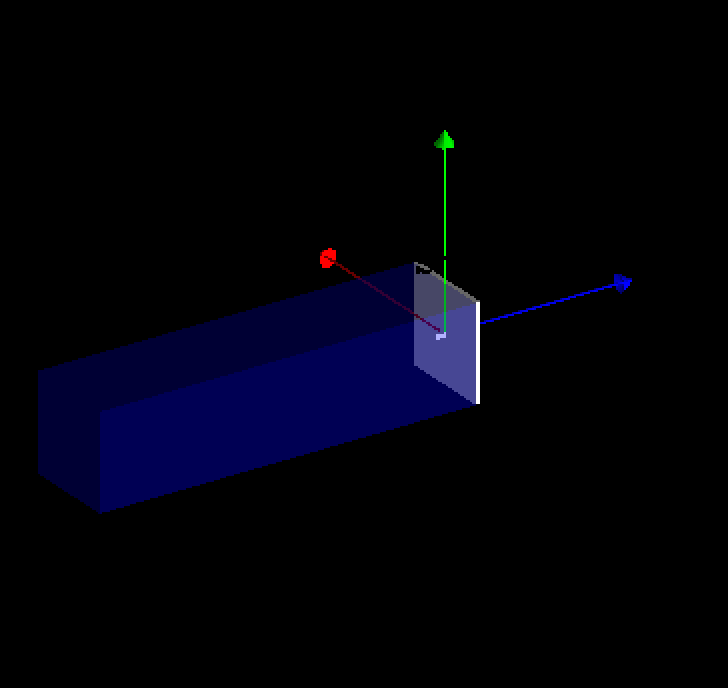
\includegraphics[width=0.6\columnwidth]{detector2.png}
  \caption{Configuration used in the second part of the experiment. The arrows represent the x (red), y (green) and z (blue) axis. The image was realized with Geant4.}
  \label{fig:conf2}
\end{figure}
For the second part we used the configuration shown in Fig.~\ref{fig:conf2}. It consists of the same detector used before (with a fixed thickness of 5 mm) and of an aluminum box shaped located inside a box of water. The box of water is 10 cm x 10 cm x 40 cm while the aluminium box has a frontal area of 0.5 cm x 0.5 cm and a thickness of 4 mm, 6 mm, 8 mm and 10 mm, for an amount of four conditions. The source is positioned at a distance of 20 cm from the detector and is made of $4*10^{6}$ photons of energy equal to 40 keV; it emits with an opening angle of 8 degrees.

The aim of this second part is to use the histograms of photons detected to calculate the contrast between the aluminium box and the background (detector). Calling $I_{b}$ the average intensity of the background and $I_{a}$ the average intensity of the part behind the aluminum box, we have compute the contrast $C$ using the following:
\begin{equation}
  C=\frac{I_{b}-I_{a}}{I_{b}}
  \label{eq:contrast}
\end{equation}

\subsection{Results and discussion}
\begin{table}[H]
  \centering
  \begin{tabular}{|c|c|c|c|}
    \hline
    Box thickness (mm) & $I_{b}$ & $I_{a}$ & $C$ \\
    \hline
    4 & & & \\
    \hline
    6 & & & \\
    \hline
    8 & & & \\
    \hline
    10 & & & \\
    \hline
  \end{tabular}
  \caption{Results of part two.}
  \label{tab:part_two}
\end{table}

\clearpage


\appendix

\section{Plots for the first part}
\label{sec:appendix_1}

\begin{figure}[H]
  \centering
  \subfloat[][$\gamma$ energy $=$ 10 KeV] {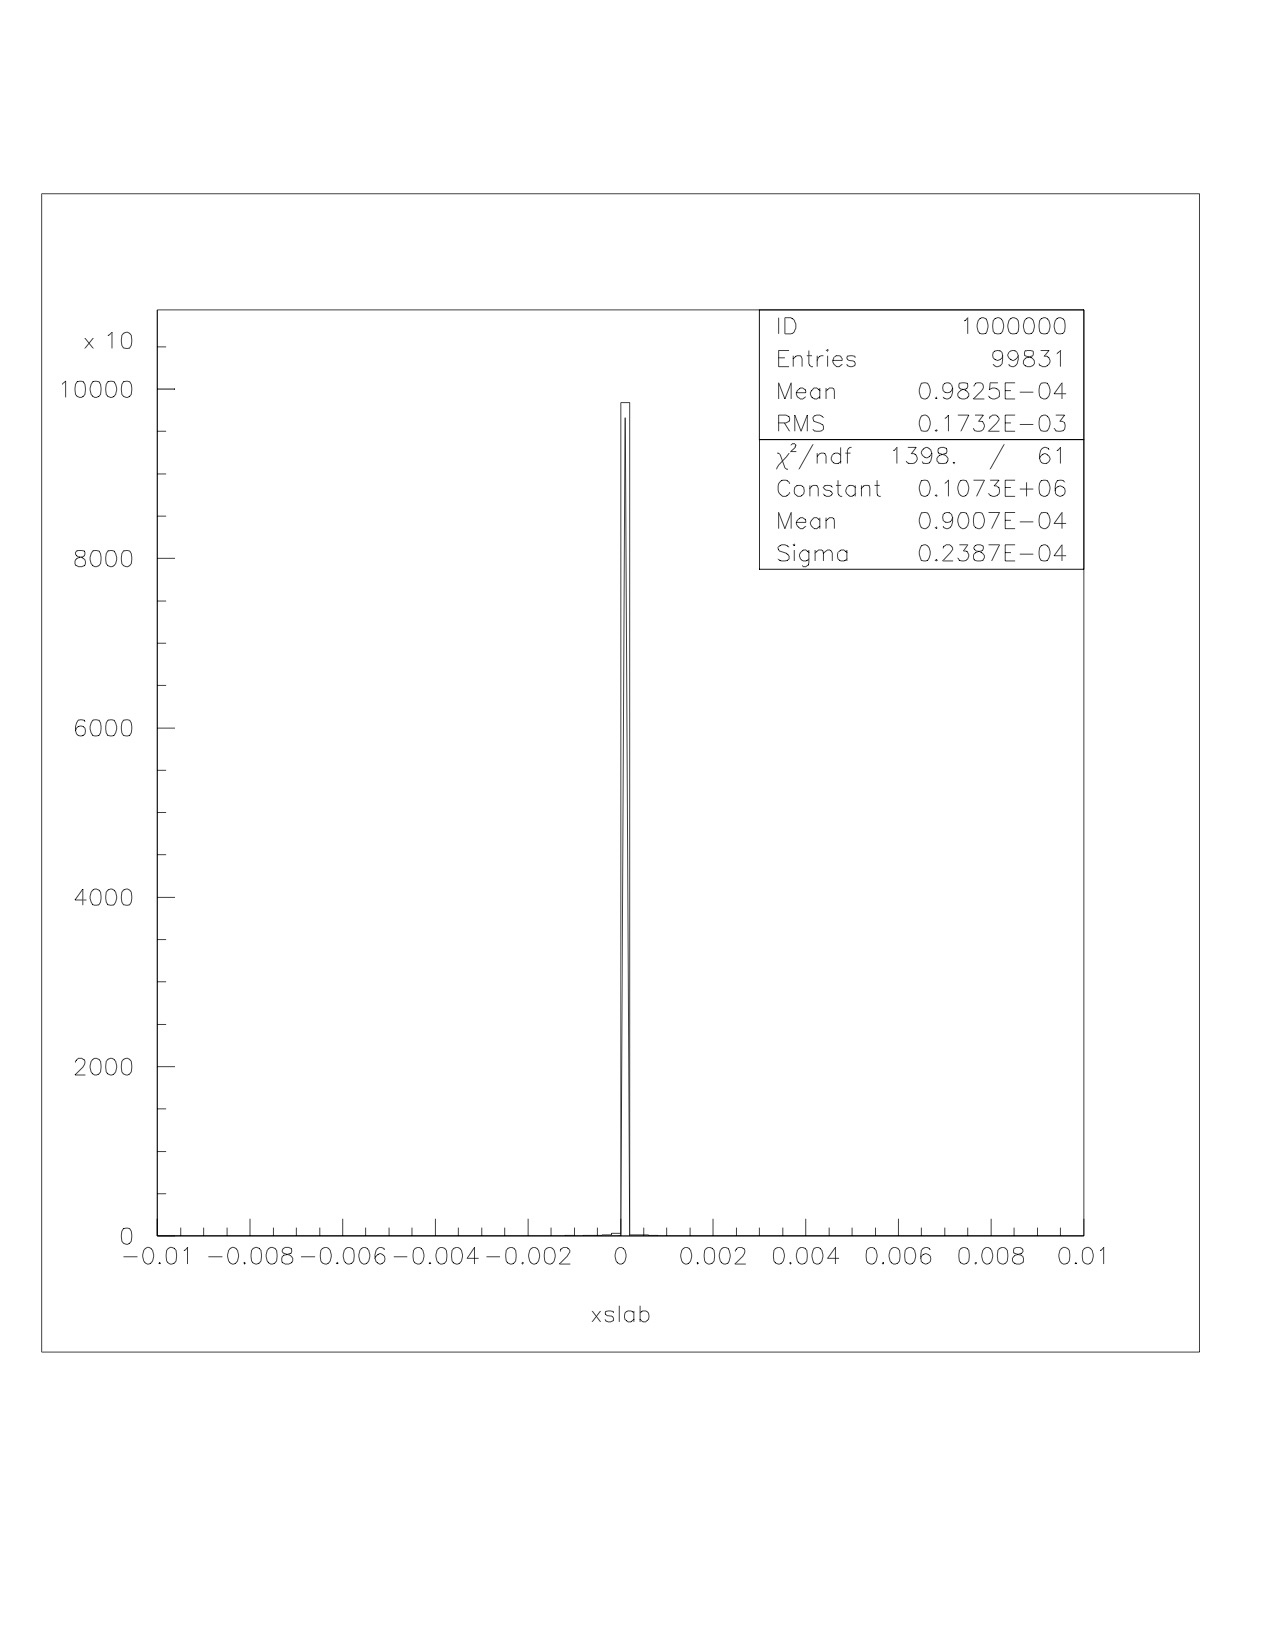
\includegraphics[width=0.45\textwidth]{ex_images/1_005_010_xslab.jpg}}
  \subfloat[][$\gamma$ energy $=$ 30 KeV] {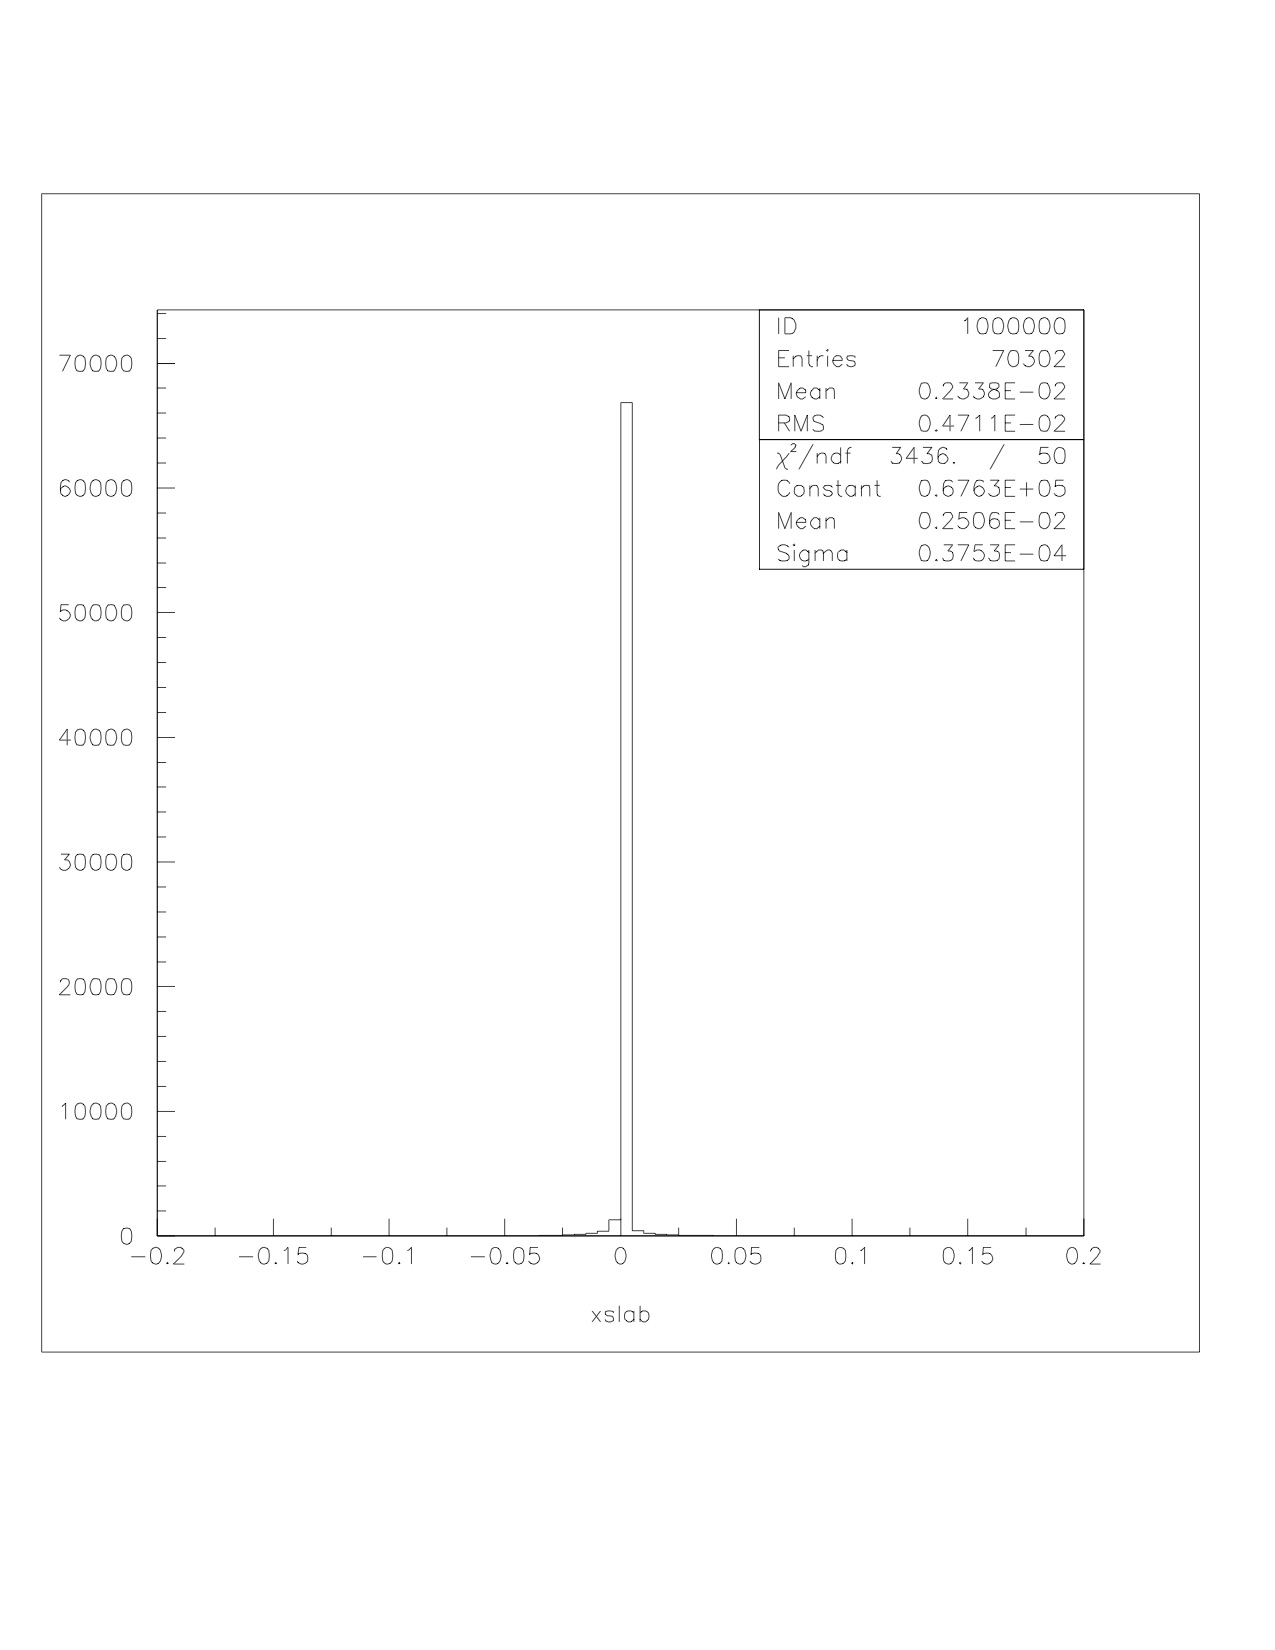
\includegraphics[width=0.45\textwidth]{ex_images/1_005_030_xslab.jpg}}\\
  \subfloat[][$\gamma$ energy $=$ 50 KeV] {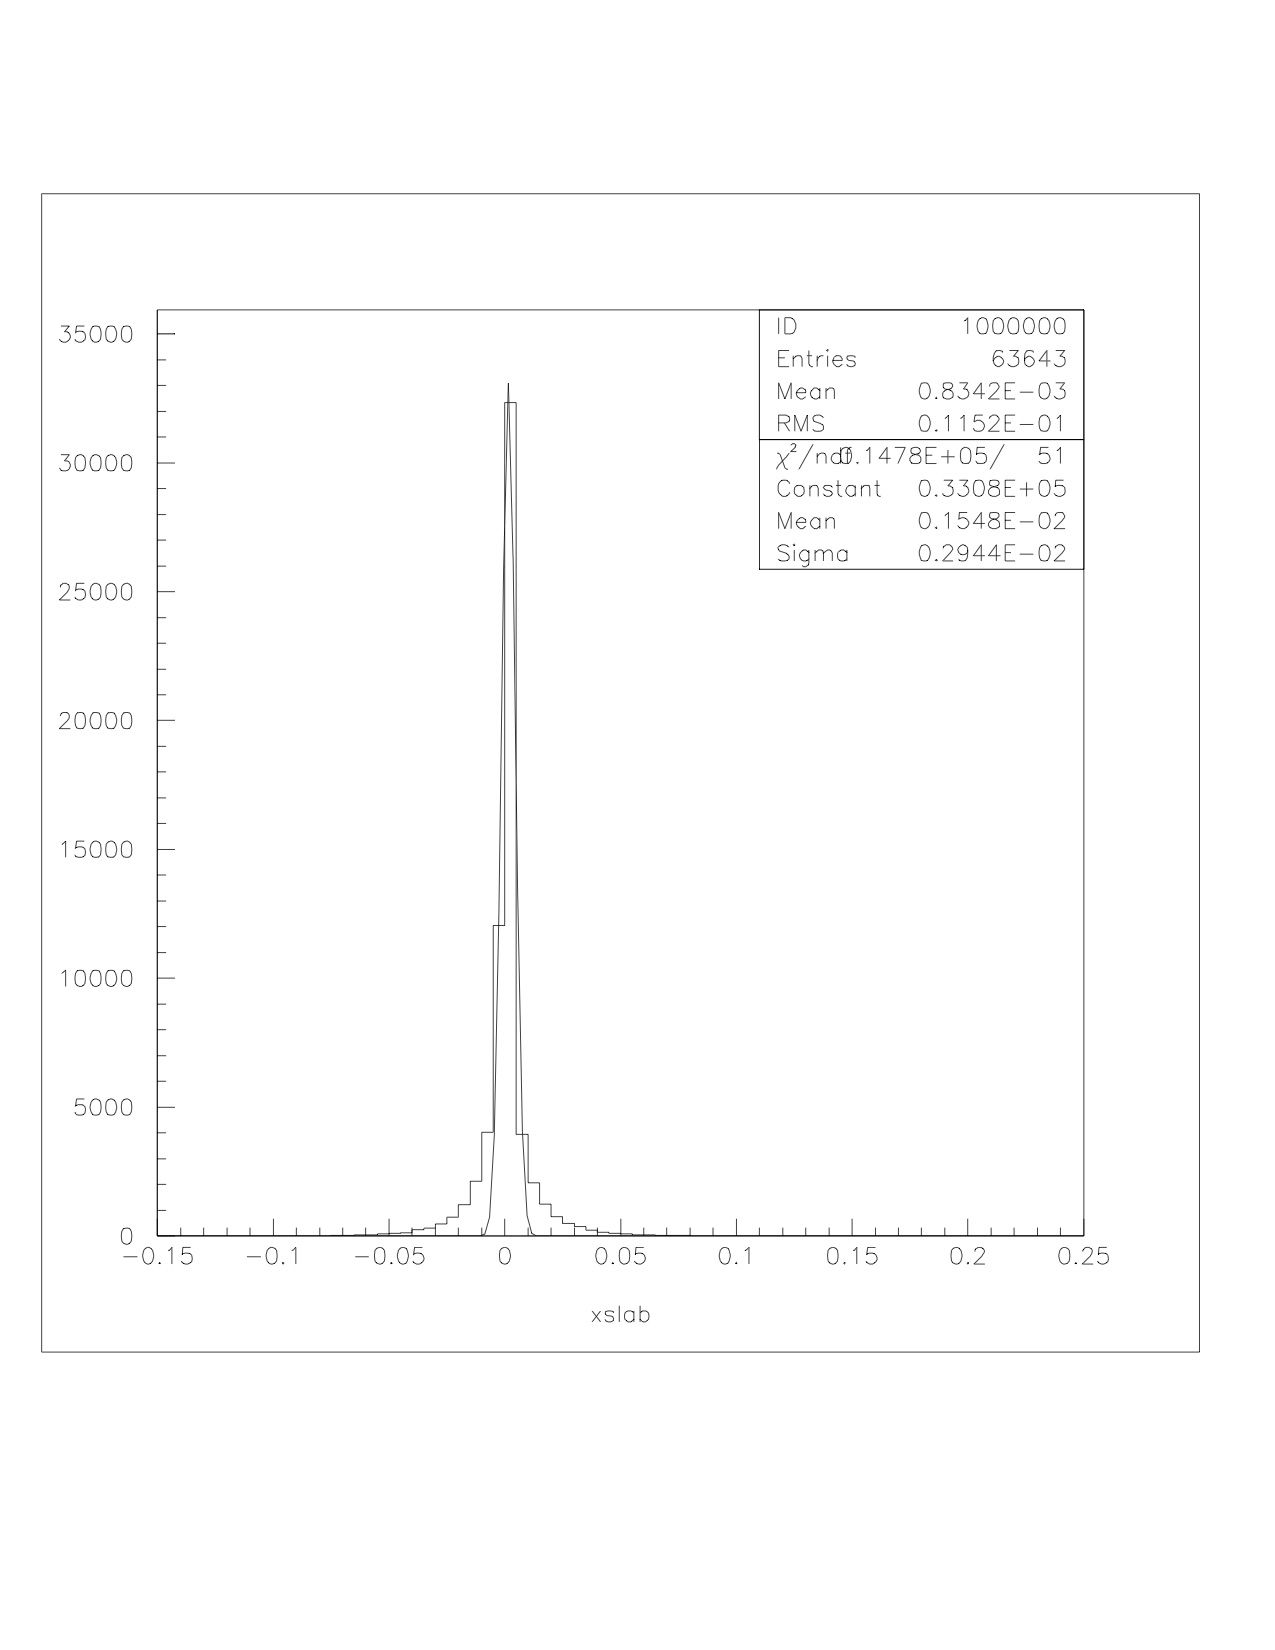
\includegraphics[width=0.45\textwidth]{ex_images/1_005_050_xs.jpg}}
  \subfloat[][$\gamma$ energy $=$ 140 KeV] {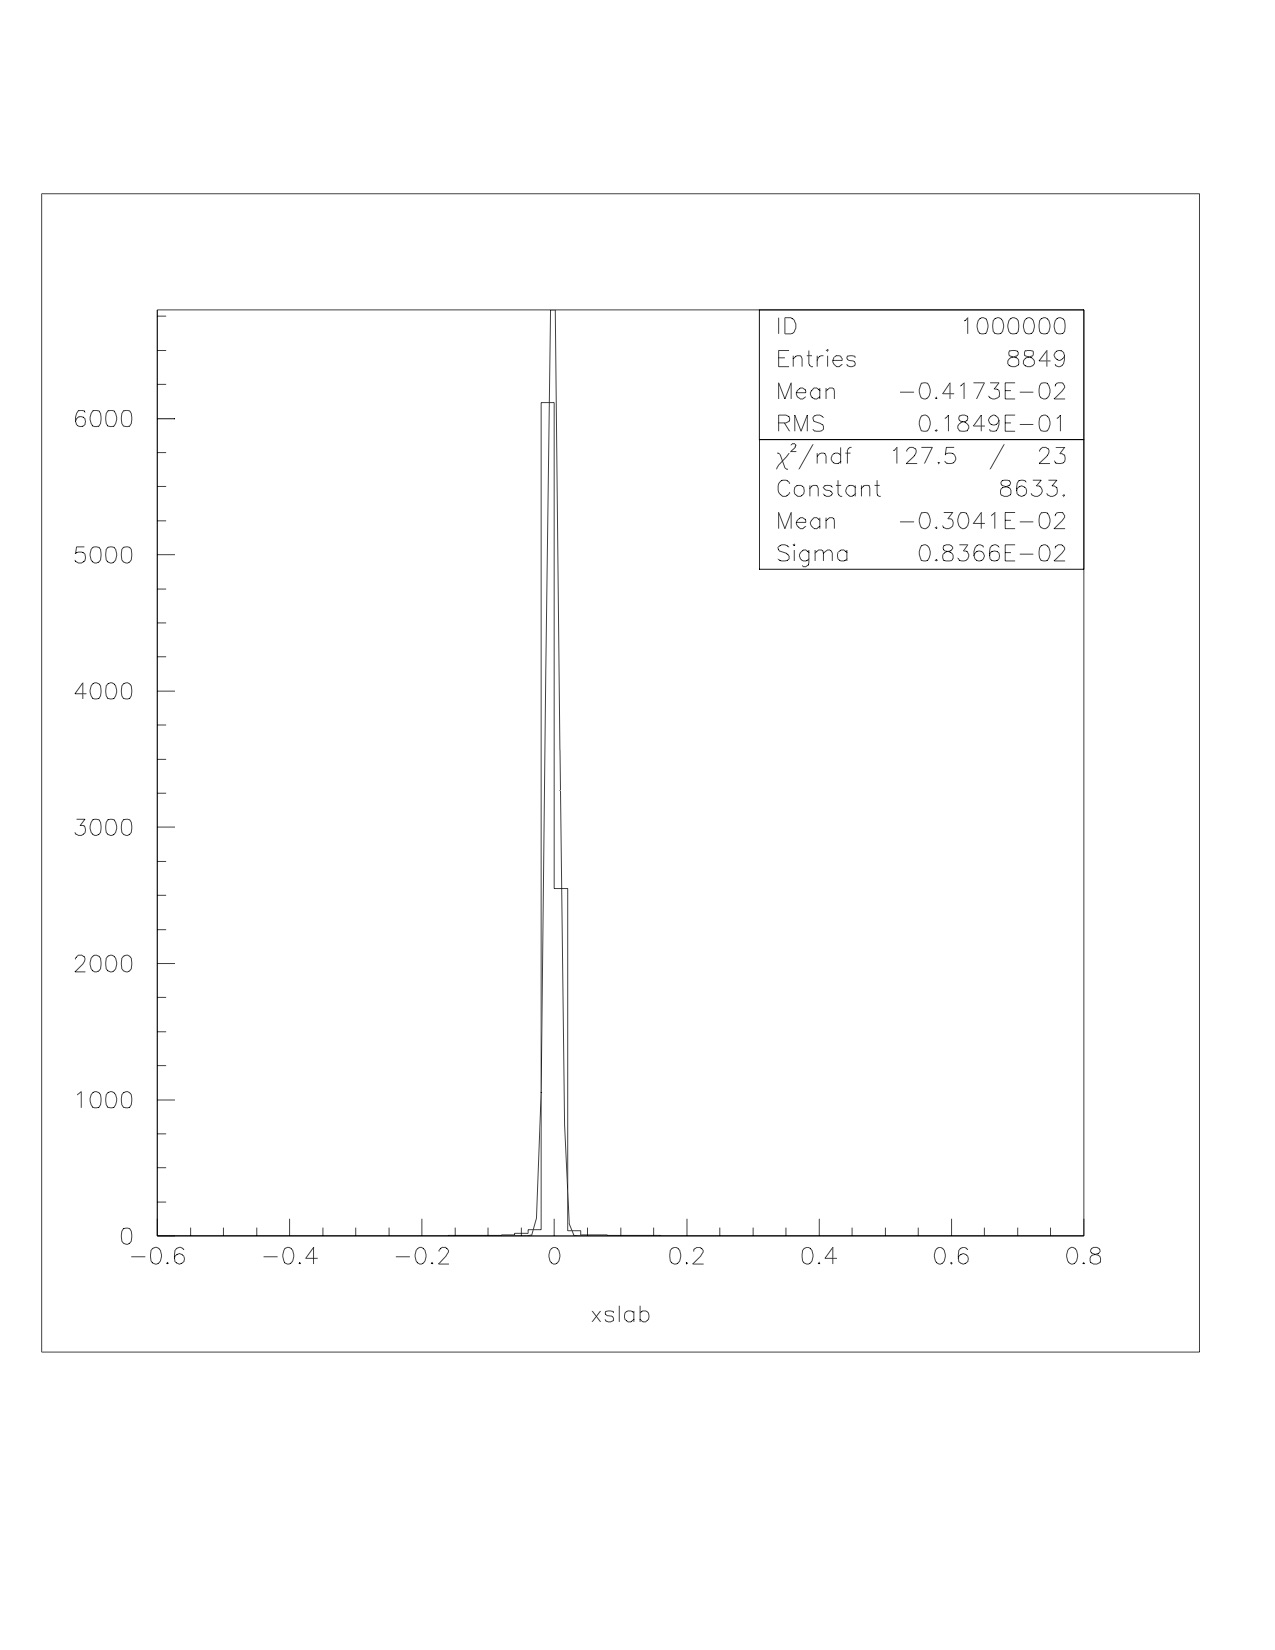
\includegraphics[width=0.45\textwidth]{ex_images/1_005_140_xs.jpg}}
  \caption{PSF plots with detector thickness of 0.5 mm, no blur.}
  \label{fig:005_xs}
\end{figure}

\begin{figure}[H]
  \centering
  \subfloat[][$\gamma$ energy $=$ 10 KeV] {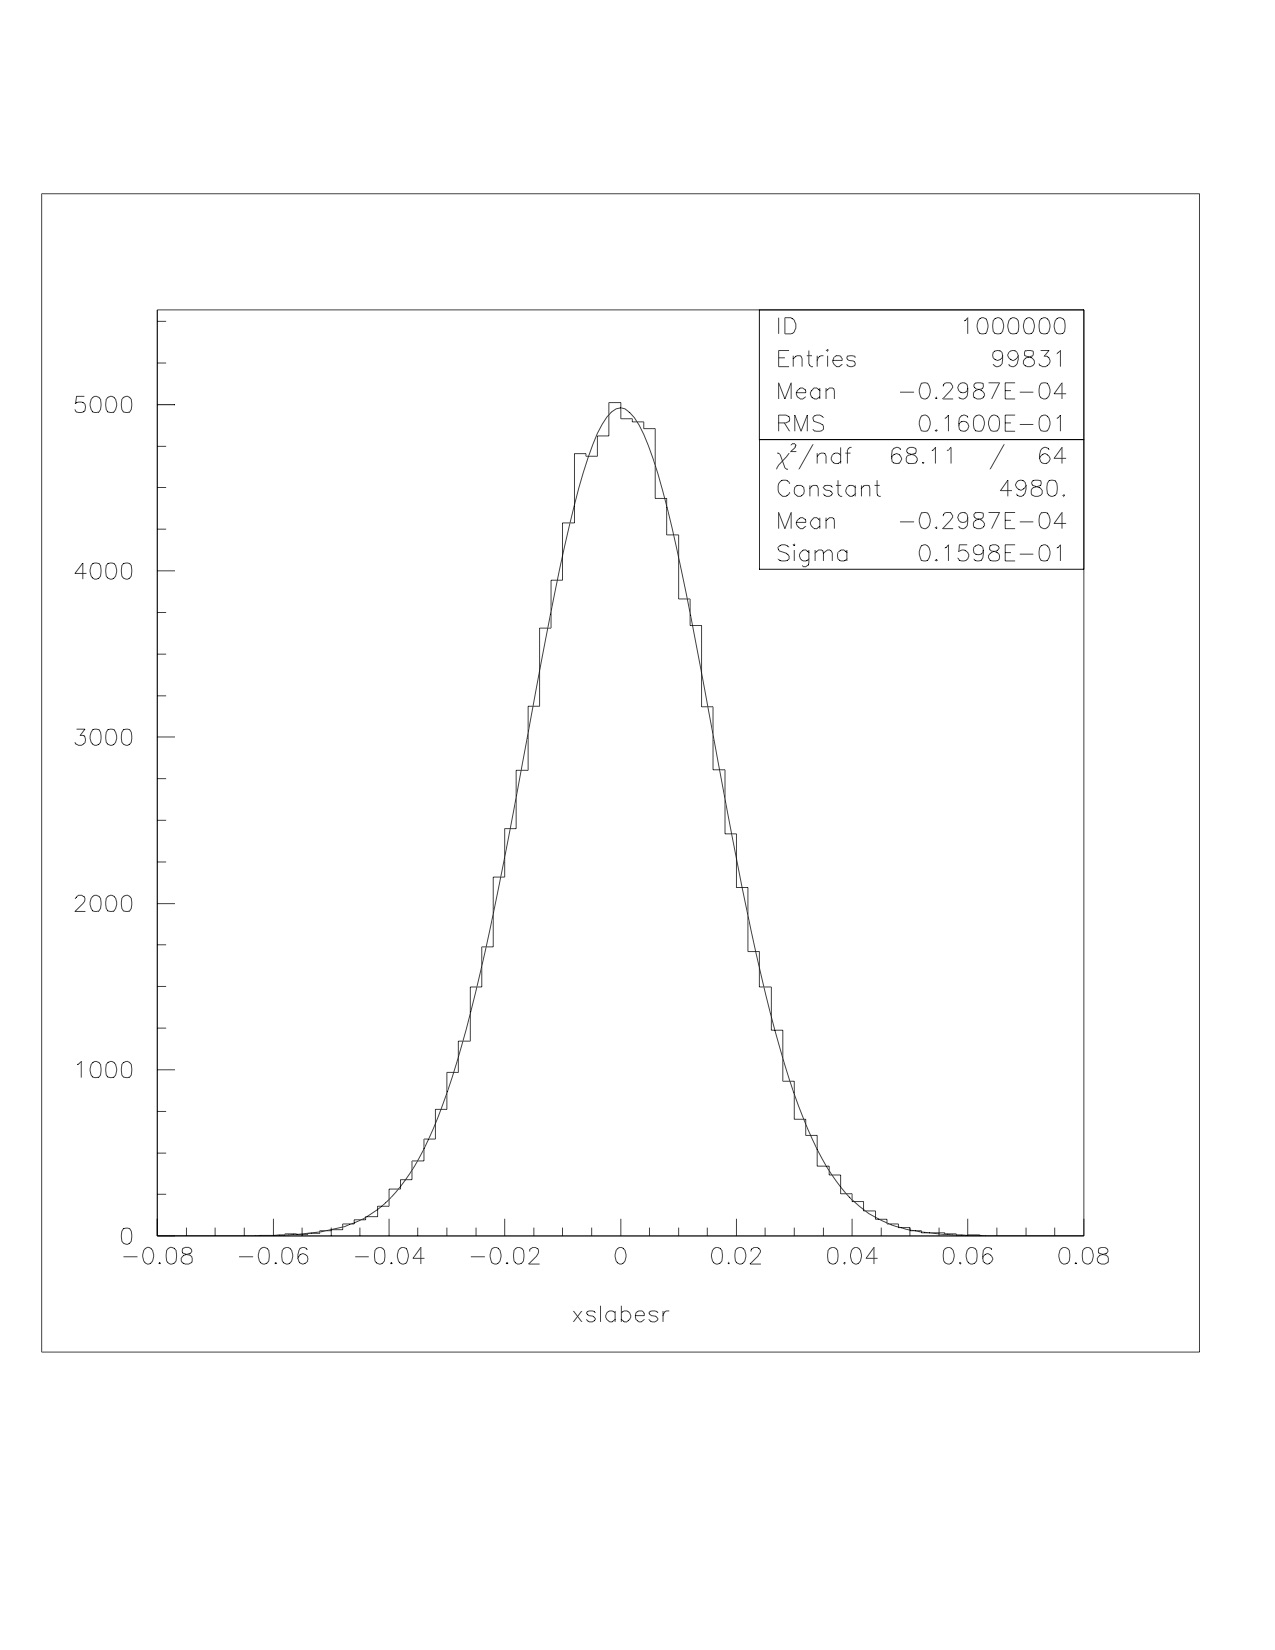
\includegraphics[width=0.45\textwidth]{ex_images/1_005_010_xslabesr.jpg}}
  \subfloat[][$\gamma$ energy $=$ 30 KeV] {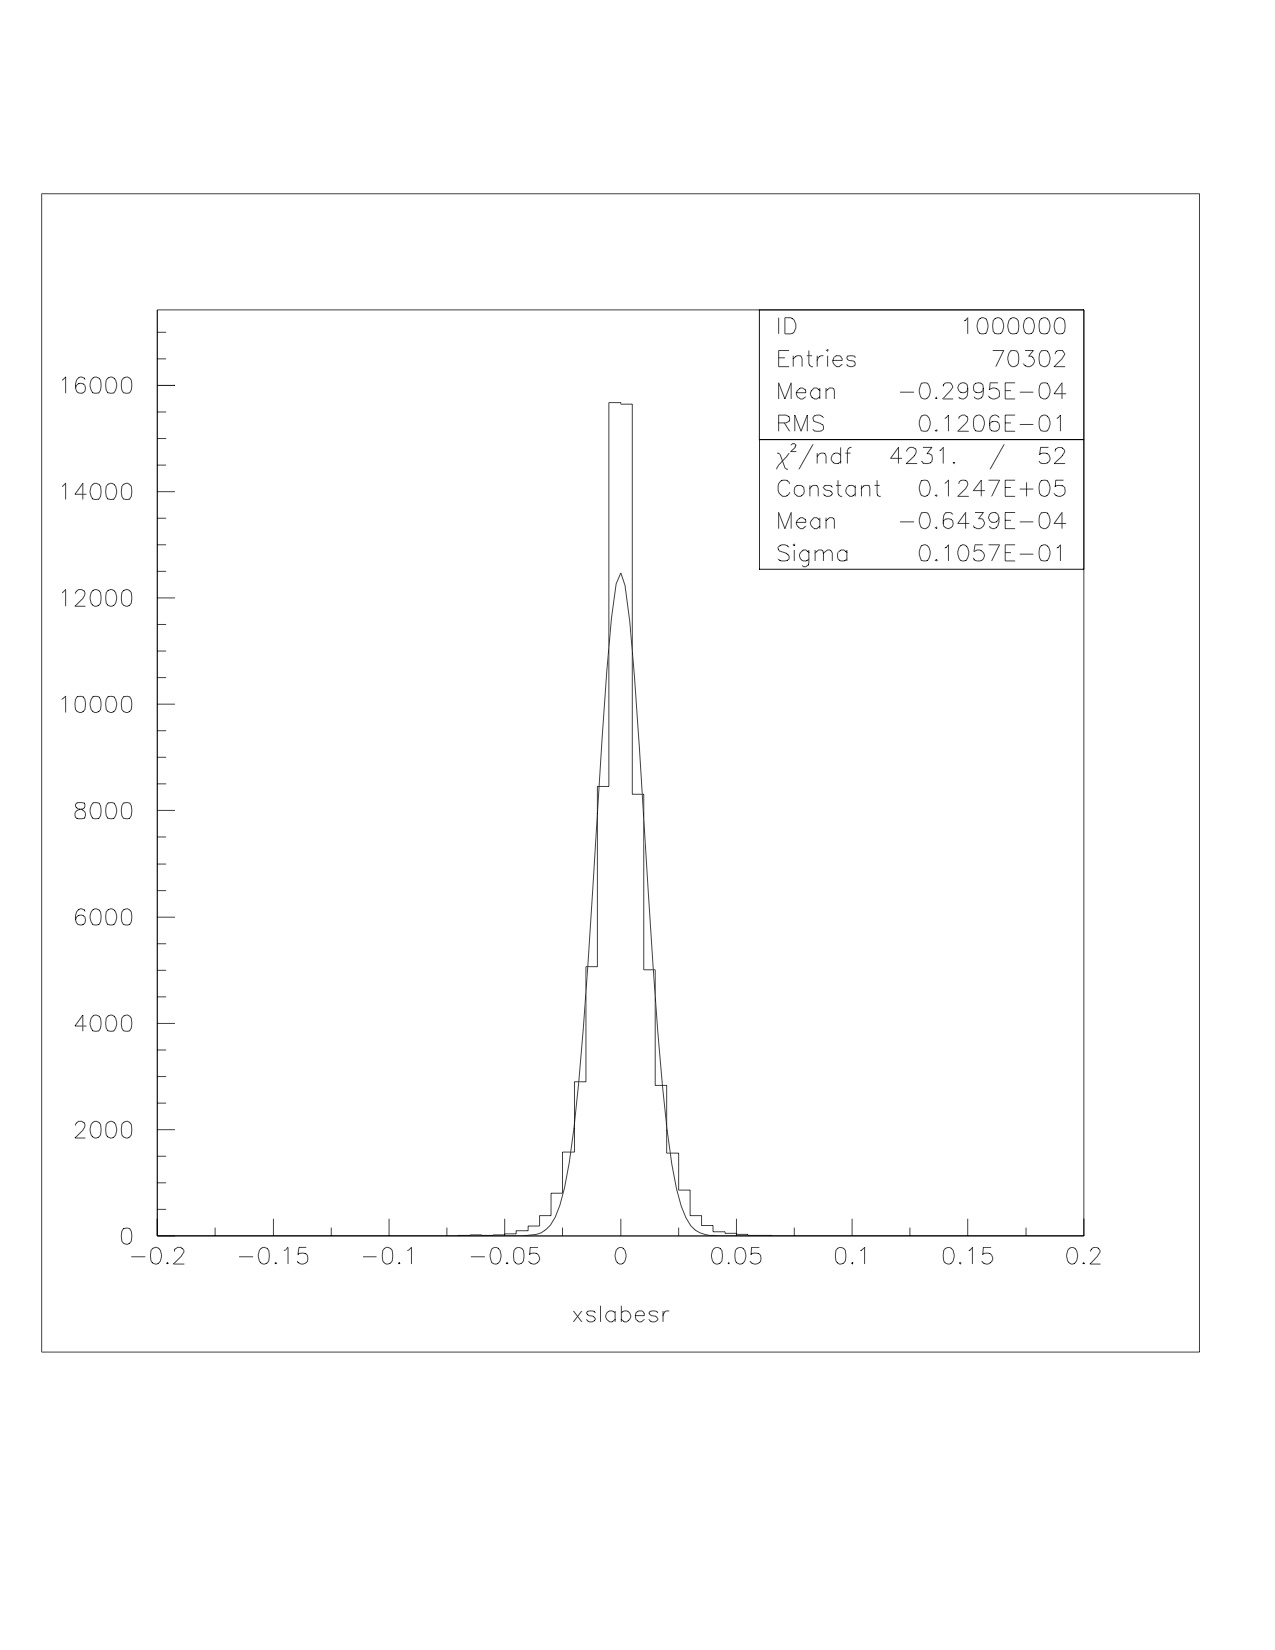
\includegraphics[width=0.45\textwidth]{ex_images/1_005_030_xse.jpg}}\\
  \subfloat[][$\gamma$ energy $=$ 50 KeV] {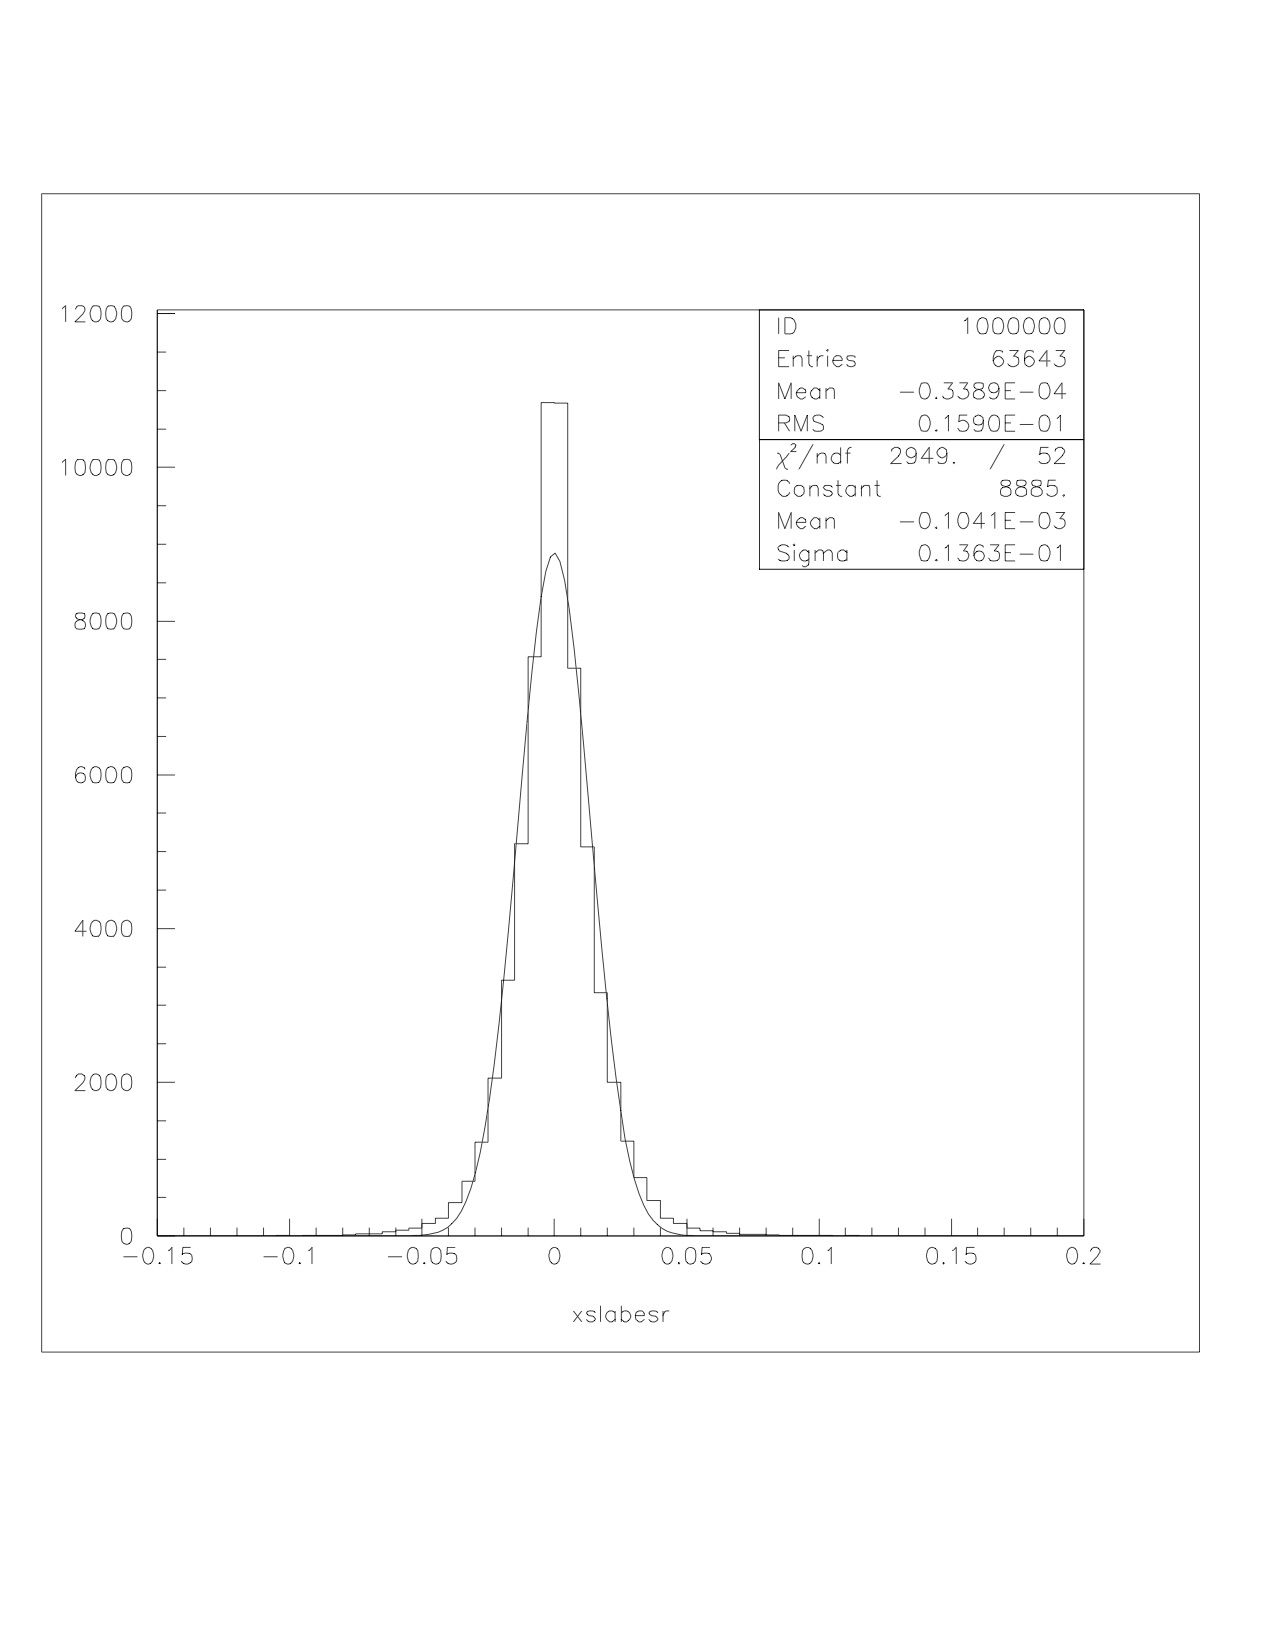
\includegraphics[width=0.45\textwidth]{ex_images/1_005_050_xse.jpg}}
  \subfloat[][$\gamma$ energy $=$ 140 KeV] {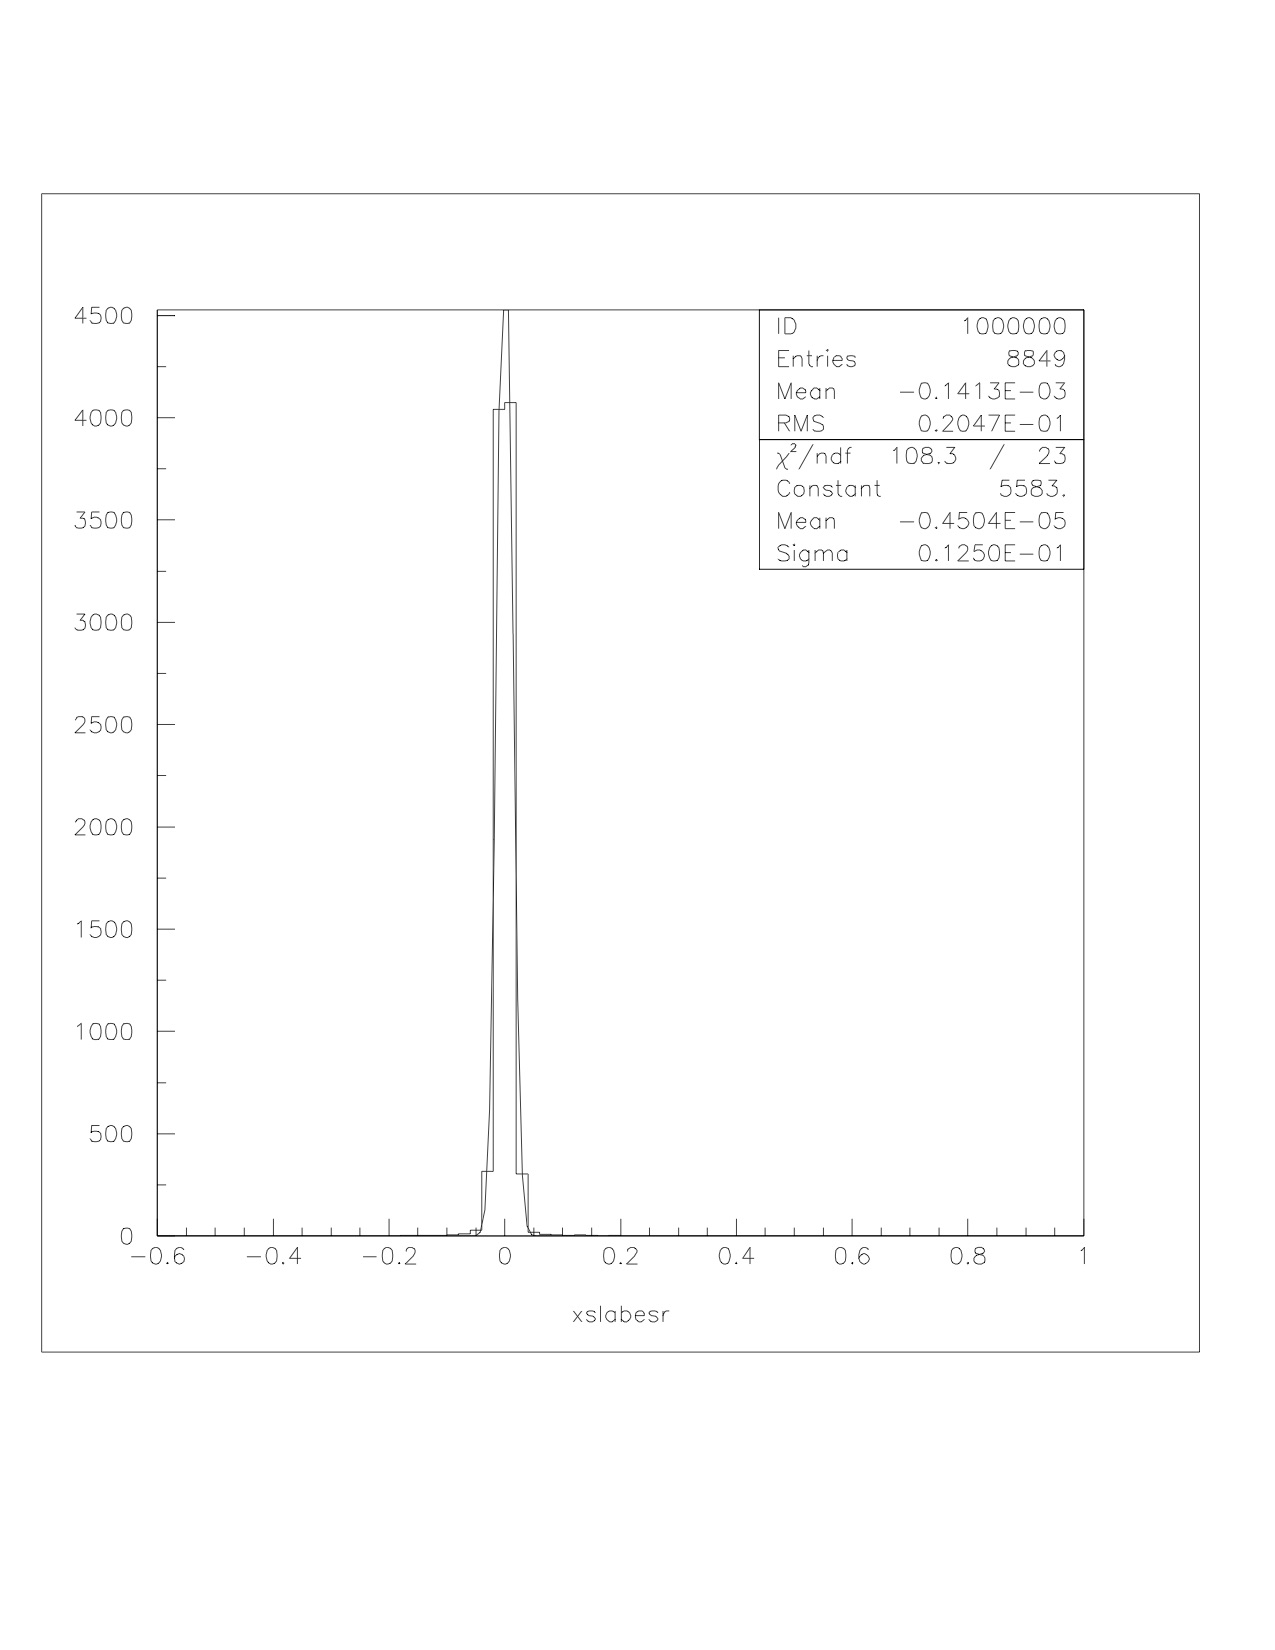
\includegraphics[width=0.45\textwidth]{ex_images/1_005_140_xse.jpg}}
  \caption{PSF plots with detector thickness of 0.5 mm, with blur.}
  \label{fig:005_xse}
\end{figure}

\begin{figure}[H]
  \centering
  \subfloat[][$\gamma$ energy $=$ 10 KeV] {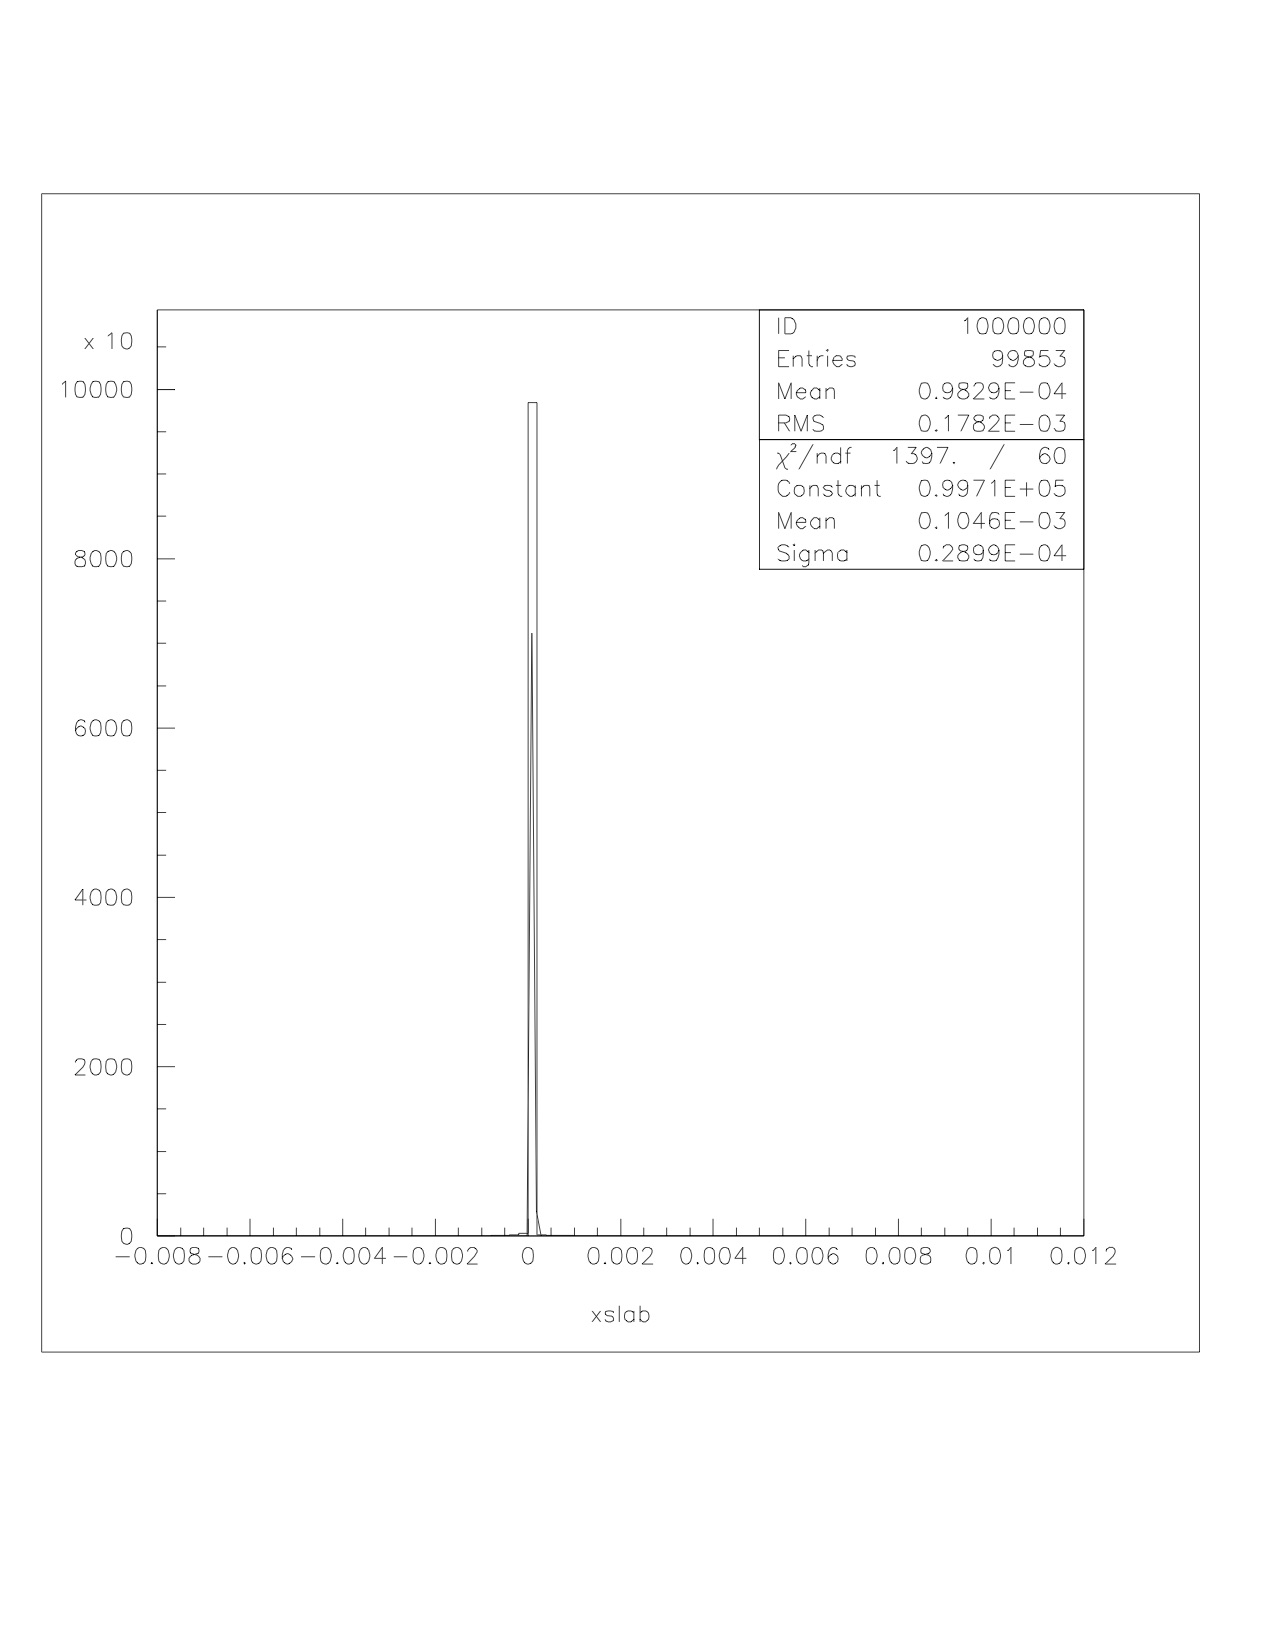
\includegraphics[width=0.45\textwidth]{ex_images/1_010_010_xs.jpg}}
  \subfloat[][$\gamma$ energy $=$ 10 KeV] {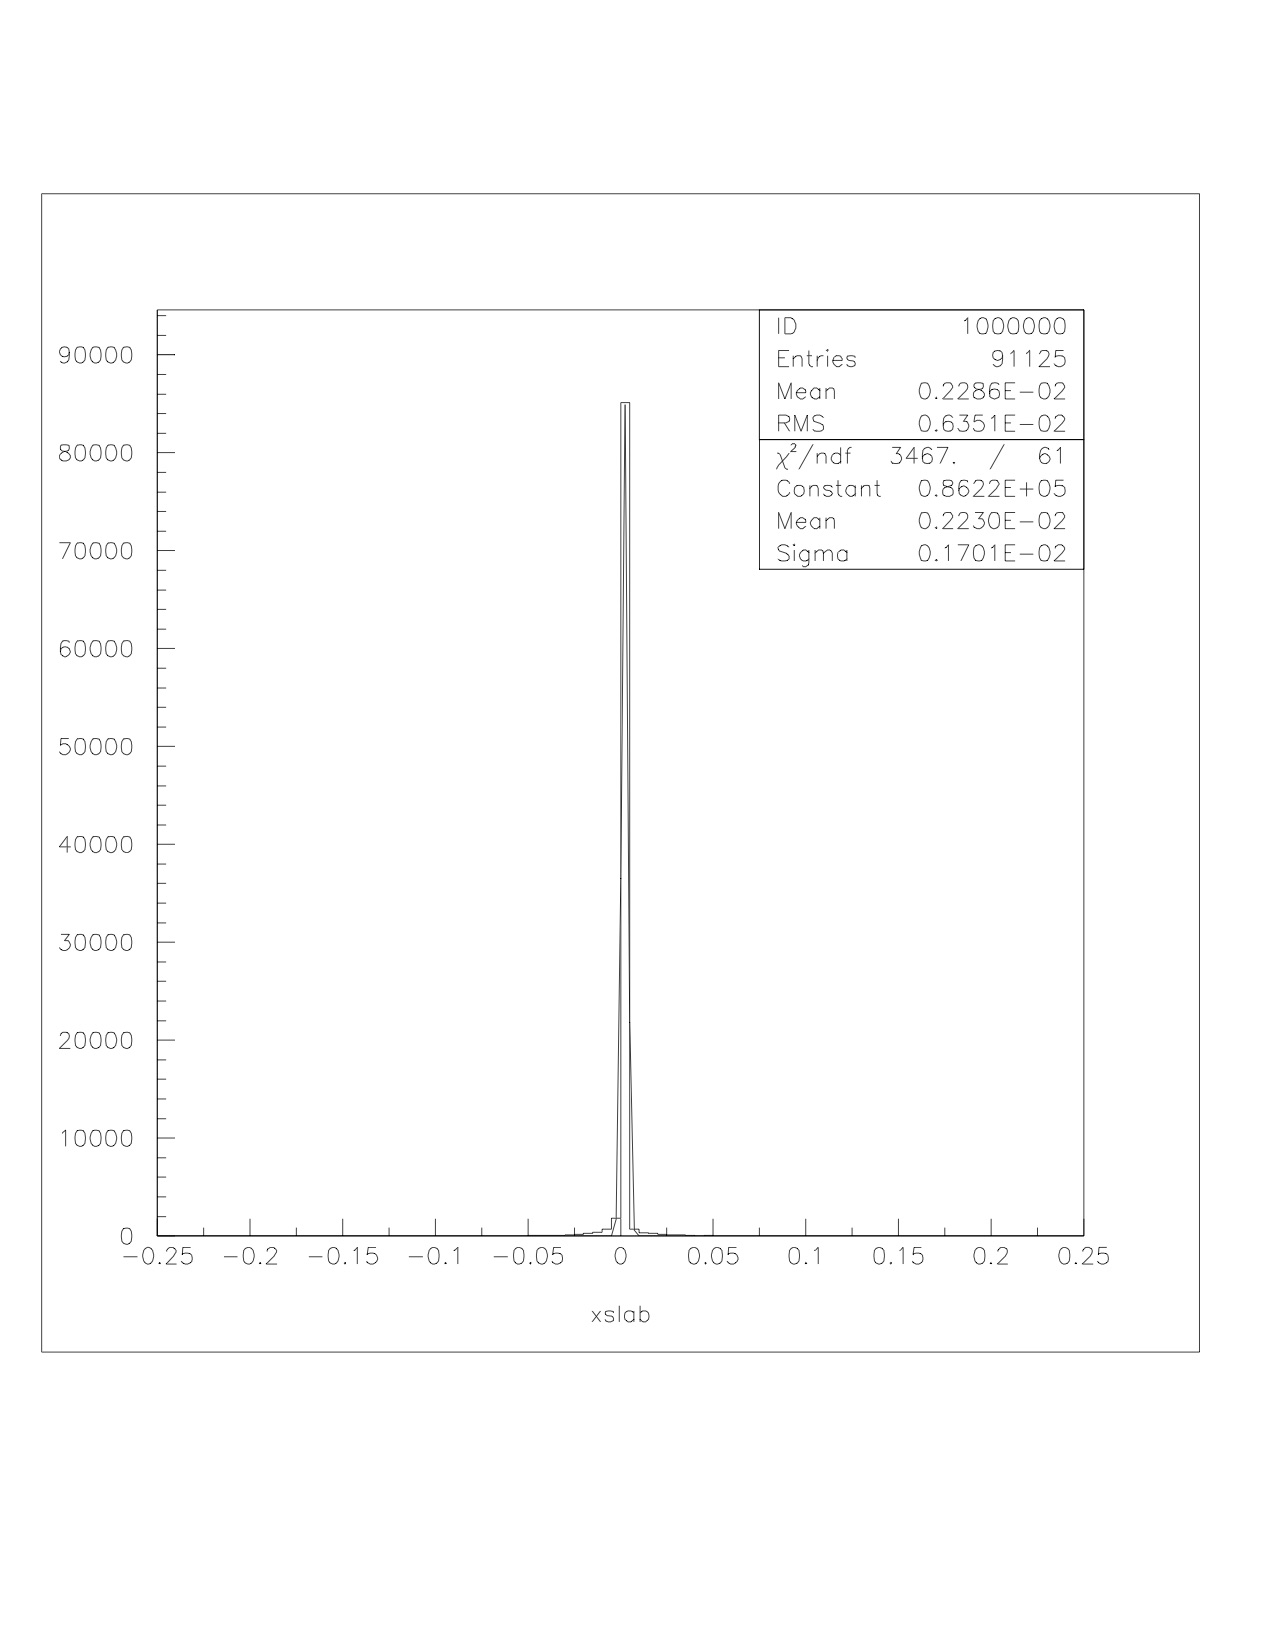
\includegraphics[width=0.45\textwidth]{ex_images/1_010_030_xs.jpg}}\\
  \subfloat[][$\gamma$ energy $=$ 10 KeV] {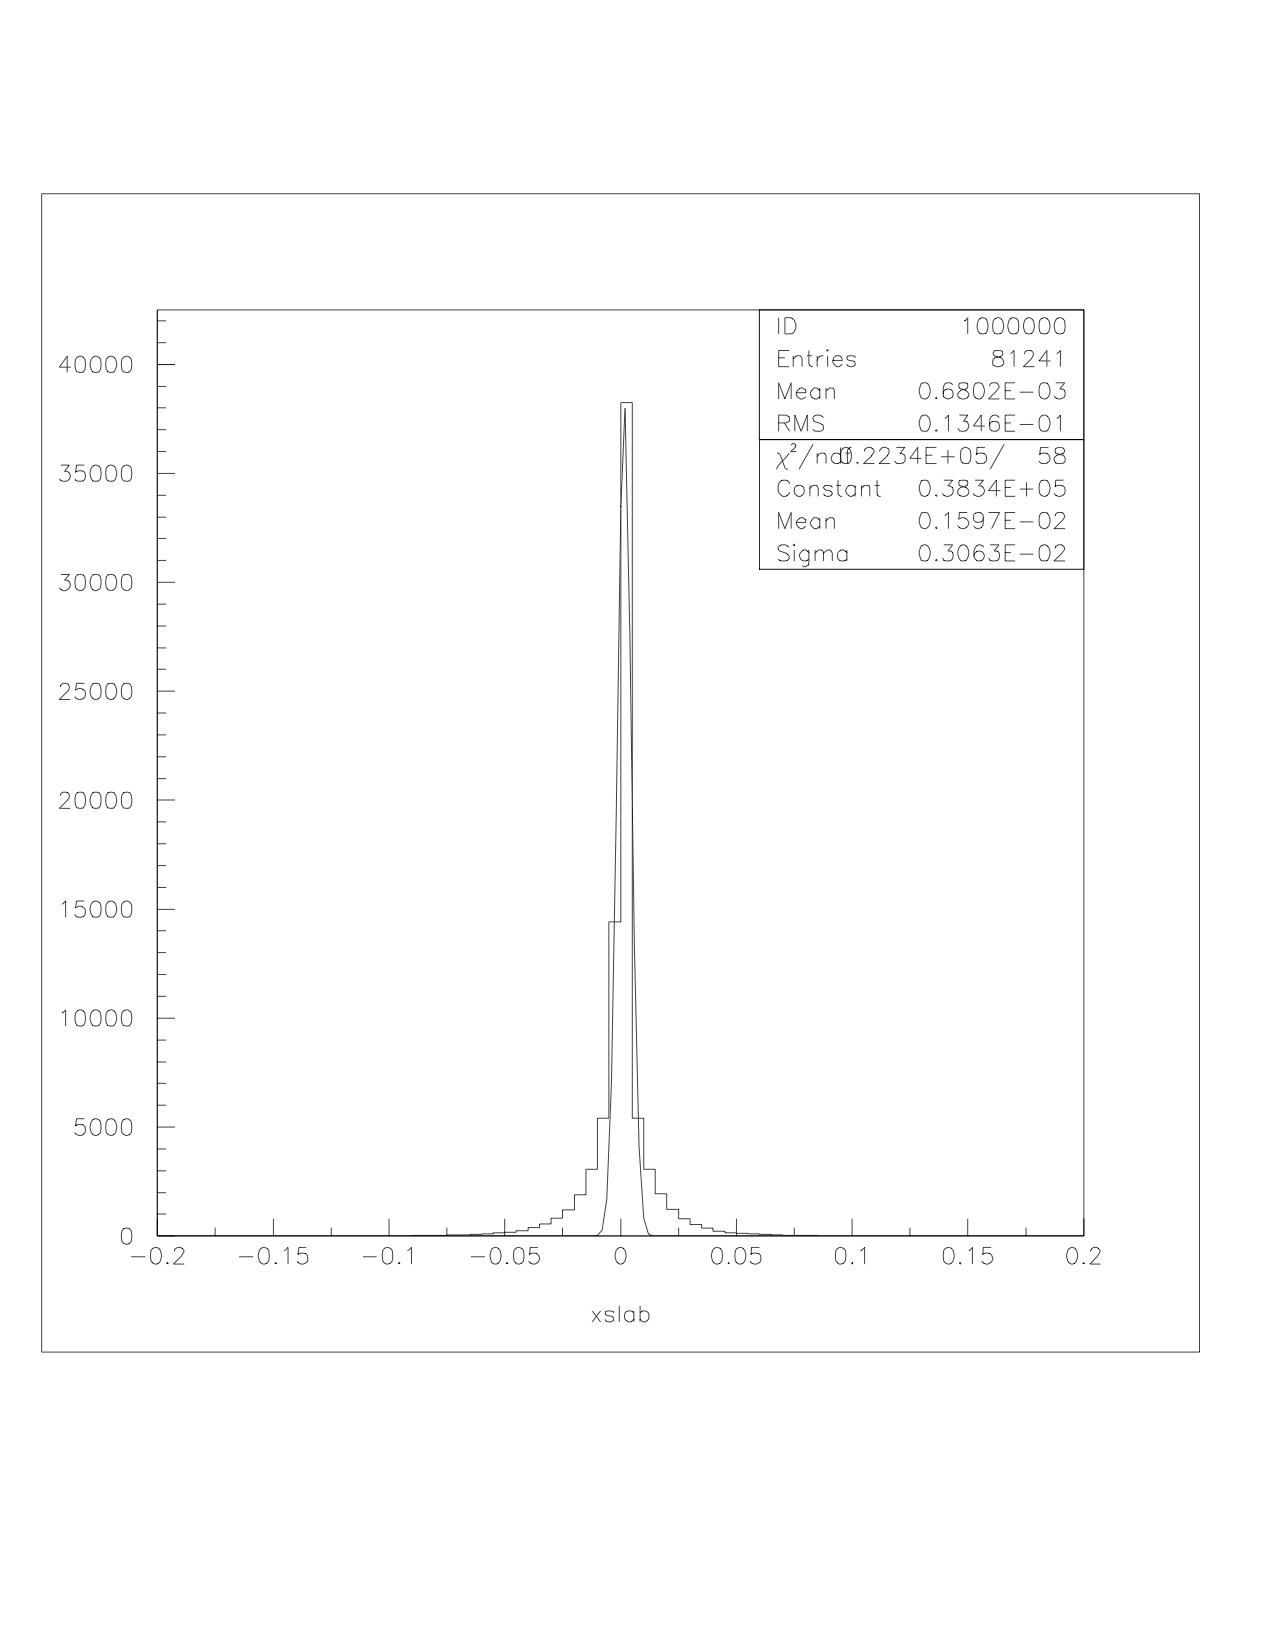
\includegraphics[width=0.45\textwidth]{ex_images/1_010_050_xs.jpg}}
  \subfloat[][$\gamma$ energy $=$ 10 KeV] {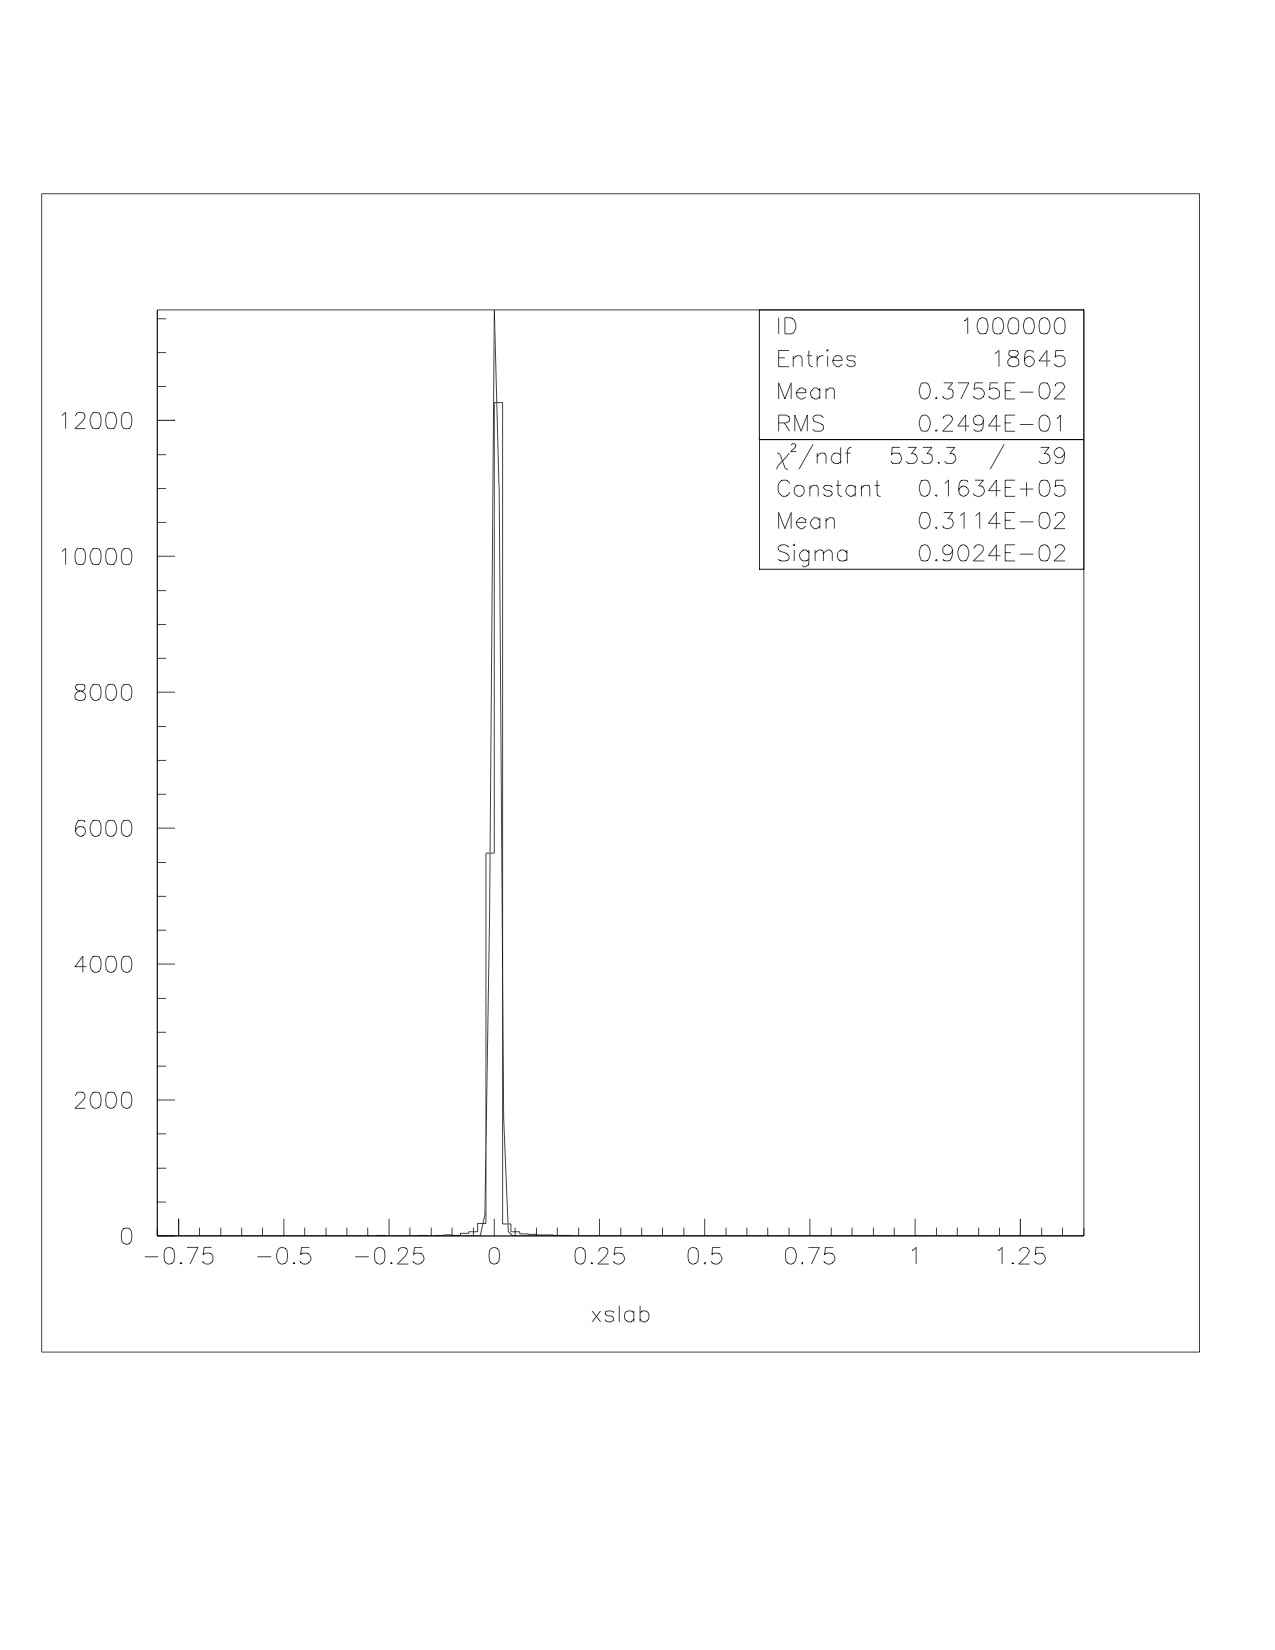
\includegraphics[width=0.45\textwidth]{ex_images/1_010_140_xs.jpg}}
  \caption{PSF plots with detector thickness of 1 mm, no blur.}
  \label{fig:010_xs}
\end{figure}

\begin{figure}[H]
  \centering
  \subfloat[][$\gamma$ energy $=$ 10 KeV] {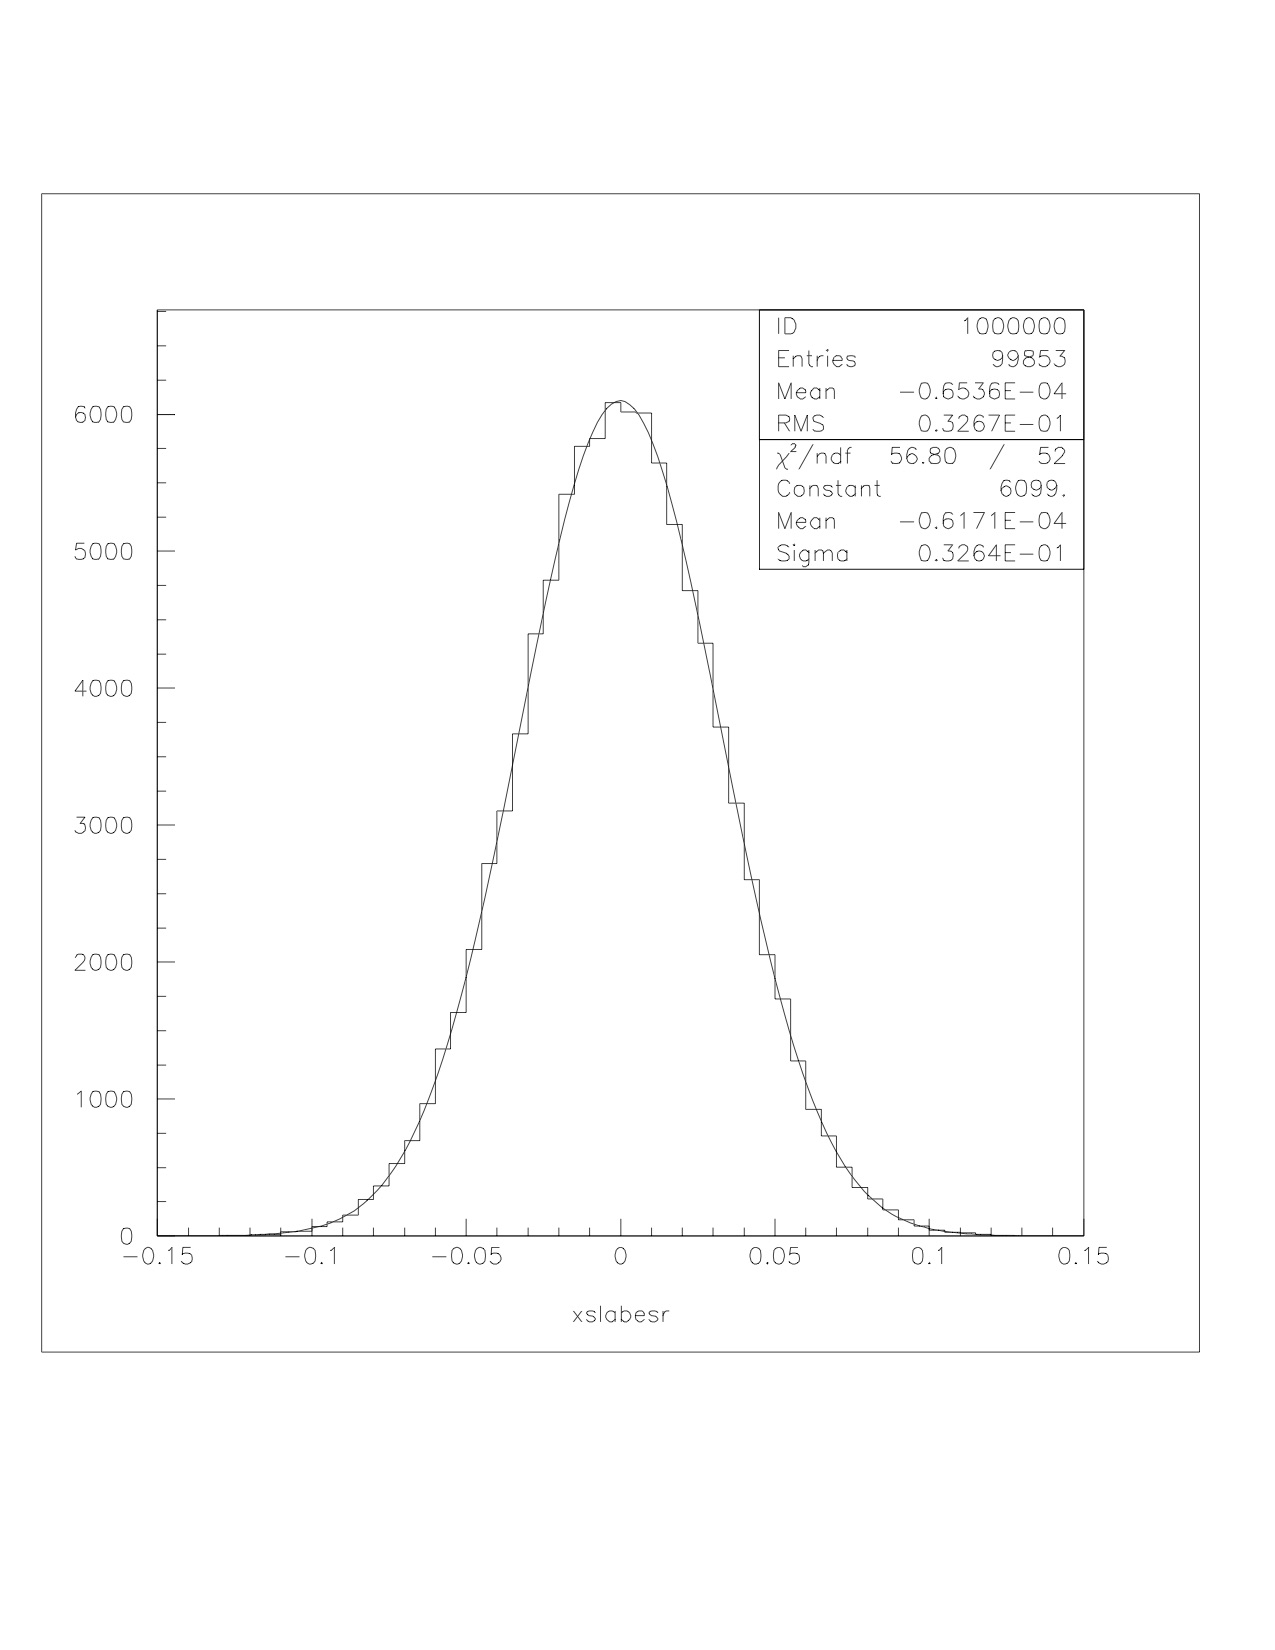
\includegraphics[width=0.45\textwidth]{ex_images/1_010_010_xse.jpg}}
  \subfloat[][$\gamma$ energy $=$ 30 KeV] {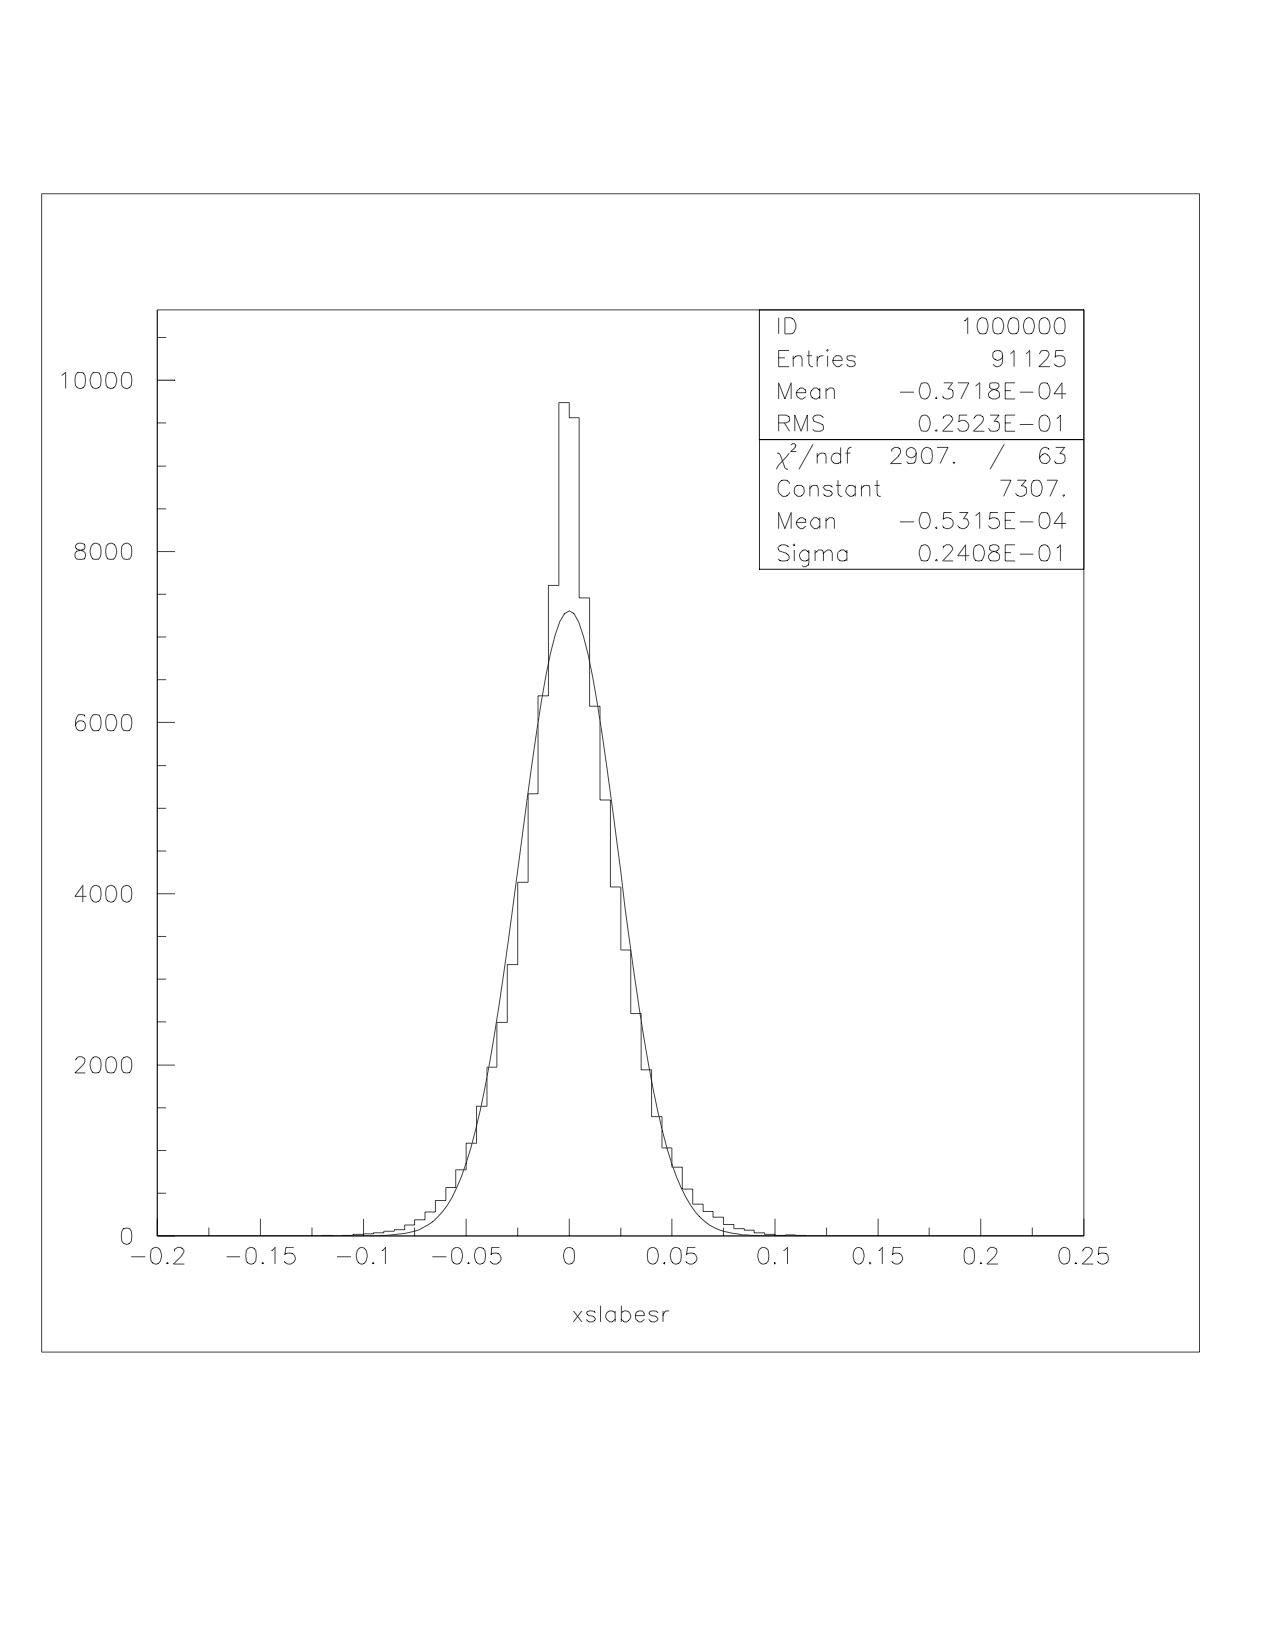
\includegraphics[width=0.45\textwidth]{ex_images/1_010_030_xse.jpg}}\\
  \subfloat[][$\gamma$ energy $=$ 50 KeV] {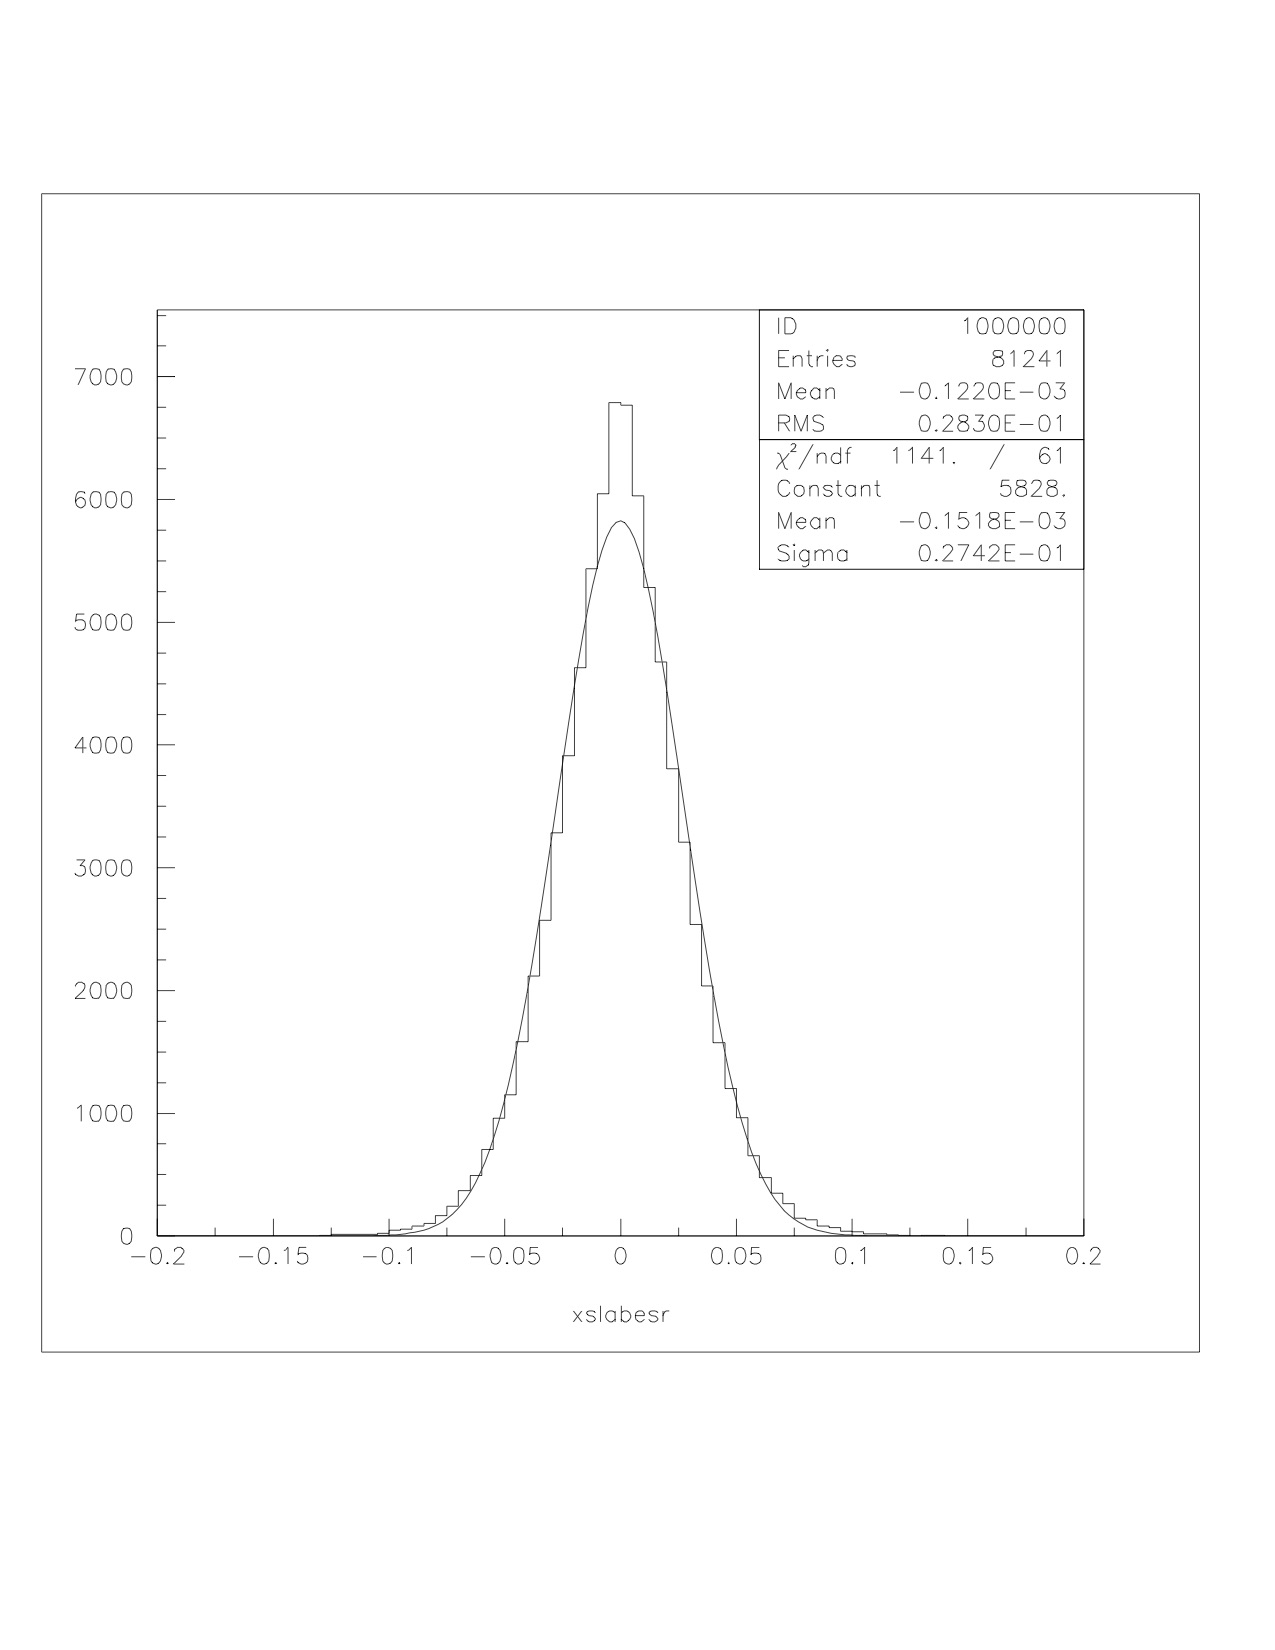
\includegraphics[width=0.45\textwidth]{ex_images/1_010_050_xse.jpg}}
  \subfloat[][$\gamma$ energy $=$ 140 KeV] {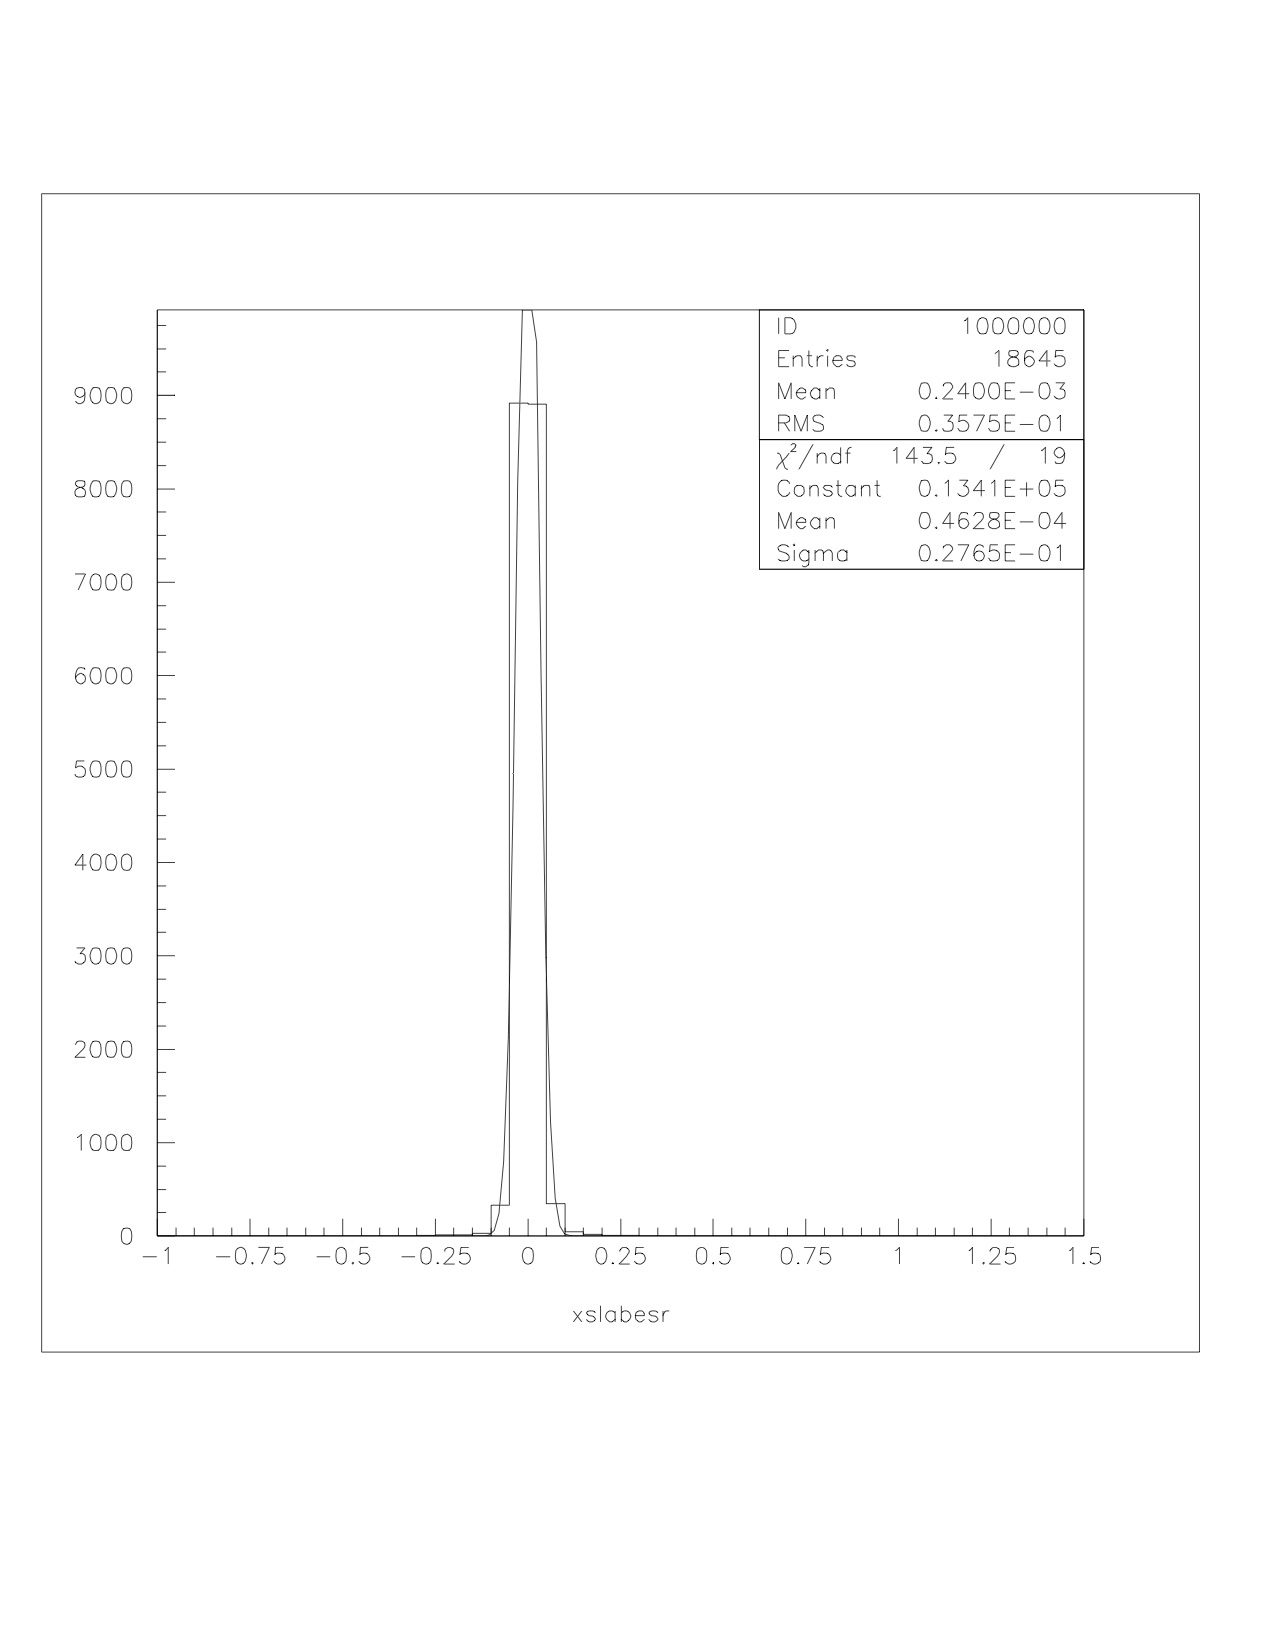
\includegraphics[width=0.45\textwidth]{ex_images/1_010_140_xse.jpg}}
  \caption{PSF plots with detector thickness of 1 mm, with blur.}
  \label{fig:010_xse}
\end{figure}

\begin{figure}[H]
  \centering
  \subfloat[][$\gamma$ energy $=$ 10 KeV] {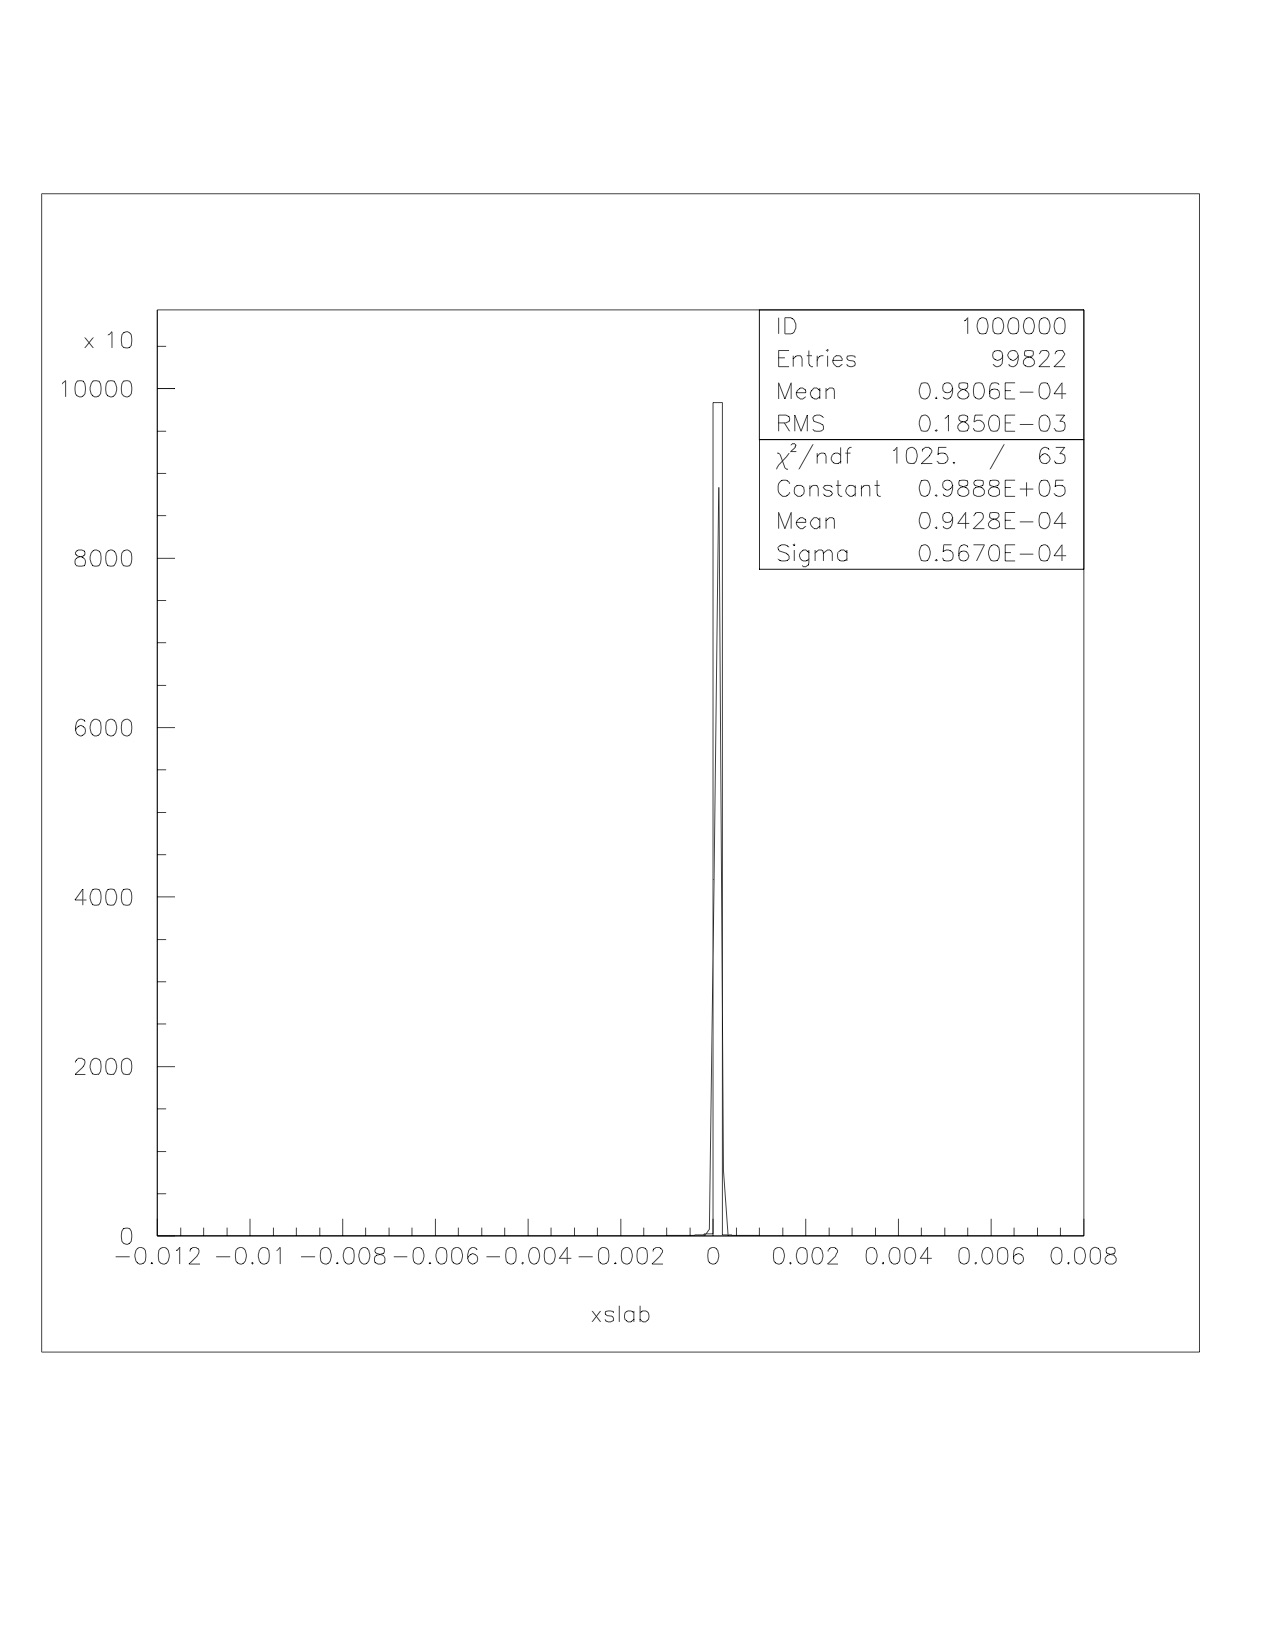
\includegraphics[width=0.45\textwidth]{ex_images/1_020_010_xs.jpg}}
  \subfloat[][$\gamma$ energy $=$ 30 KeV] {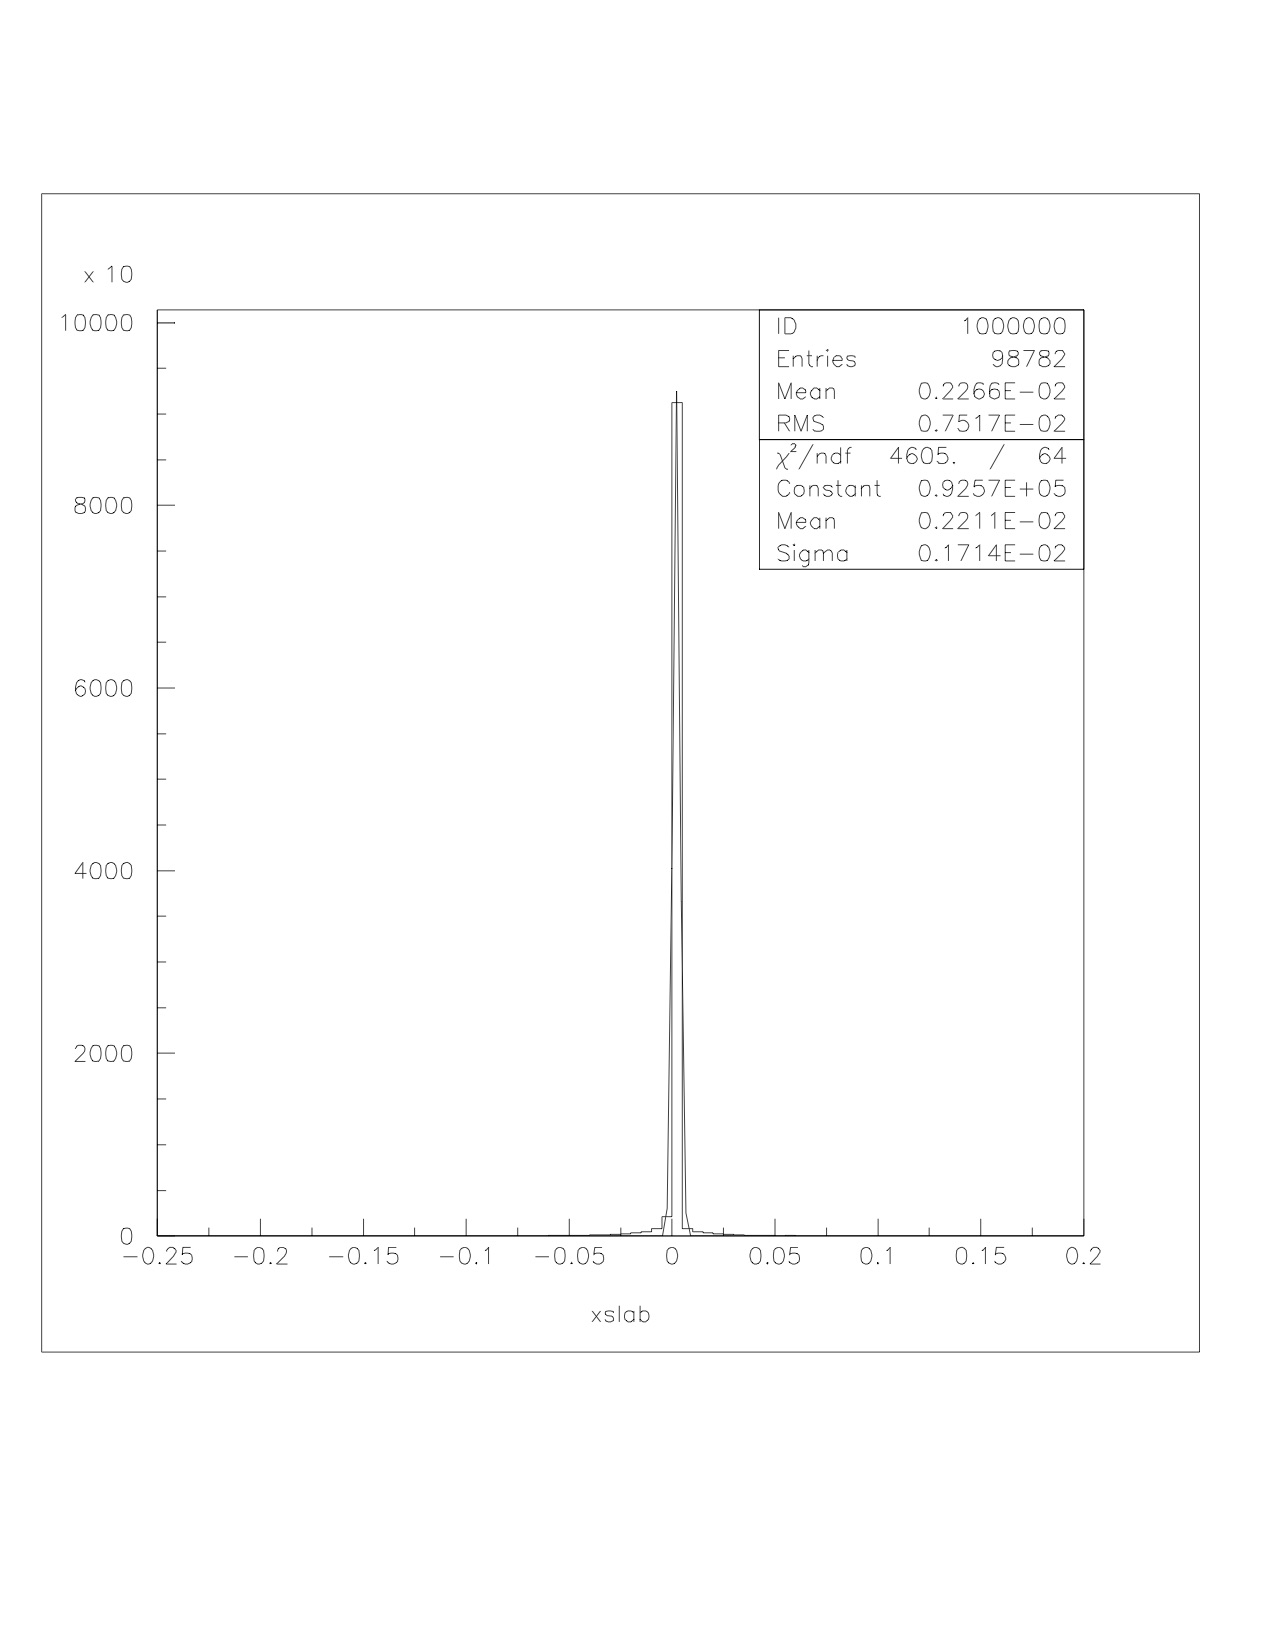
\includegraphics[width=0.45\textwidth]{ex_images/1_020_030_xs.jpg}}\\
  \subfloat[][$\gamma$ energy $=$ 50 KeV] {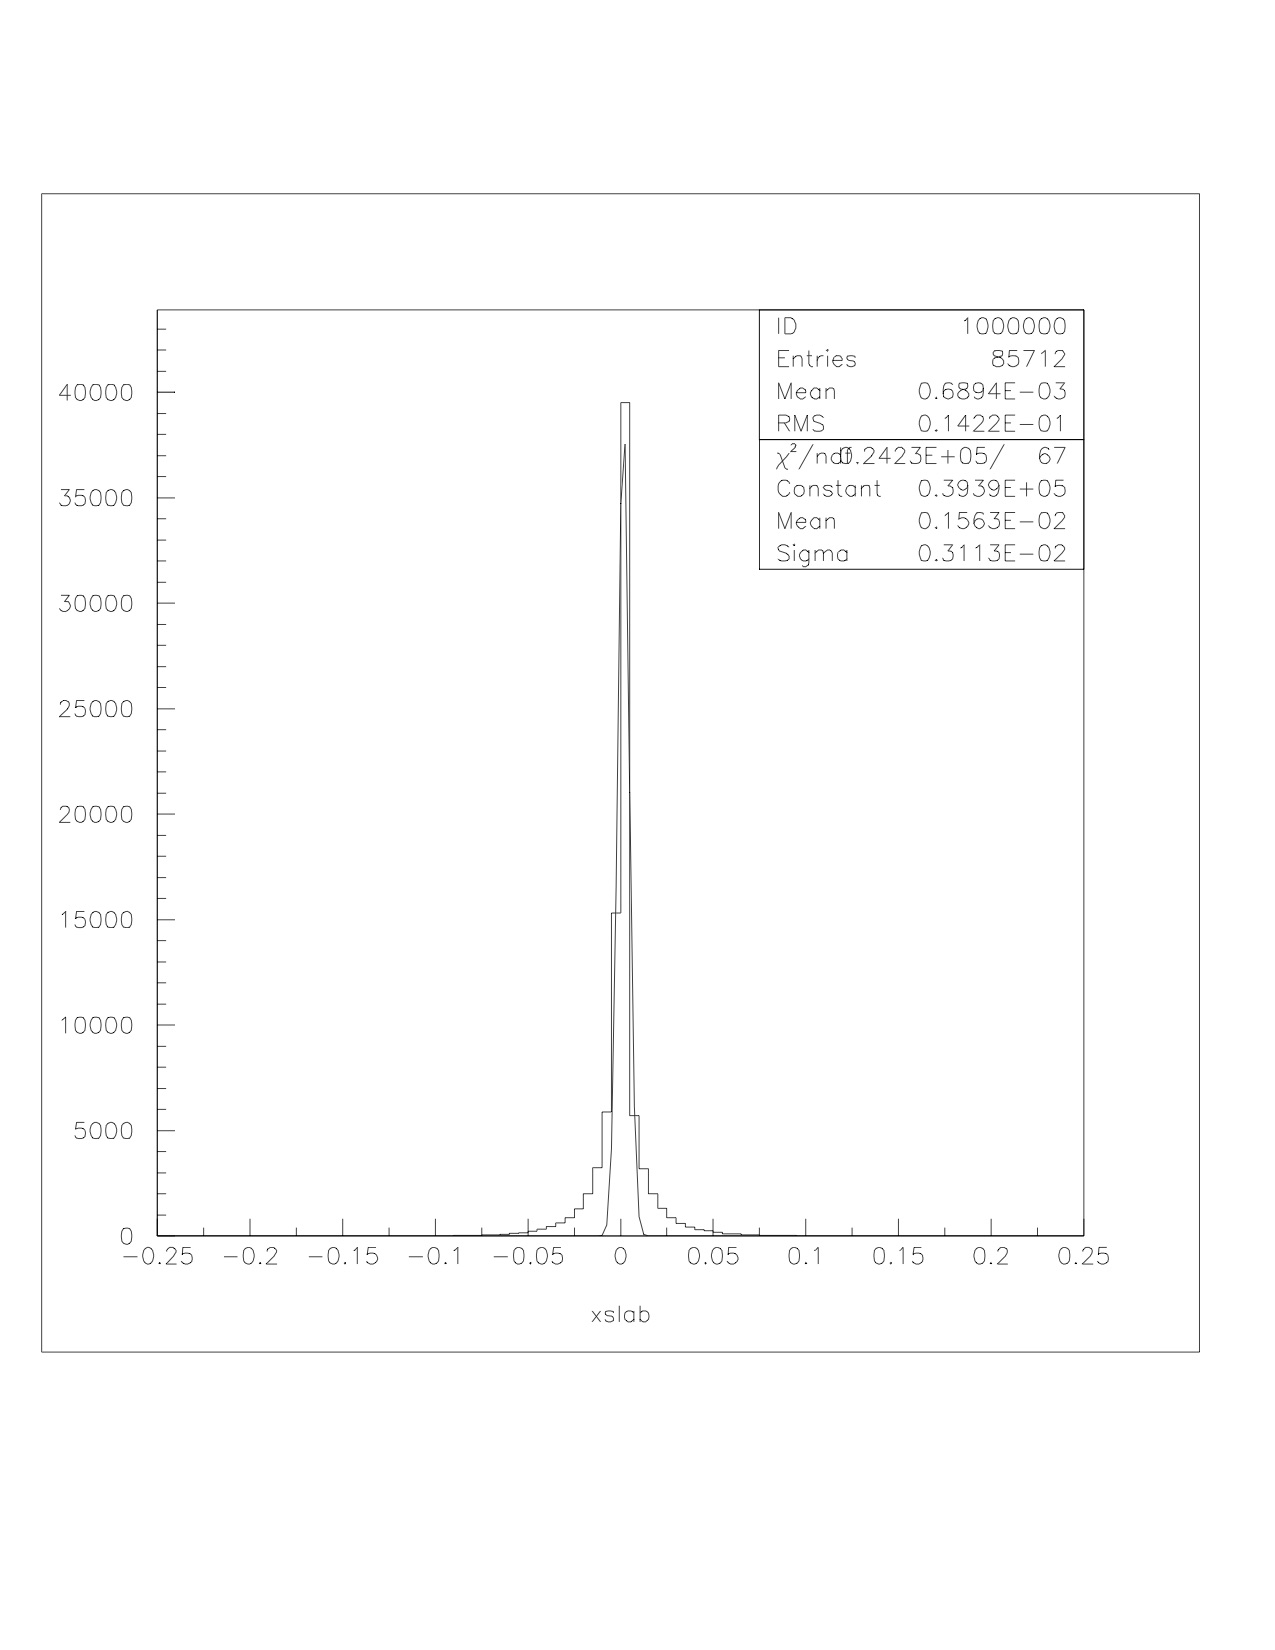
\includegraphics[width=0.45\textwidth]{ex_images/1_020_050_xs.jpg}}
  \subfloat[][$\gamma$ energy $=$ 140 KeV] {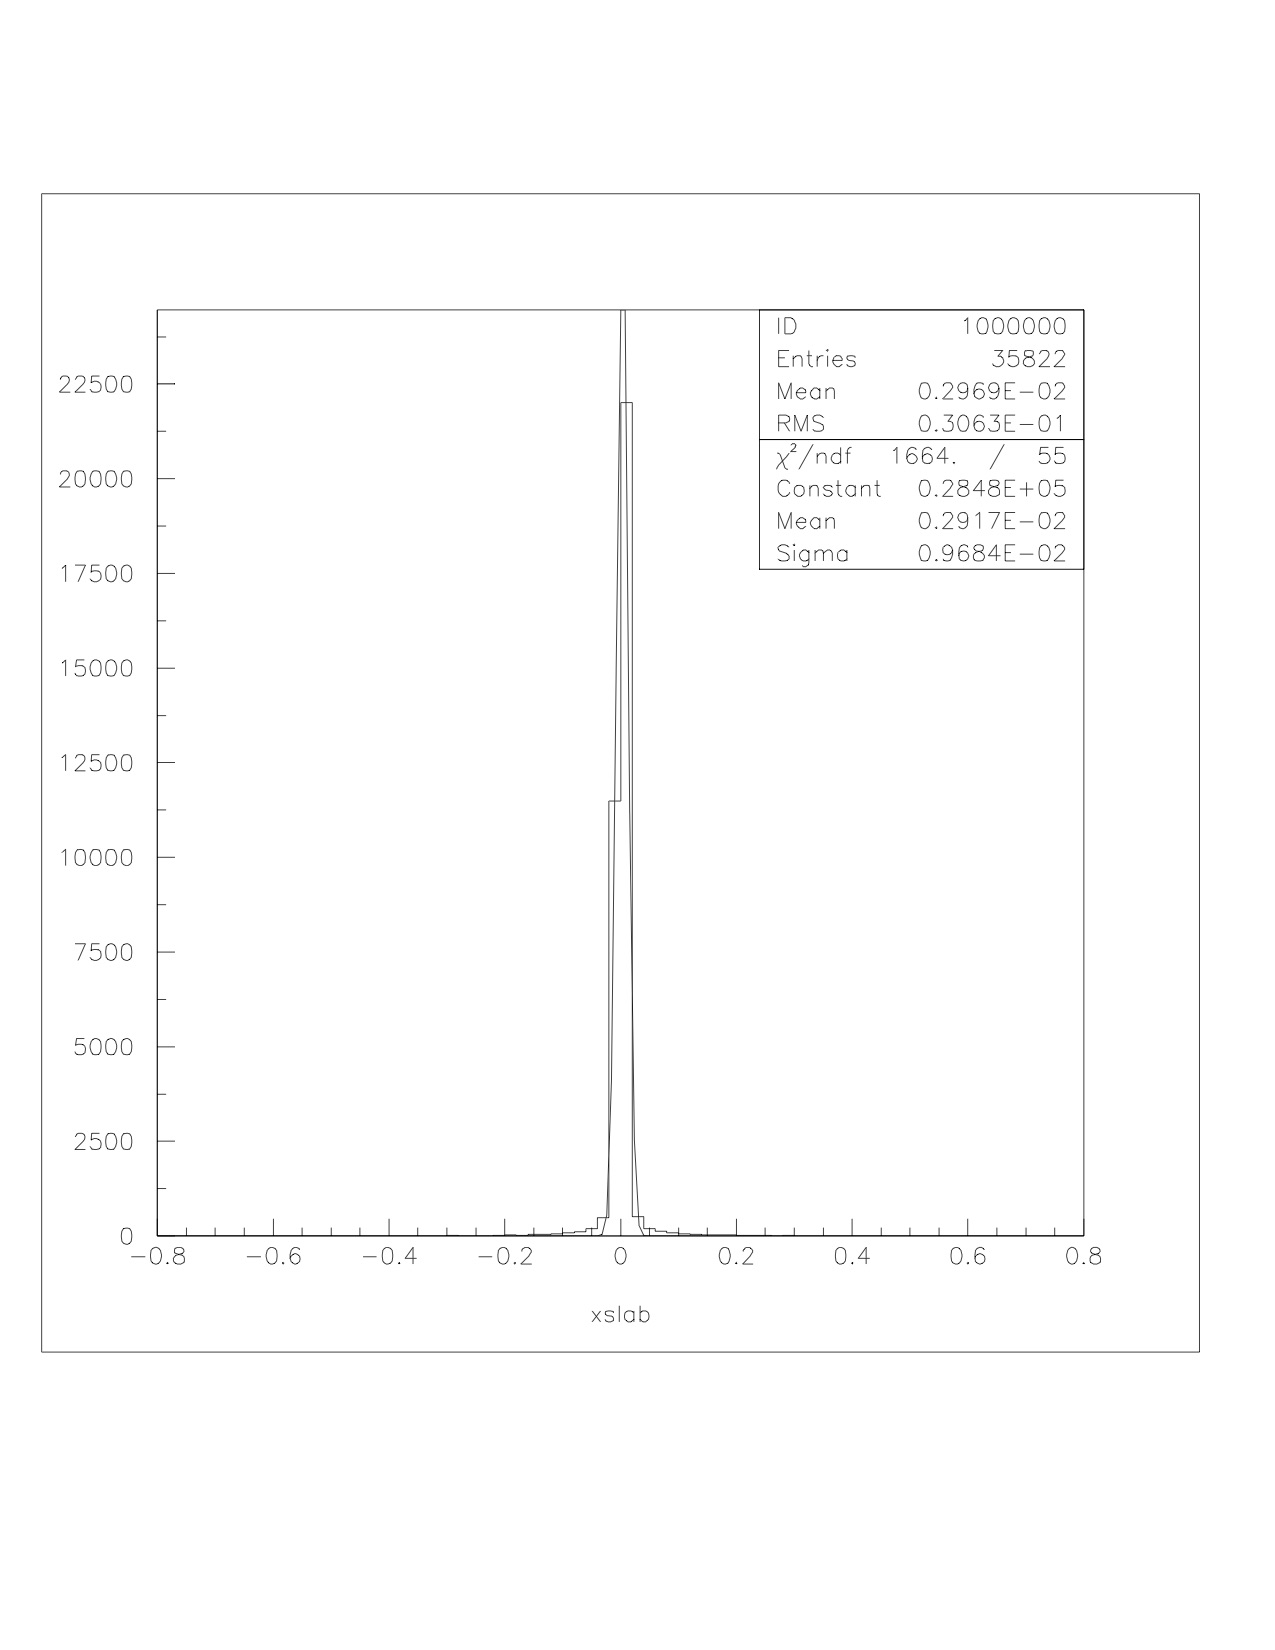
\includegraphics[width=0.45\textwidth]{ex_images/1_020_140_xs.jpg}}
  \caption{PSF plots with detector thickness of 2 mm, no blur.}
  \label{fig:020_xs}
\end{figure}

\begin{figure}[H]
  \centering
  \subfloat[][$\gamma$ energy $=$ 10 KeV] {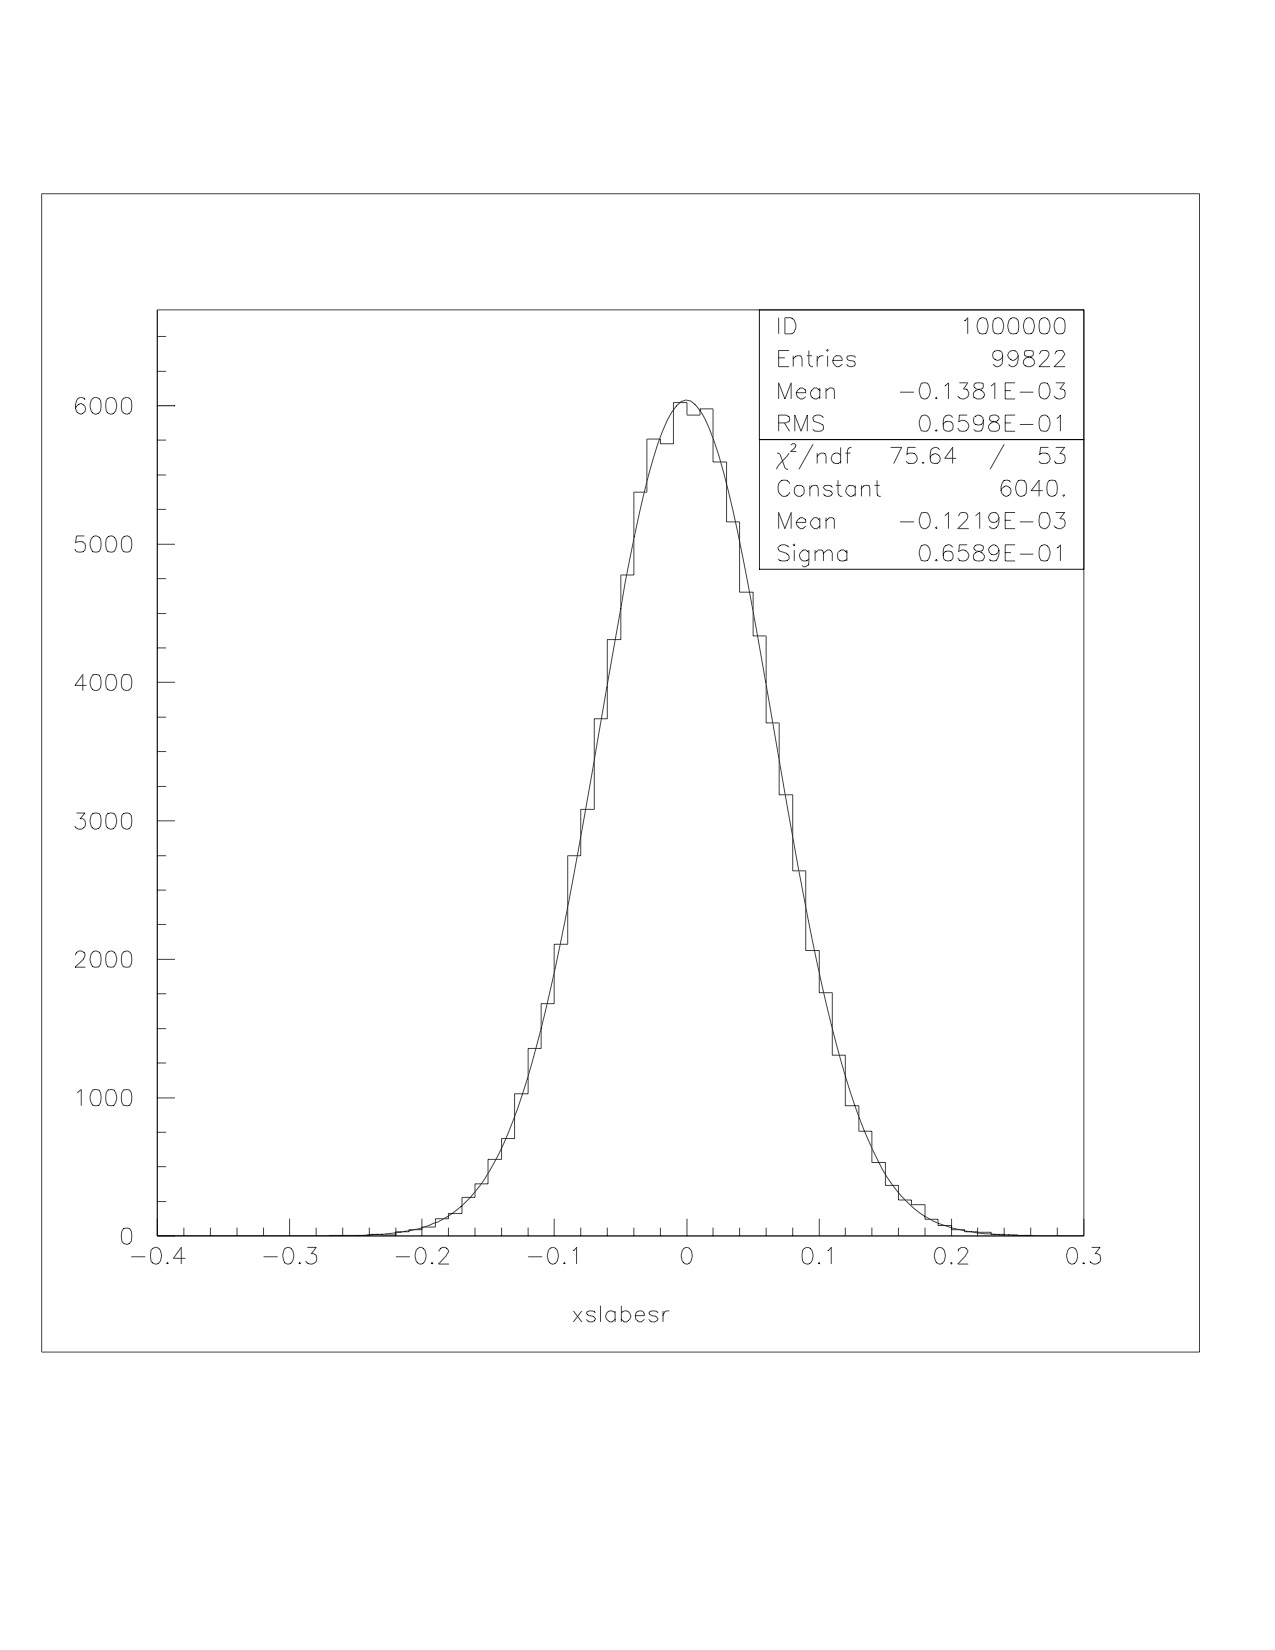
\includegraphics[width=0.45\textwidth]{ex_images/1_020_010_xse.jpg}}
  \subfloat[][$\gamma$ energy $=$ 30 KeV] {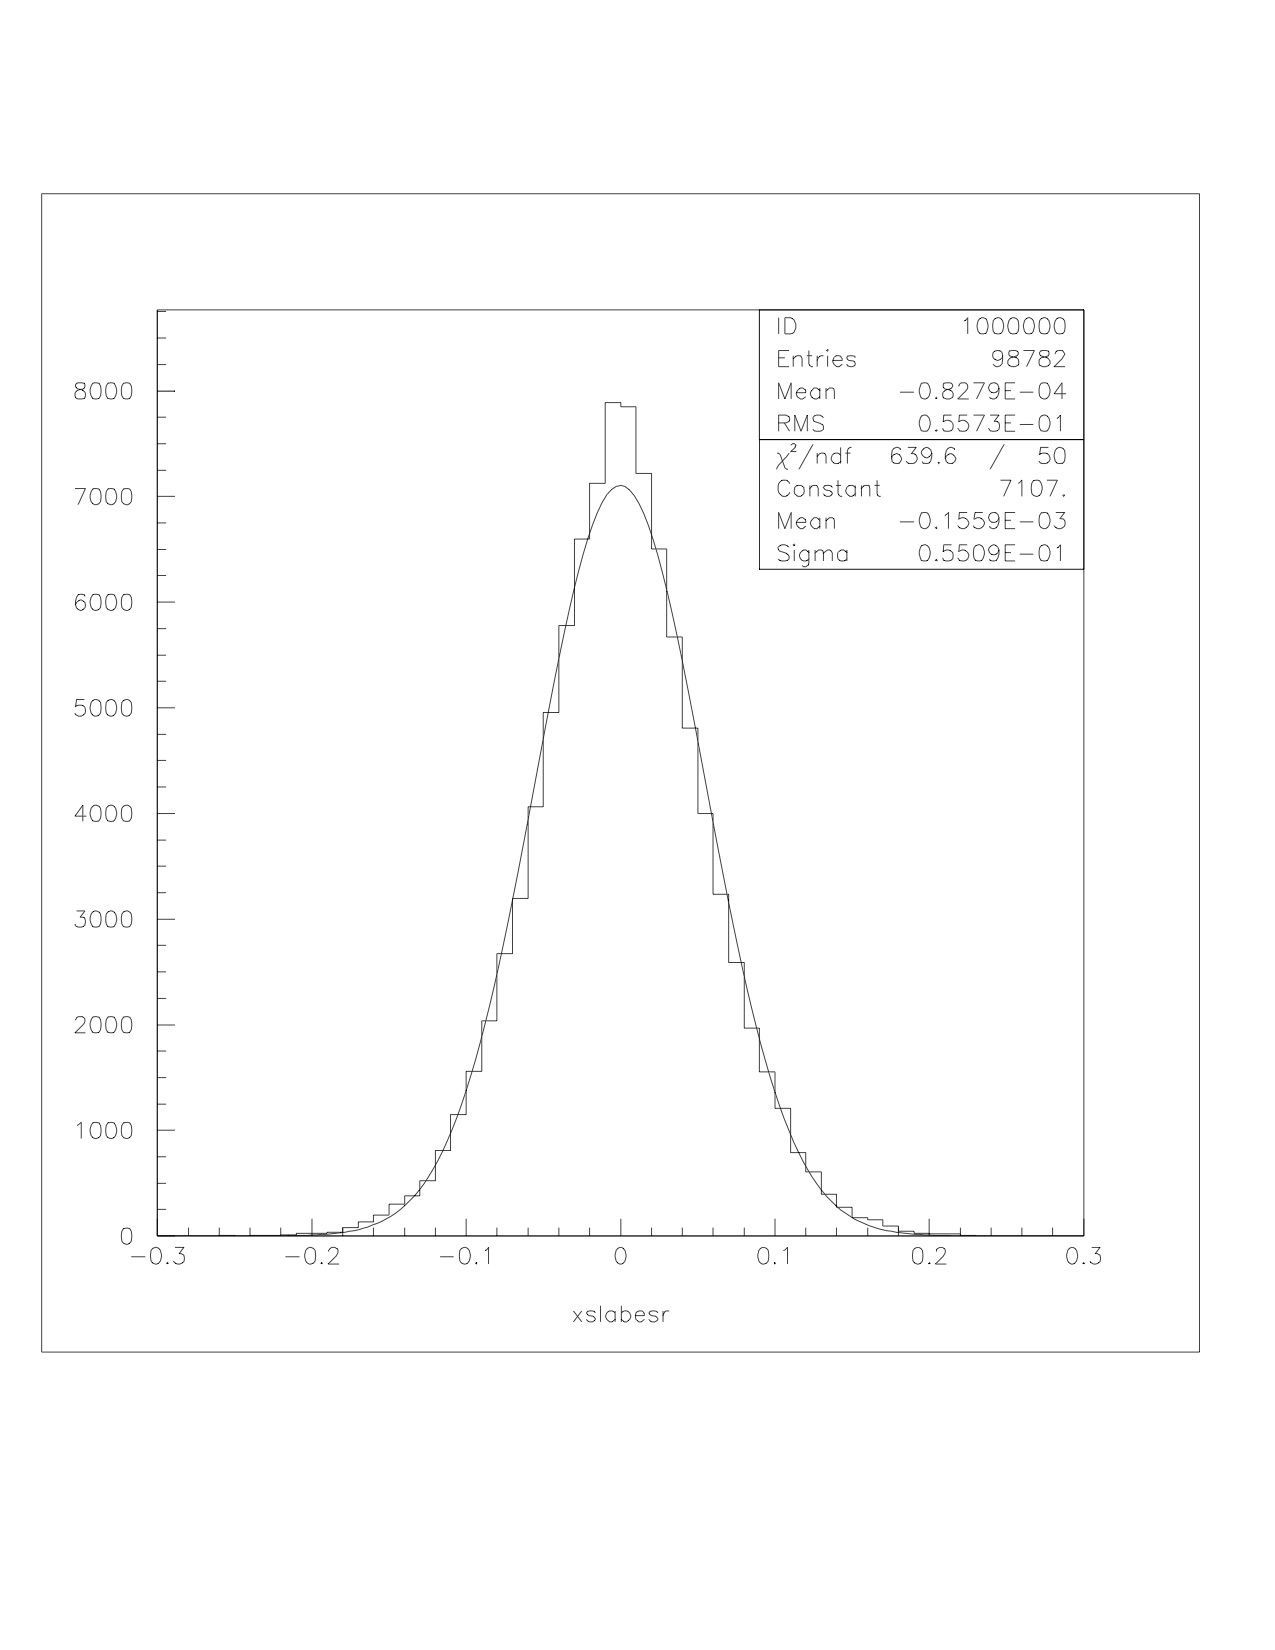
\includegraphics[width=0.45\textwidth]{ex_images/1_020_030_xse.jpg}}\\
  \subfloat[][$\gamma$ energy $=$ 50 KeV] {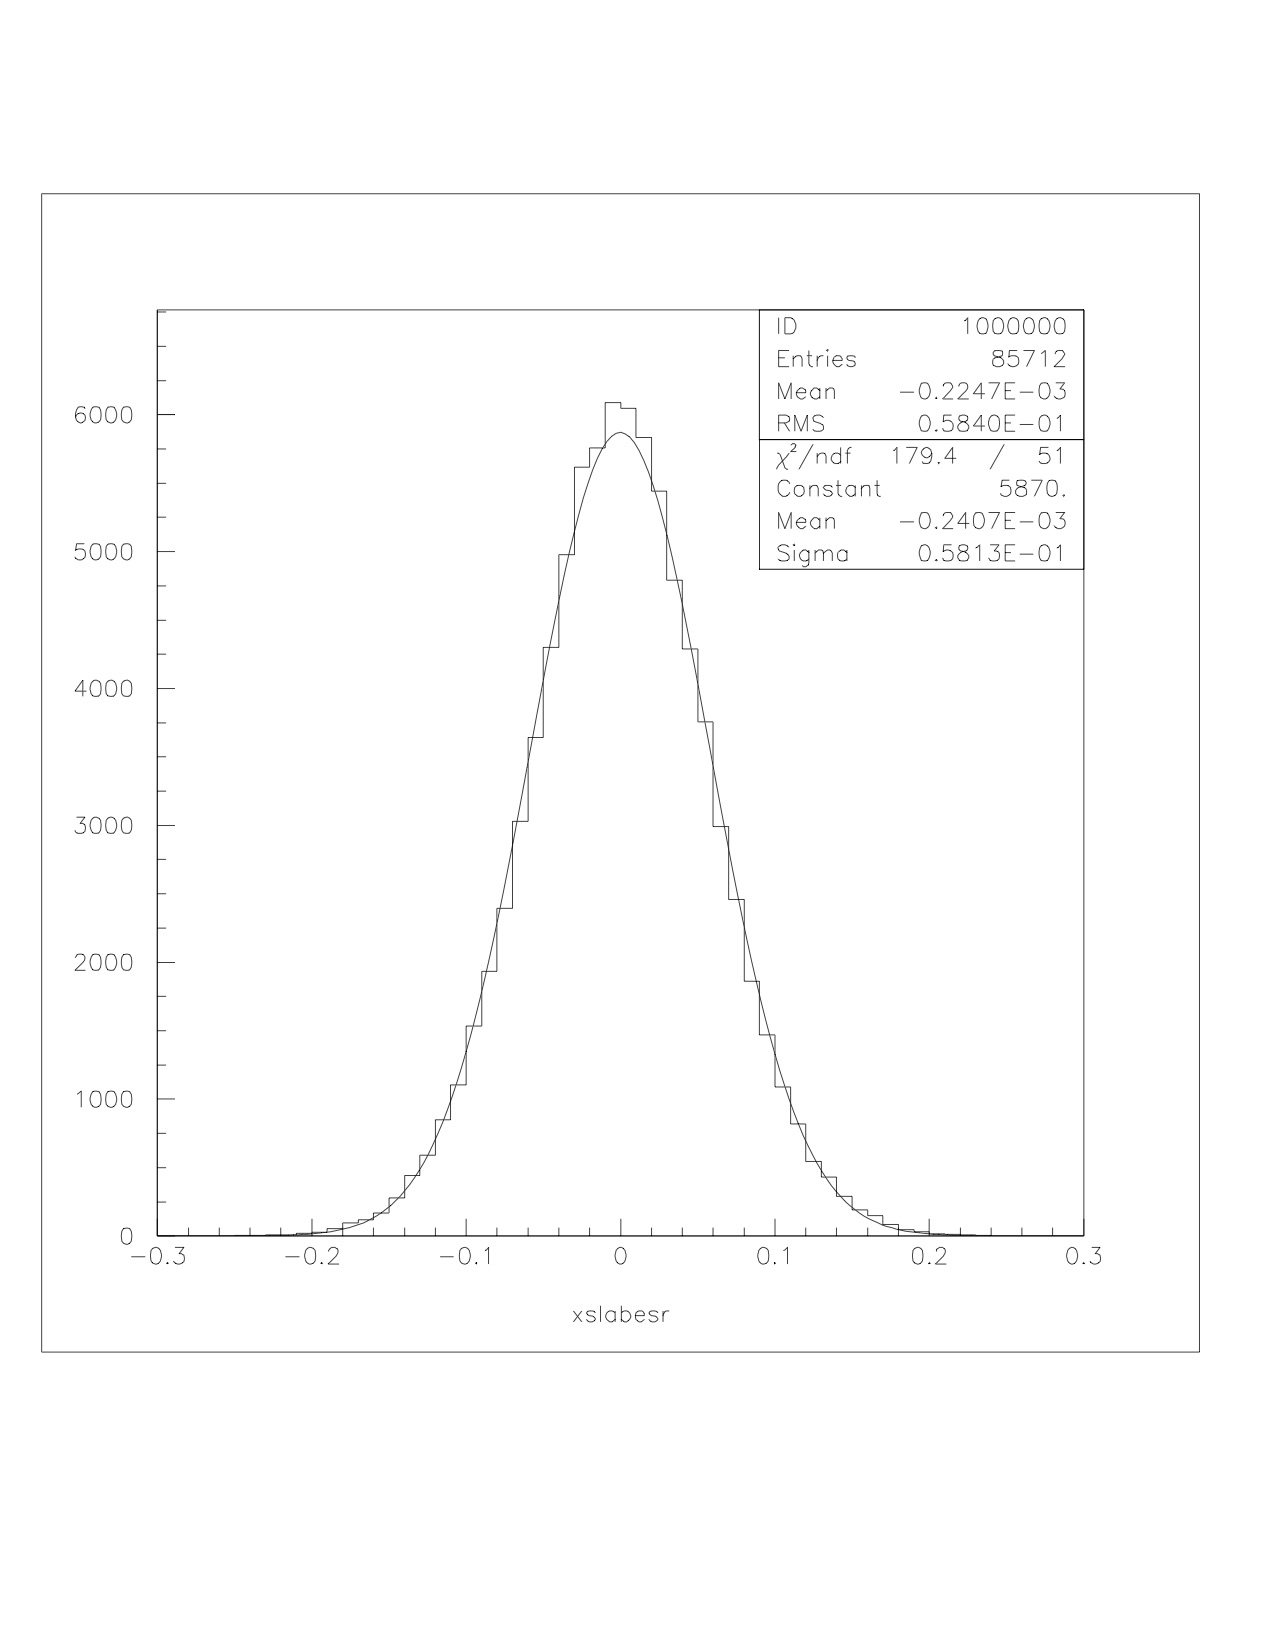
\includegraphics[width=0.45\textwidth]{ex_images/1_020_050_xse.jpg}}
  \subfloat[][$\gamma$ energy $=$ 140 KeV] {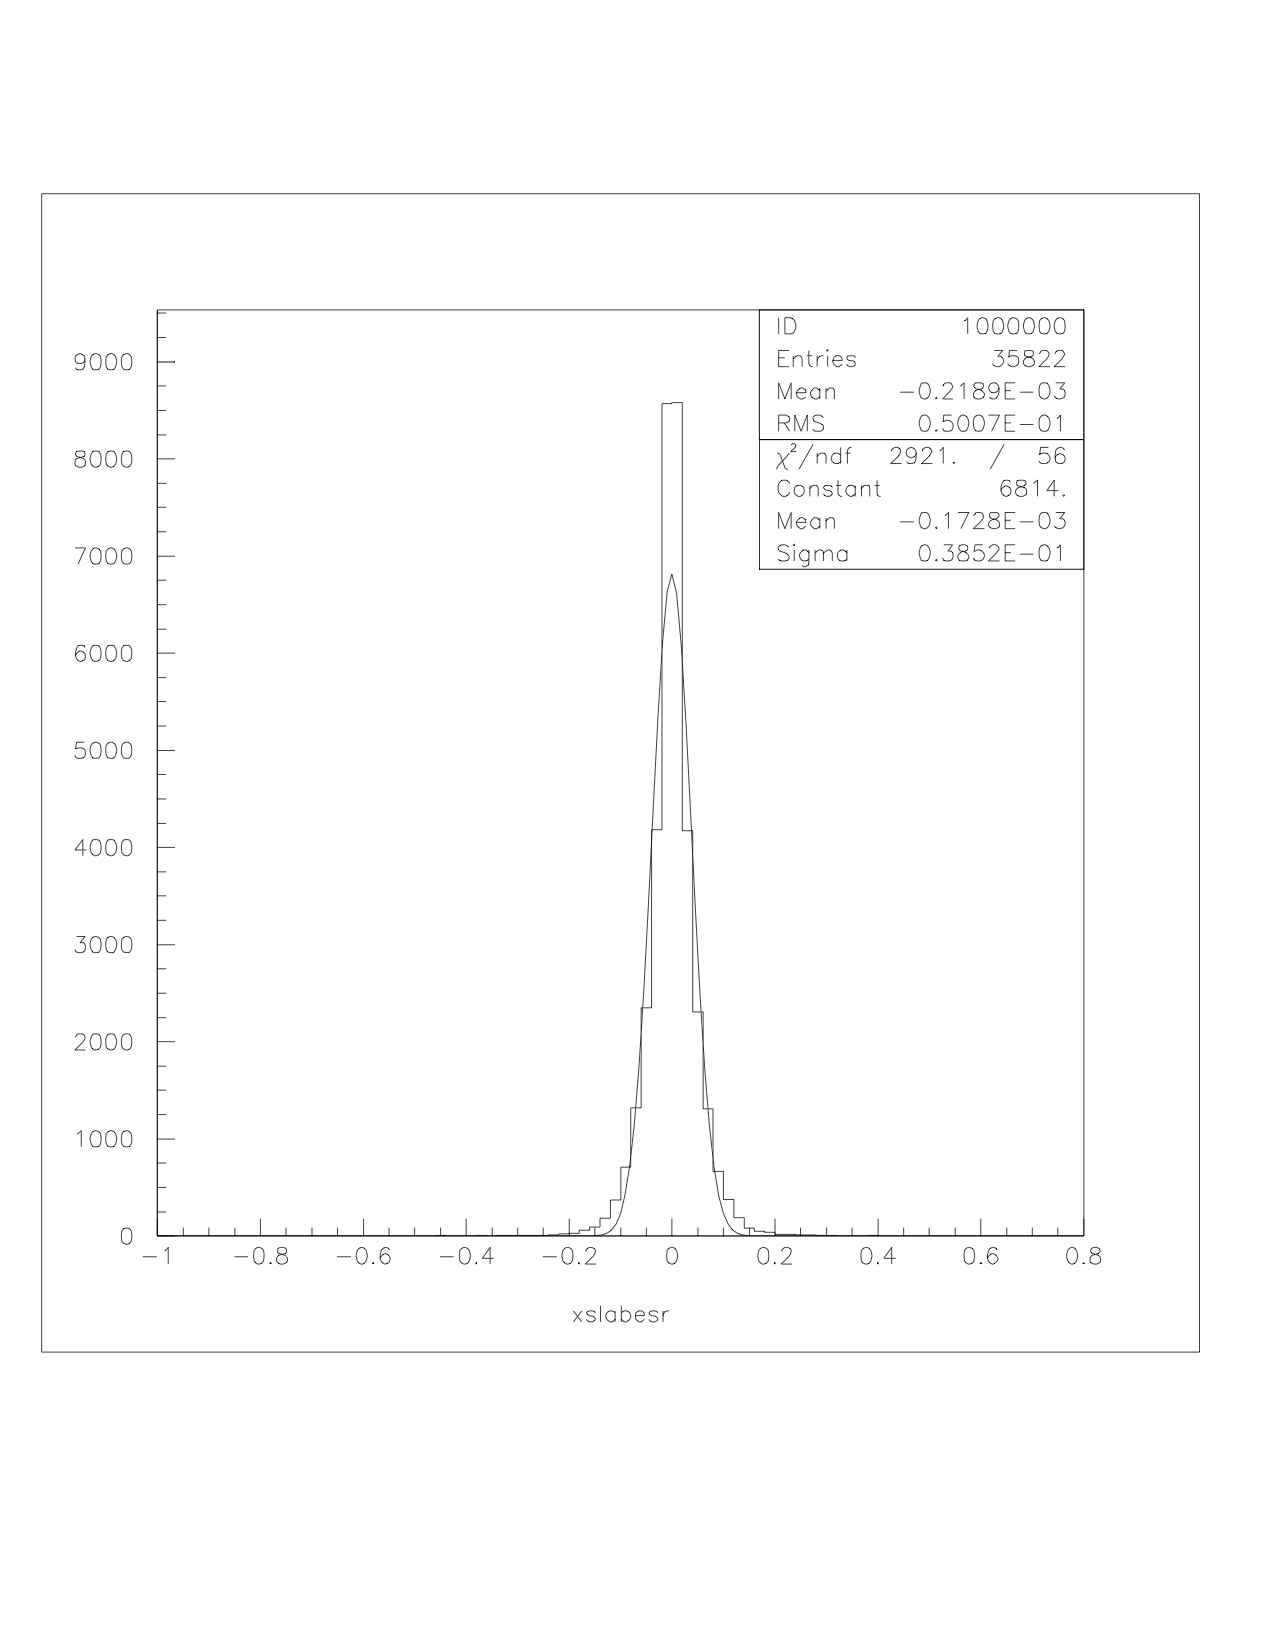
\includegraphics[width=0.45\textwidth]{ex_images/1_020_140_xse.jpg}}
  \caption{PSF plots with detector thickness of 2 mm, with blur.}
  \label{fig:020_xse}
\end{figure}

\begin{figure}[H]
  \centering
  \subfloat[][$\gamma$ energy $=$ 10 KeV] {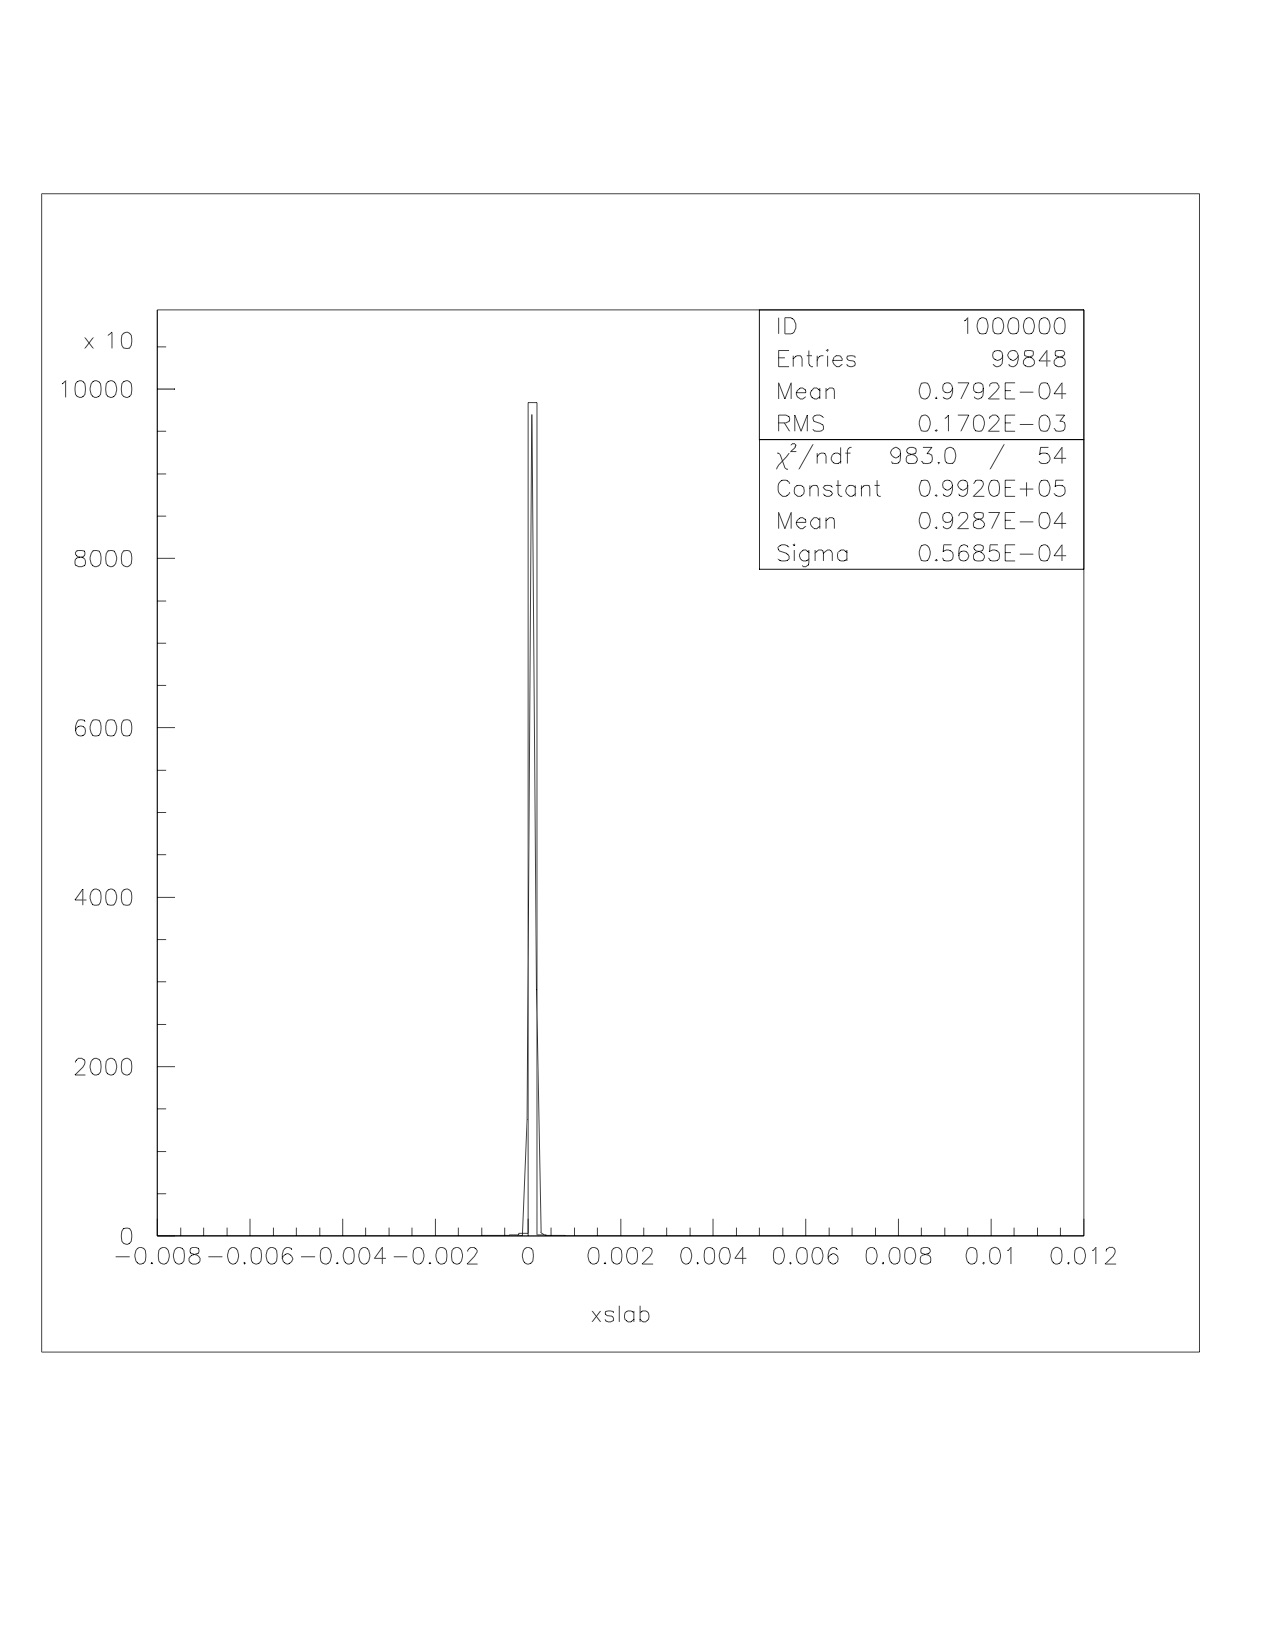
\includegraphics[width=0.45\textwidth]{ex_images/1_050_010_xs.jpg}}
  \subfloat[][$\gamma$ energy $=$ 30 KeV] {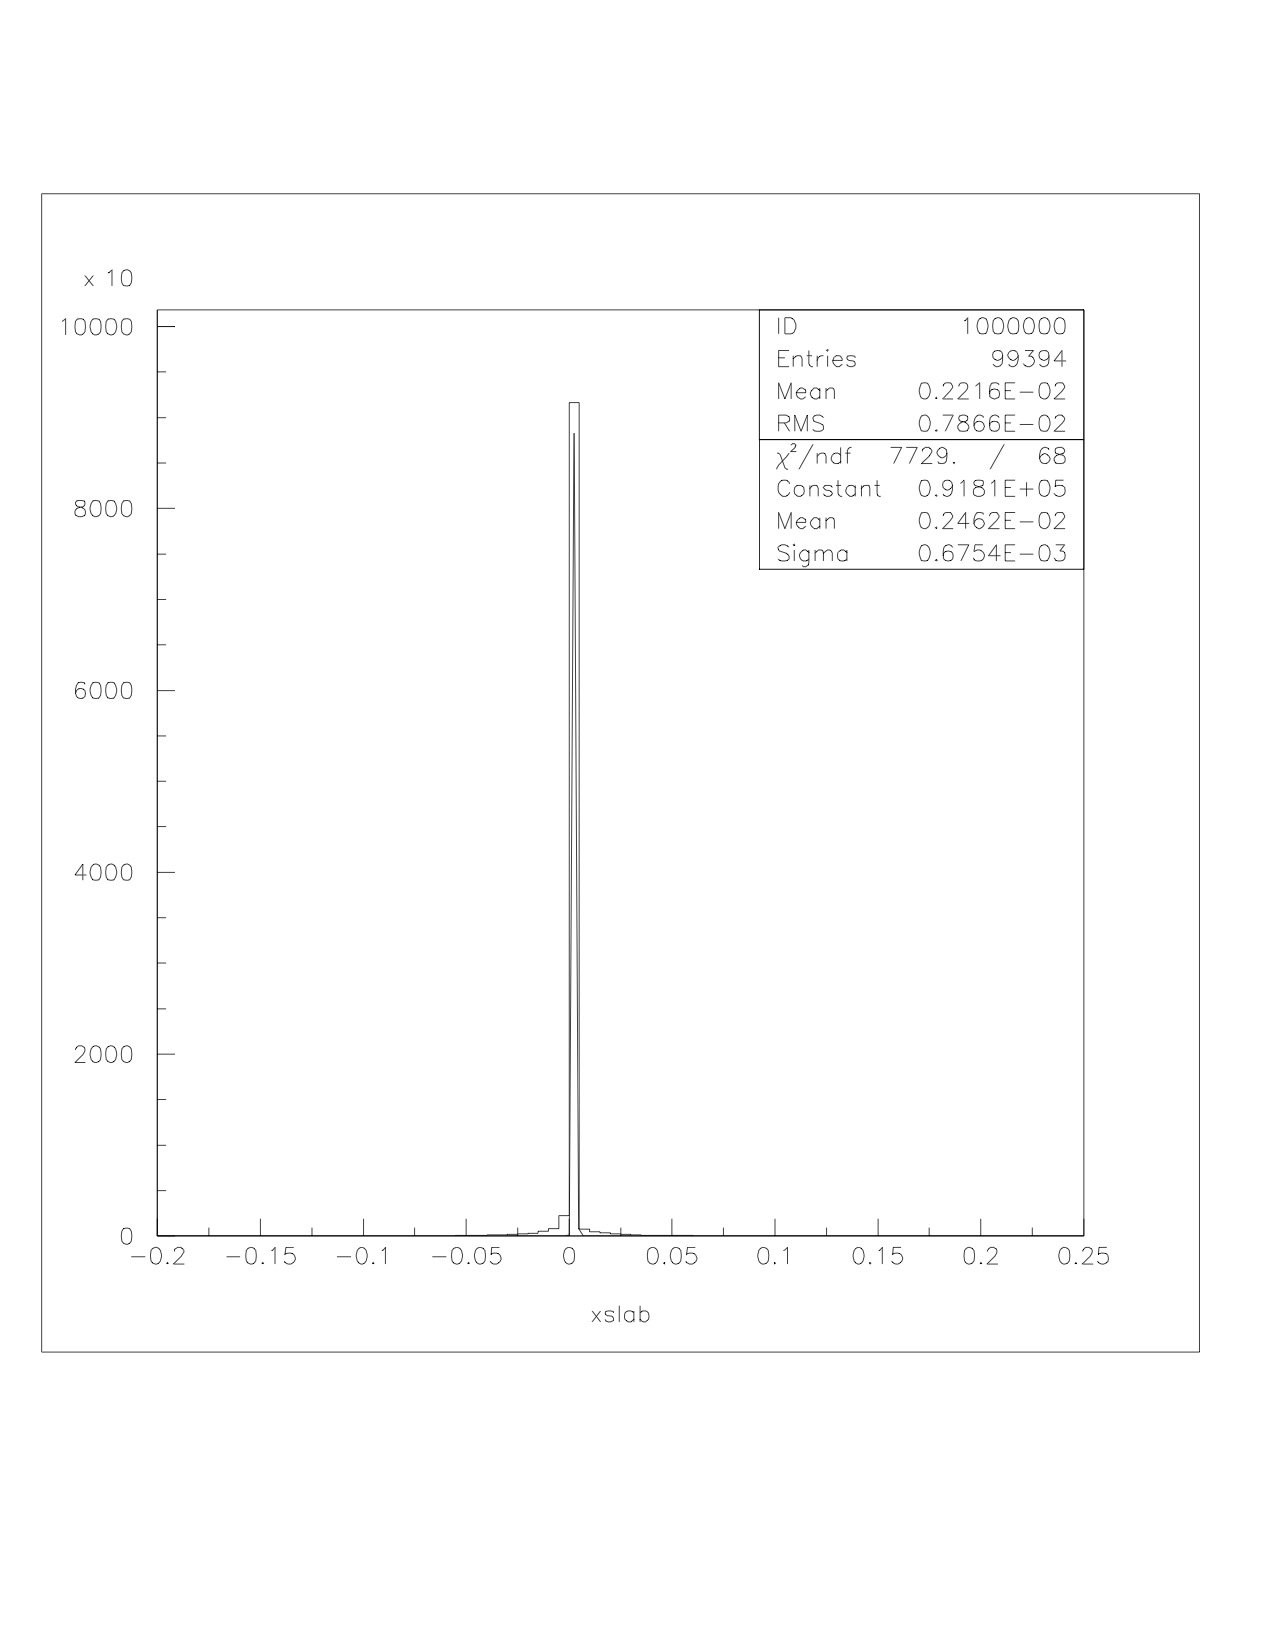
\includegraphics[width=0.45\textwidth]{ex_images/1_050_030_xs.jpg}}\\
  \subfloat[][$\gamma$ energy $=$ 50 KeV] {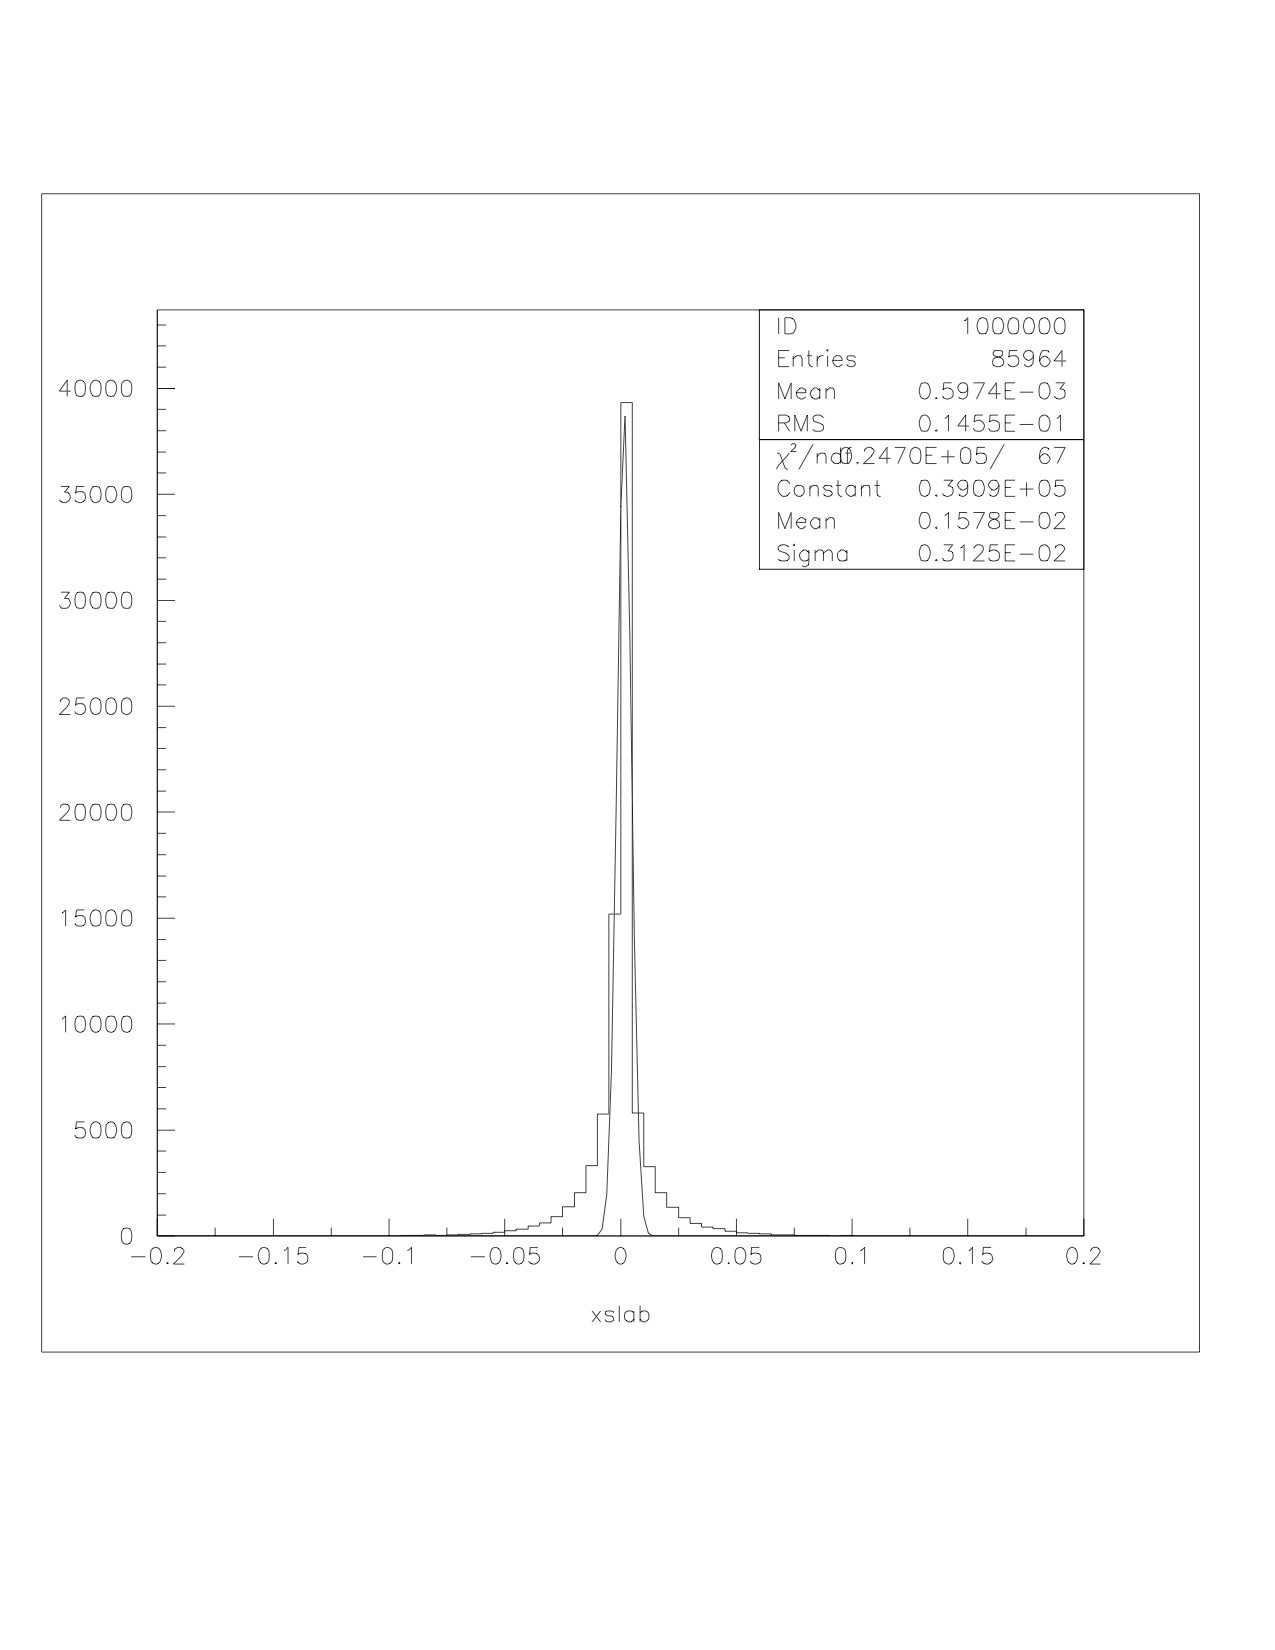
\includegraphics[width=0.45\textwidth]{ex_images/1_050_050_xs.jpg}}
  \subfloat[][$\gamma$ energy $=$ 140 KeV] {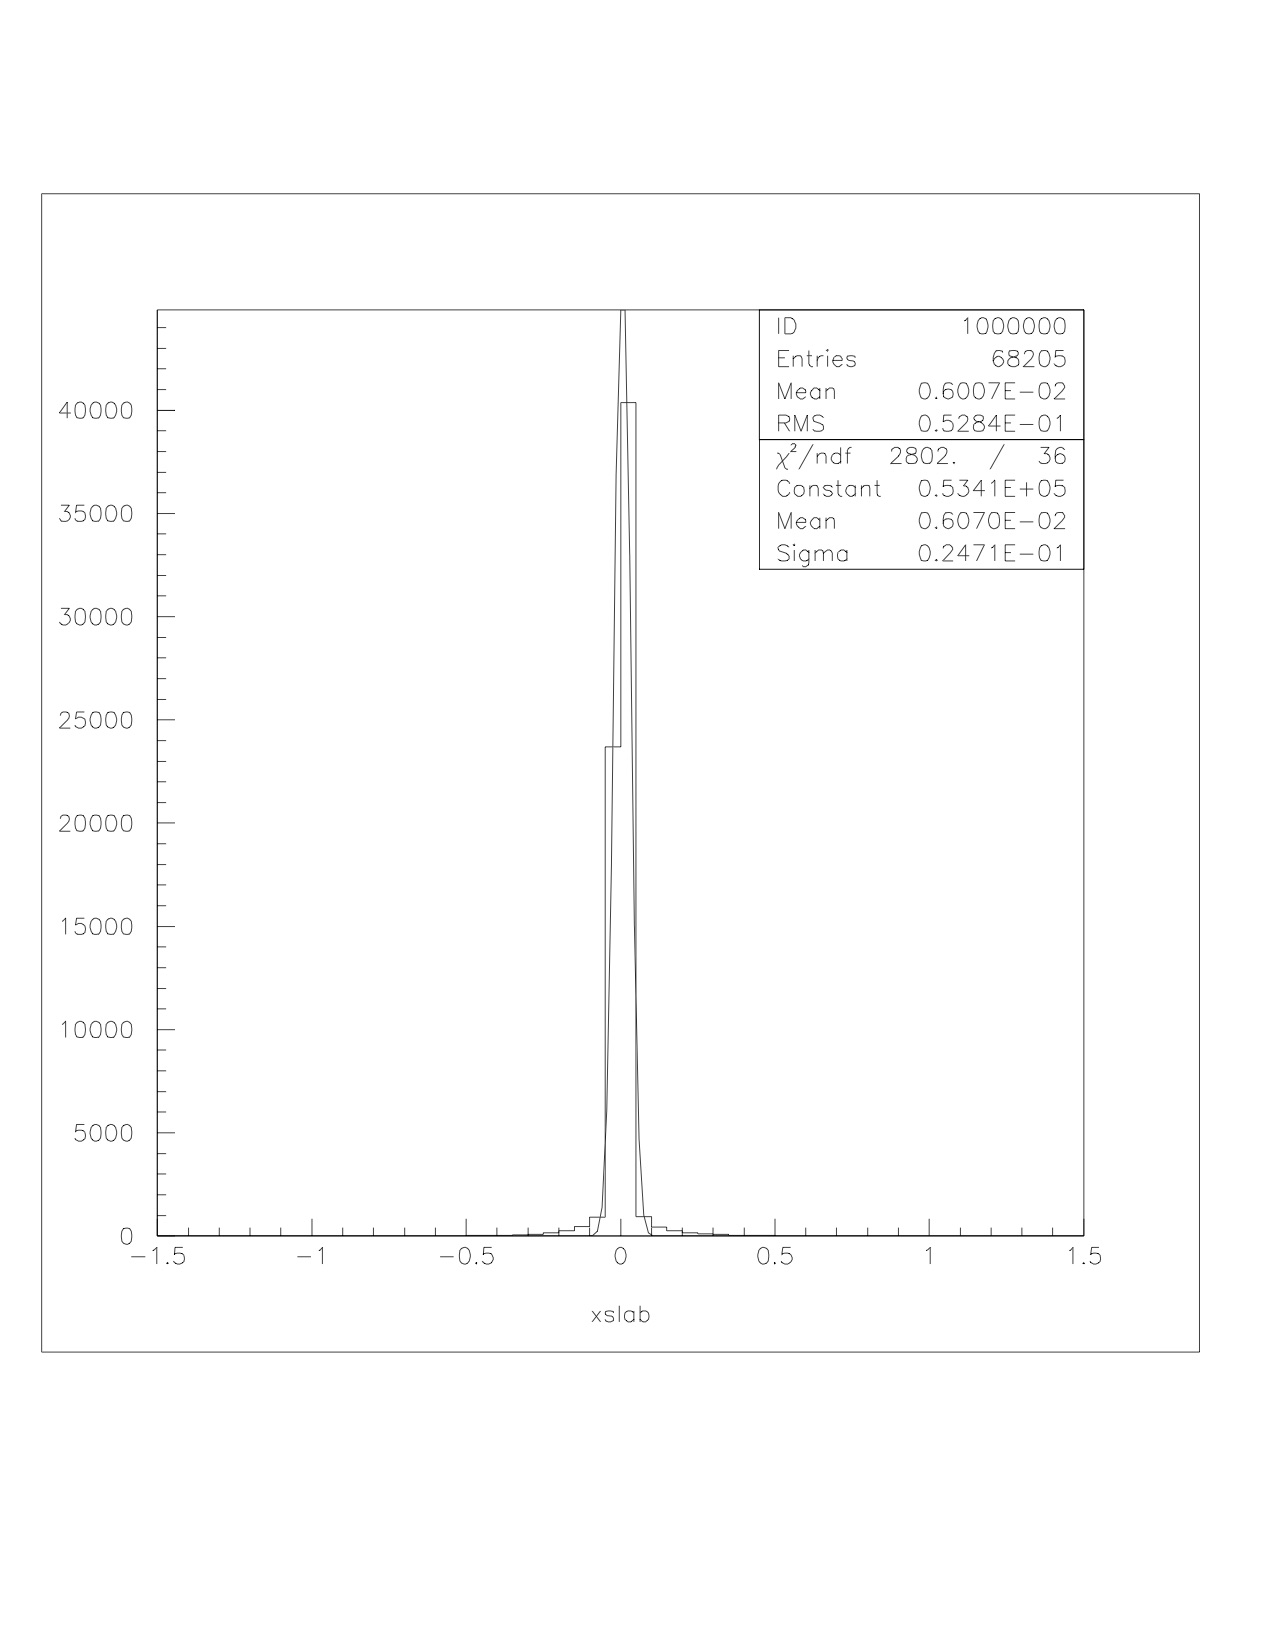
\includegraphics[width=0.45\textwidth]{ex_images/1_050_140_xs.jpg}}
  \caption{PSF plots with detector thickness of 5 mm, no blur.}
  \label{fig:050_xs}
\end{figure}

\begin{figure}[H]
  \centering
  \subfloat[][$\gamma$ energy $=$ 10 KeV] {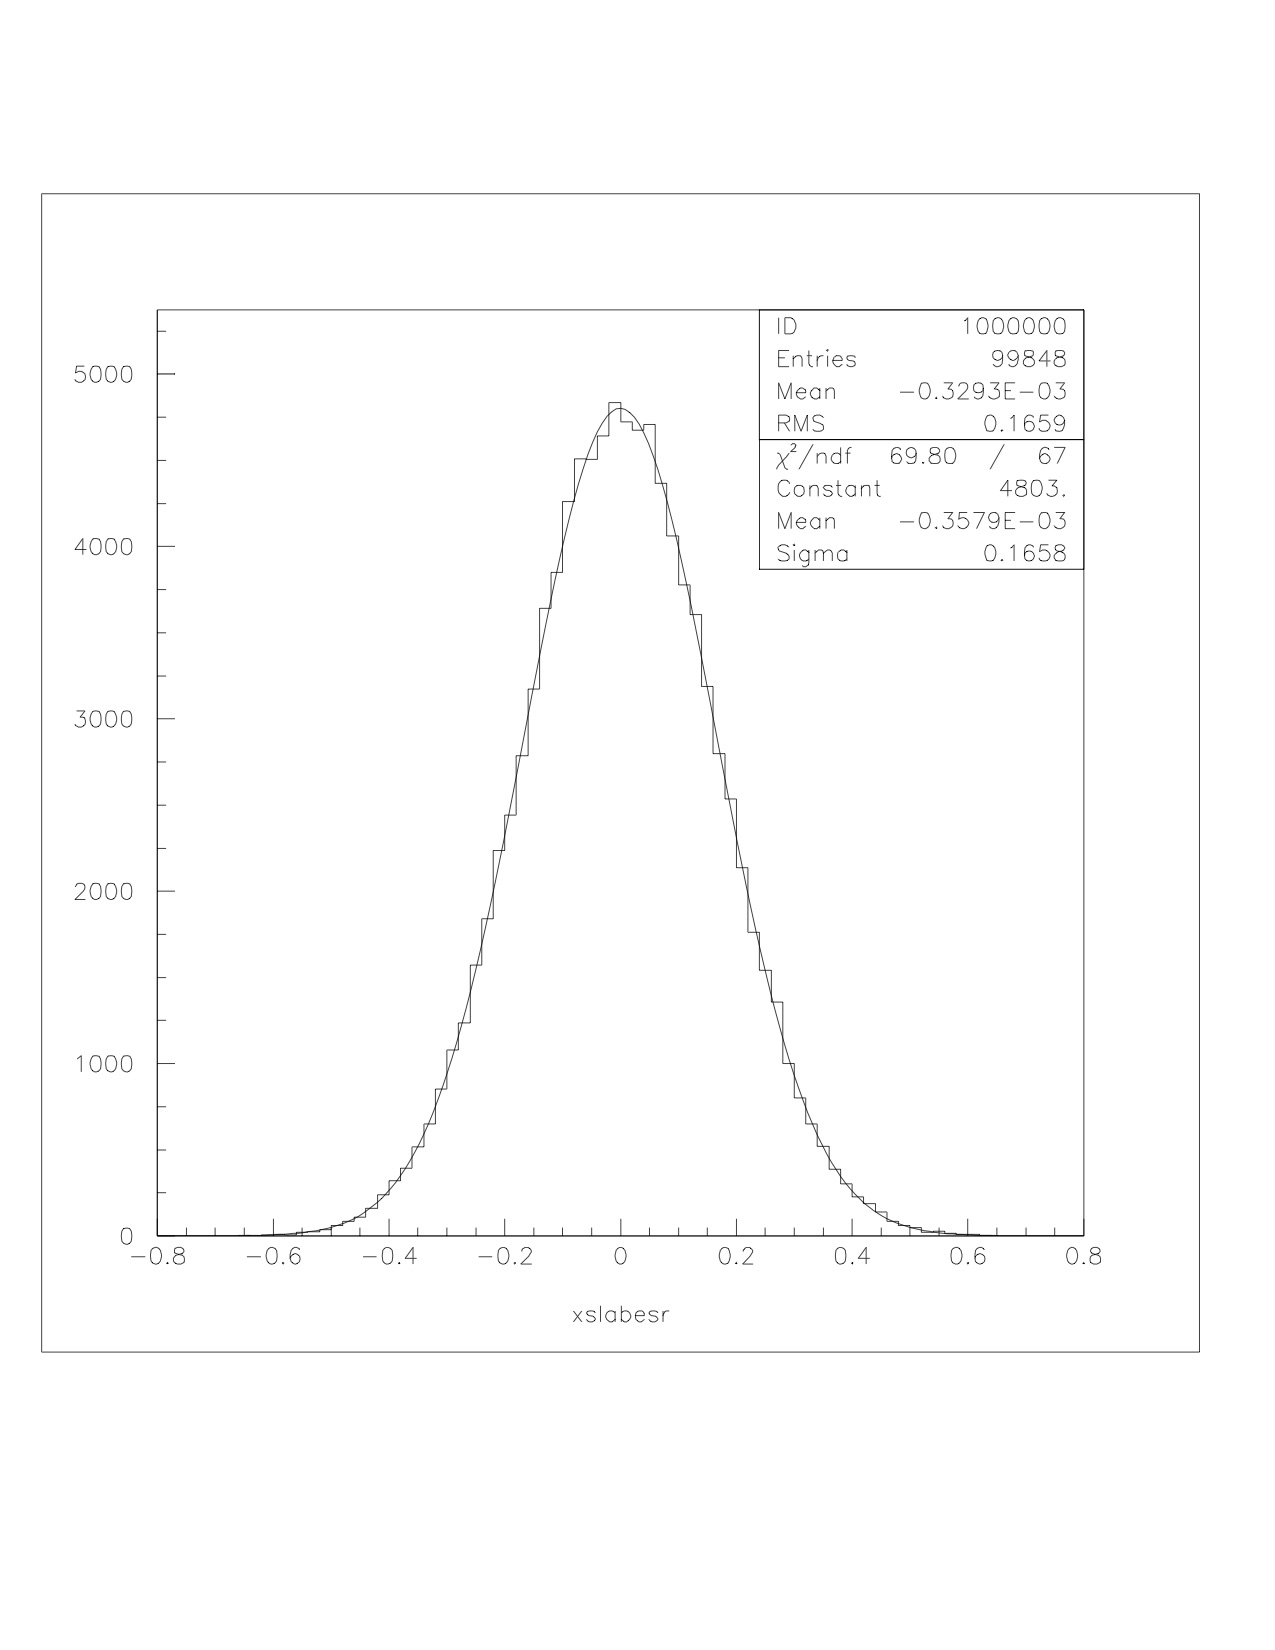
\includegraphics[width=0.45\textwidth]{ex_images/1_050_010_xse.jpg}}
  \subfloat[][$\gamma$ energy $=$ 30 KeV] {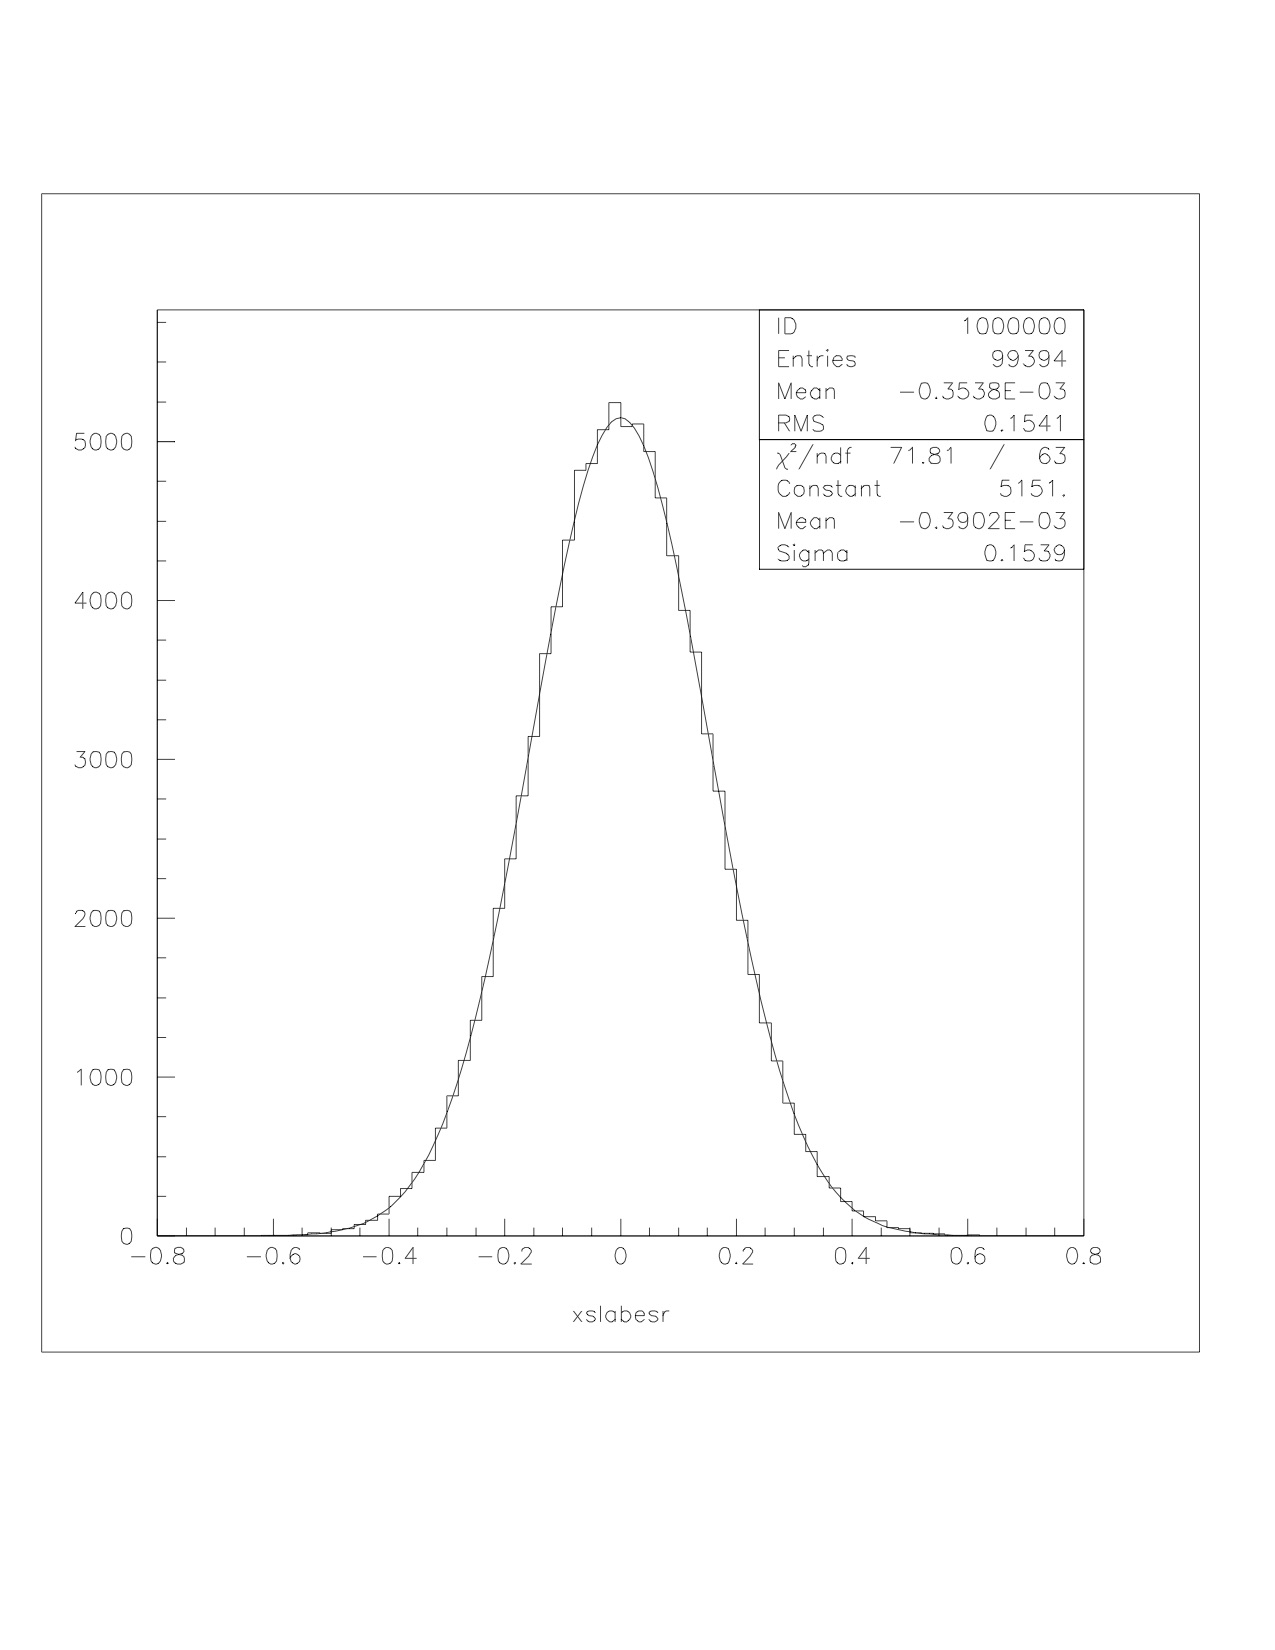
\includegraphics[width=0.45\textwidth]{ex_images/1_050_030_xse.jpg}}\\
  \subfloat[][$\gamma$ energy $=$ 50 KeV] {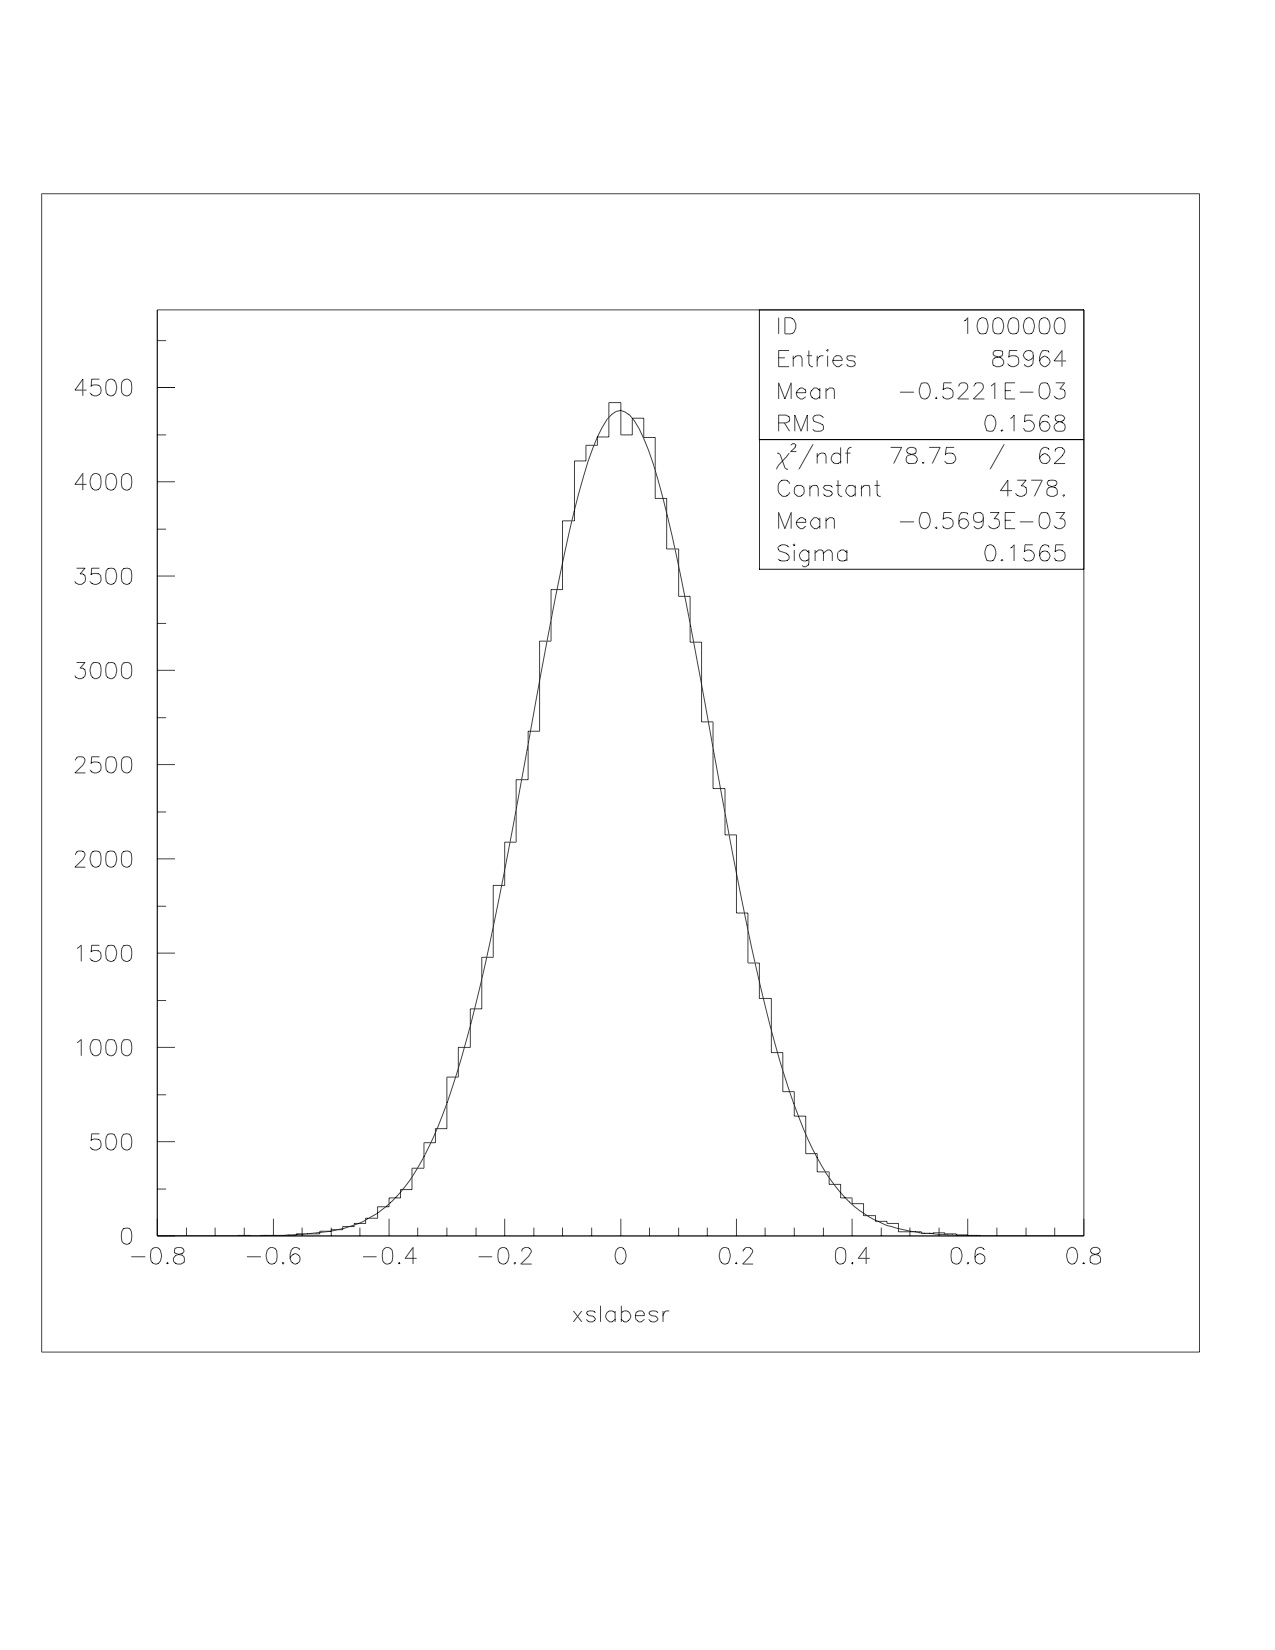
\includegraphics[width=0.45\textwidth]{ex_images/1_050_050_xse.jpg}}
  \subfloat[][$\gamma$ energy $=$ 140 KeV] {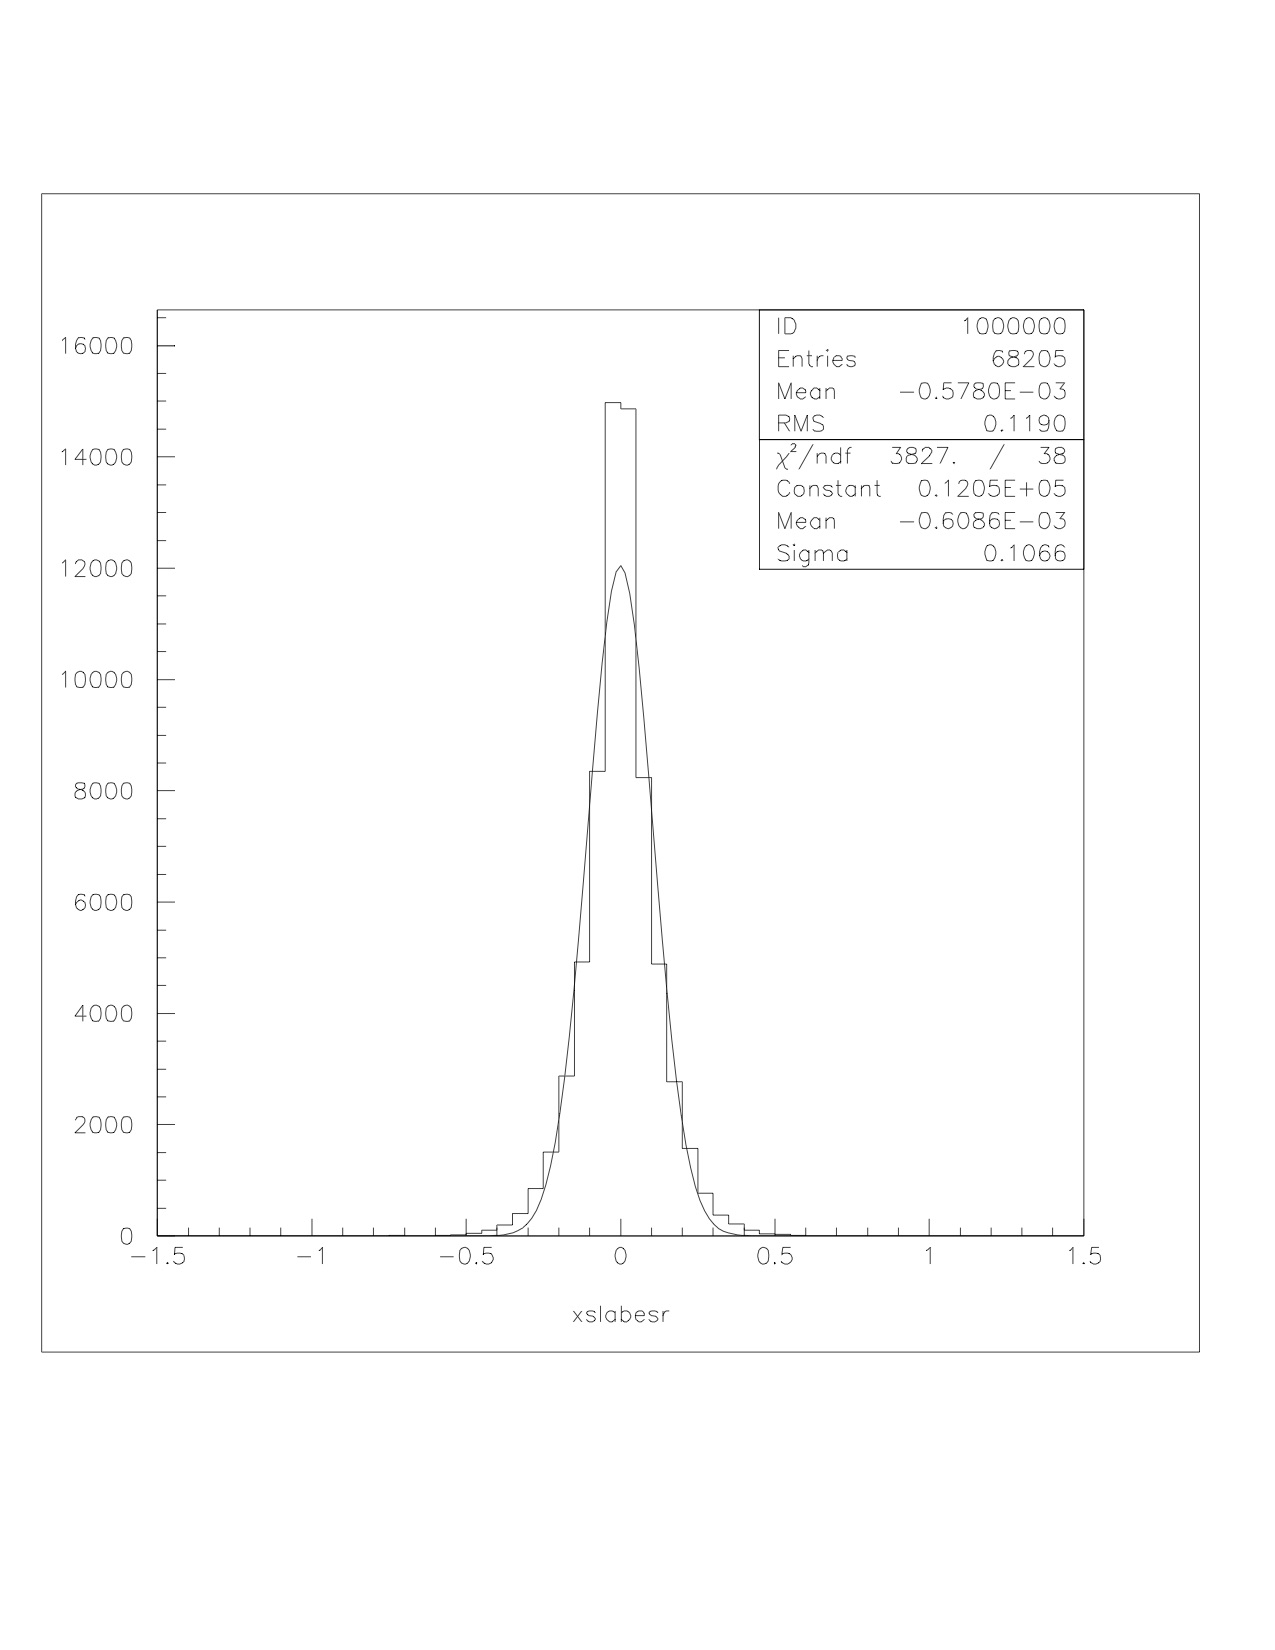
\includegraphics[width=0.45\textwidth]{ex_images/1_050_140_xse.jpg}}
  \caption{PSF plots with detector thickness of 5 mm, with blur.}
  \label{fig:050_xse}
\end{figure}

\begin{figure}[H]
  \centering
  \subfloat[][$\gamma$ energy $=$ 10 KeV] {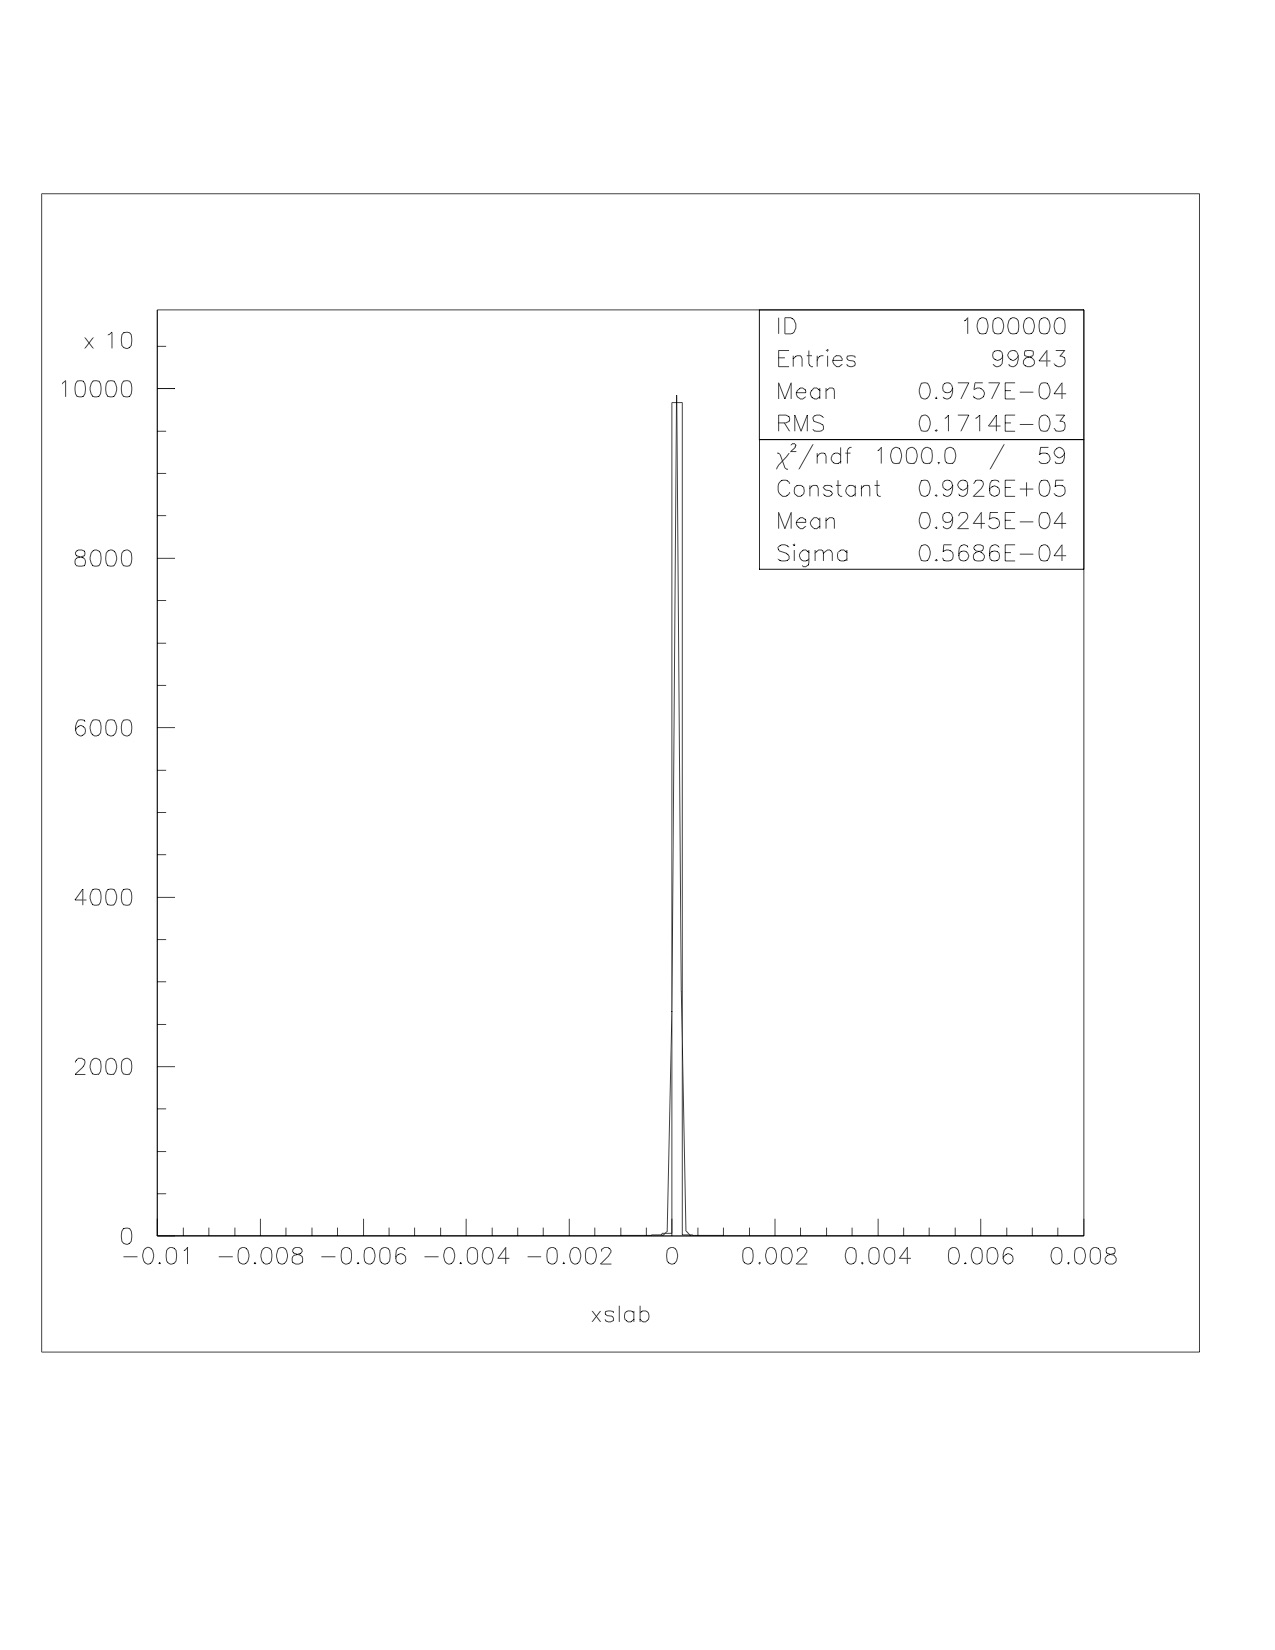
\includegraphics[width=0.45\textwidth]{ex_images/1_100_010_xs.jpg}}
  \subfloat[][$\gamma$ energy $=$ 30 KeV] {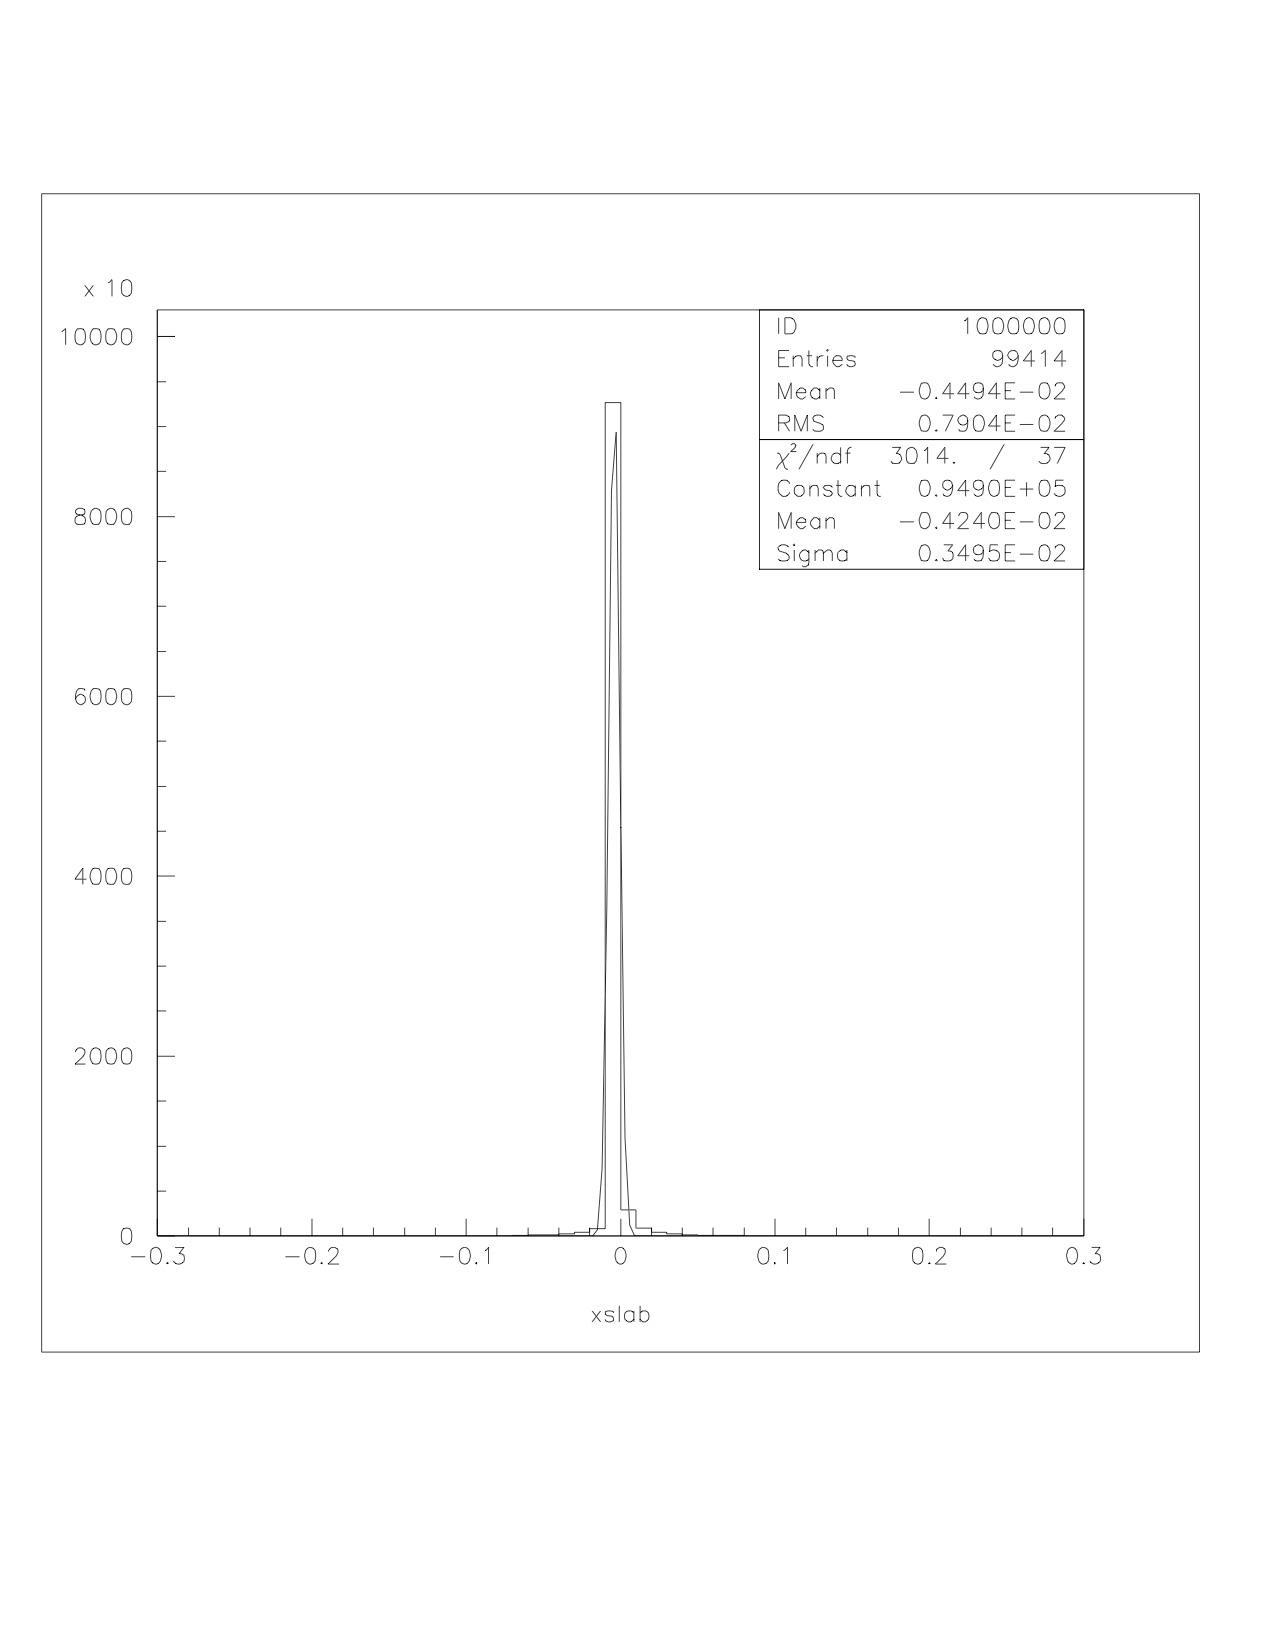
\includegraphics[width=0.45\textwidth]{ex_images/1_100_030_xs.jpg}}\\
  \subfloat[][$\gamma$ energy $=$ 50 KeV] {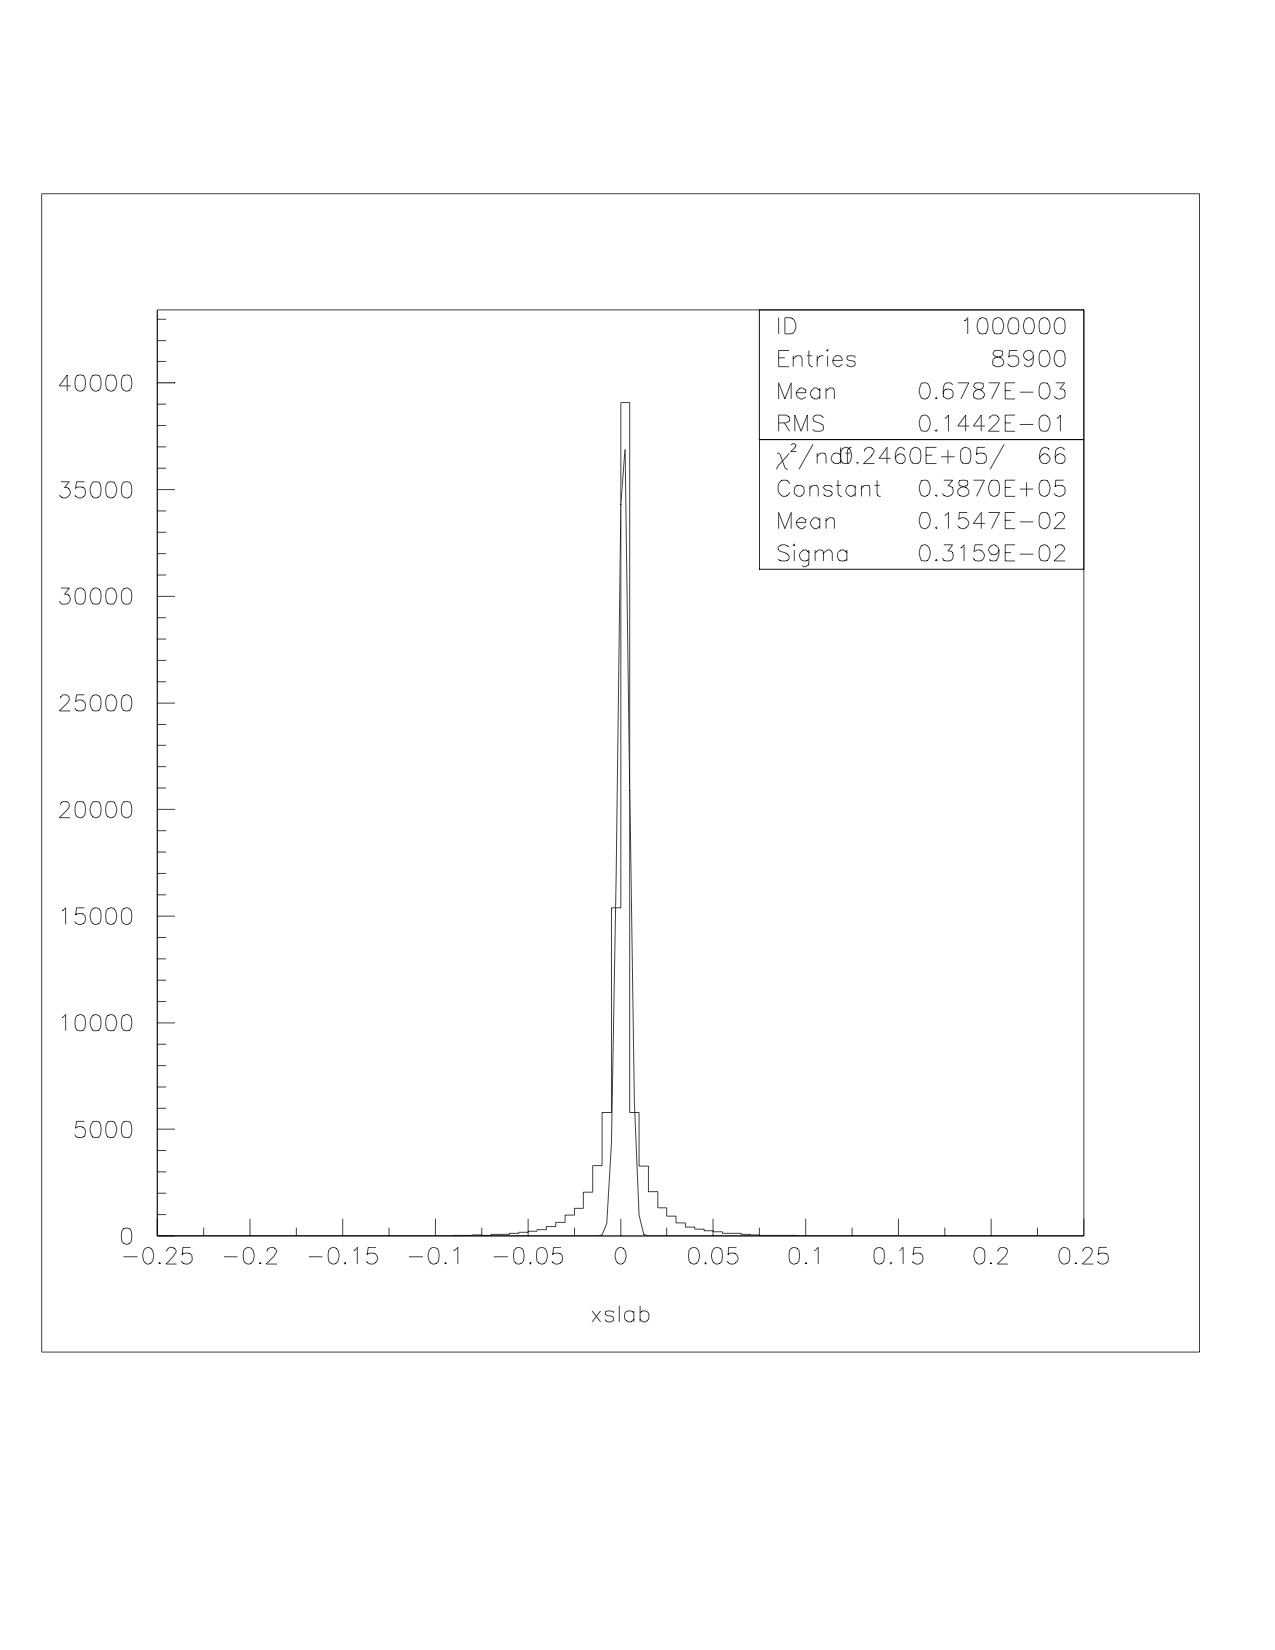
\includegraphics[width=0.45\textwidth]{ex_images/1_100_050_xs.jpg}}
  \subfloat[][$\gamma$ energy $=$ 140 KeV] {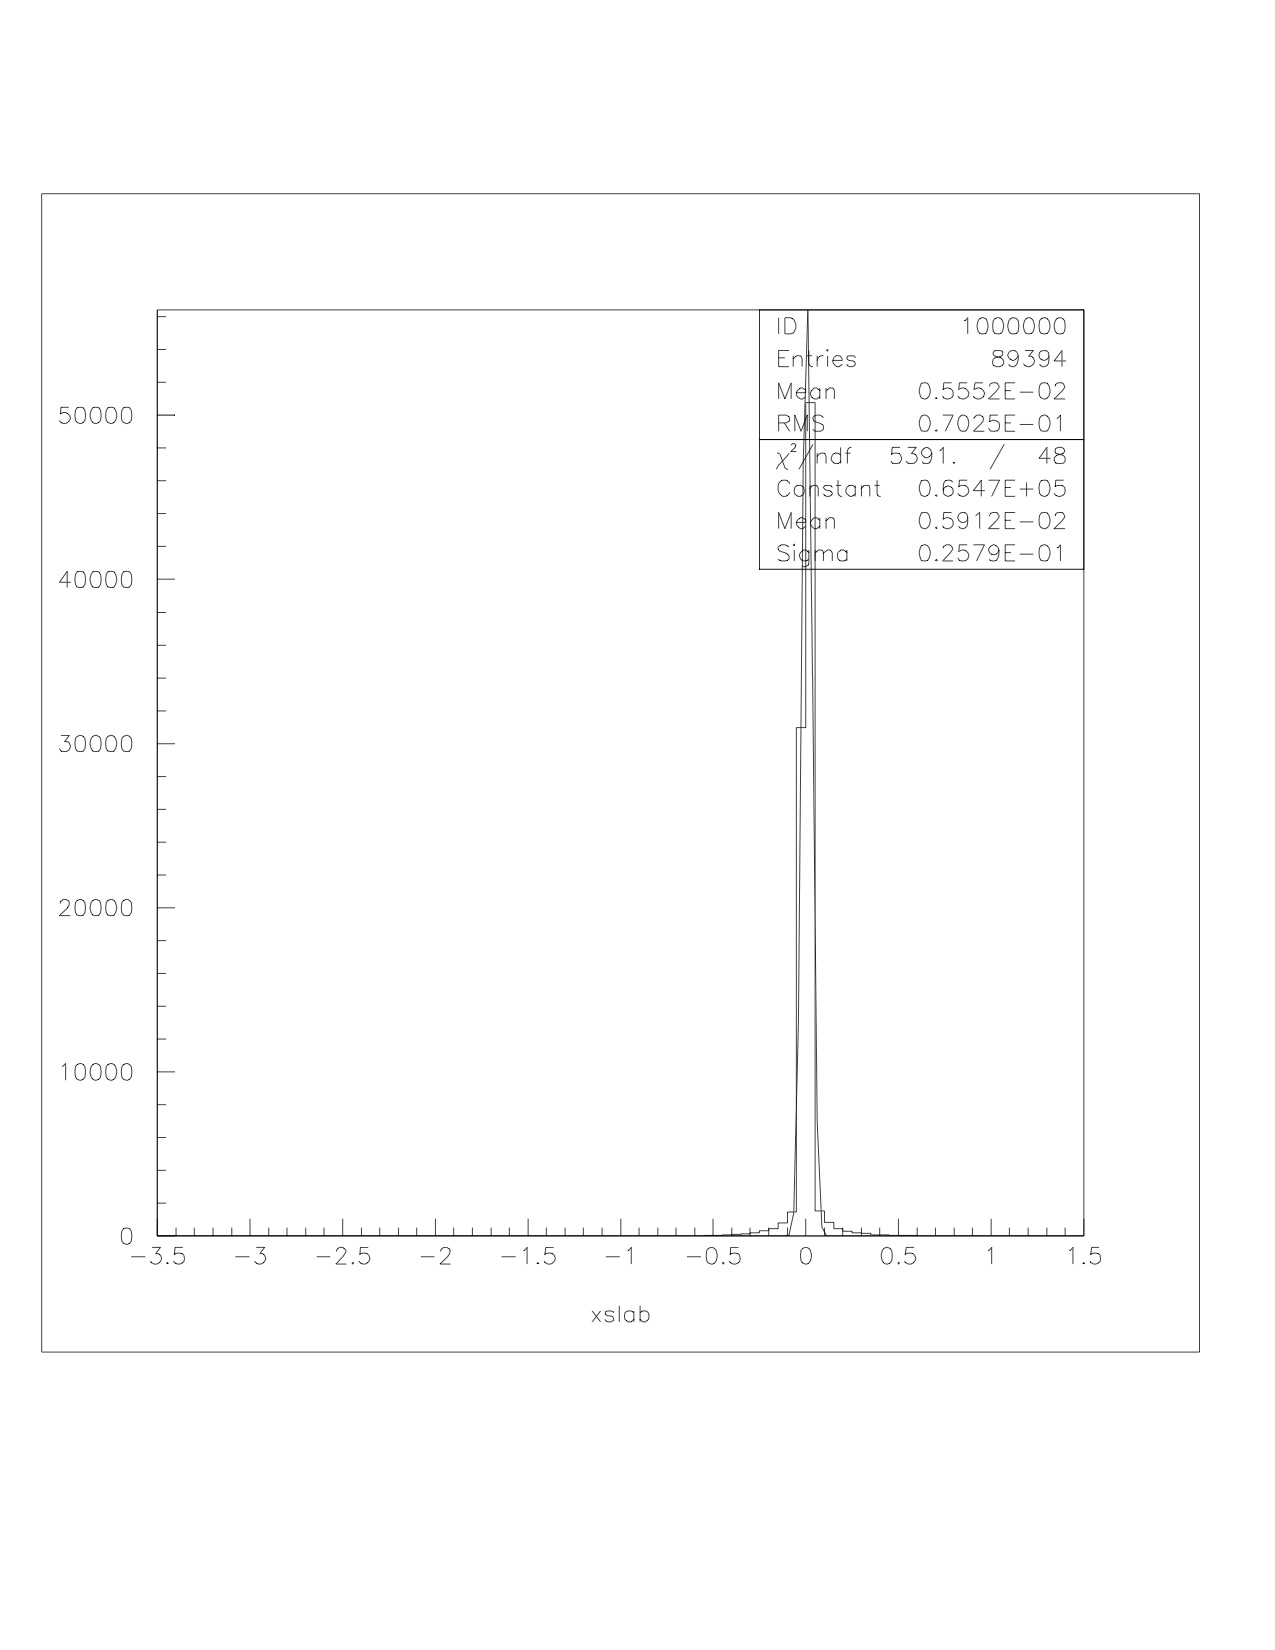
\includegraphics[width=0.45\textwidth]{ex_images/1_100_140_xs.jpg}}
  \caption{PSF plots with detector thickness of 10 mm, no blur.}
  \label{fig:100_xs}
\end{figure}

\begin{figure}[H]
  \centering
  \subfloat[][$\gamma$ energy $=$ 10 KeV] {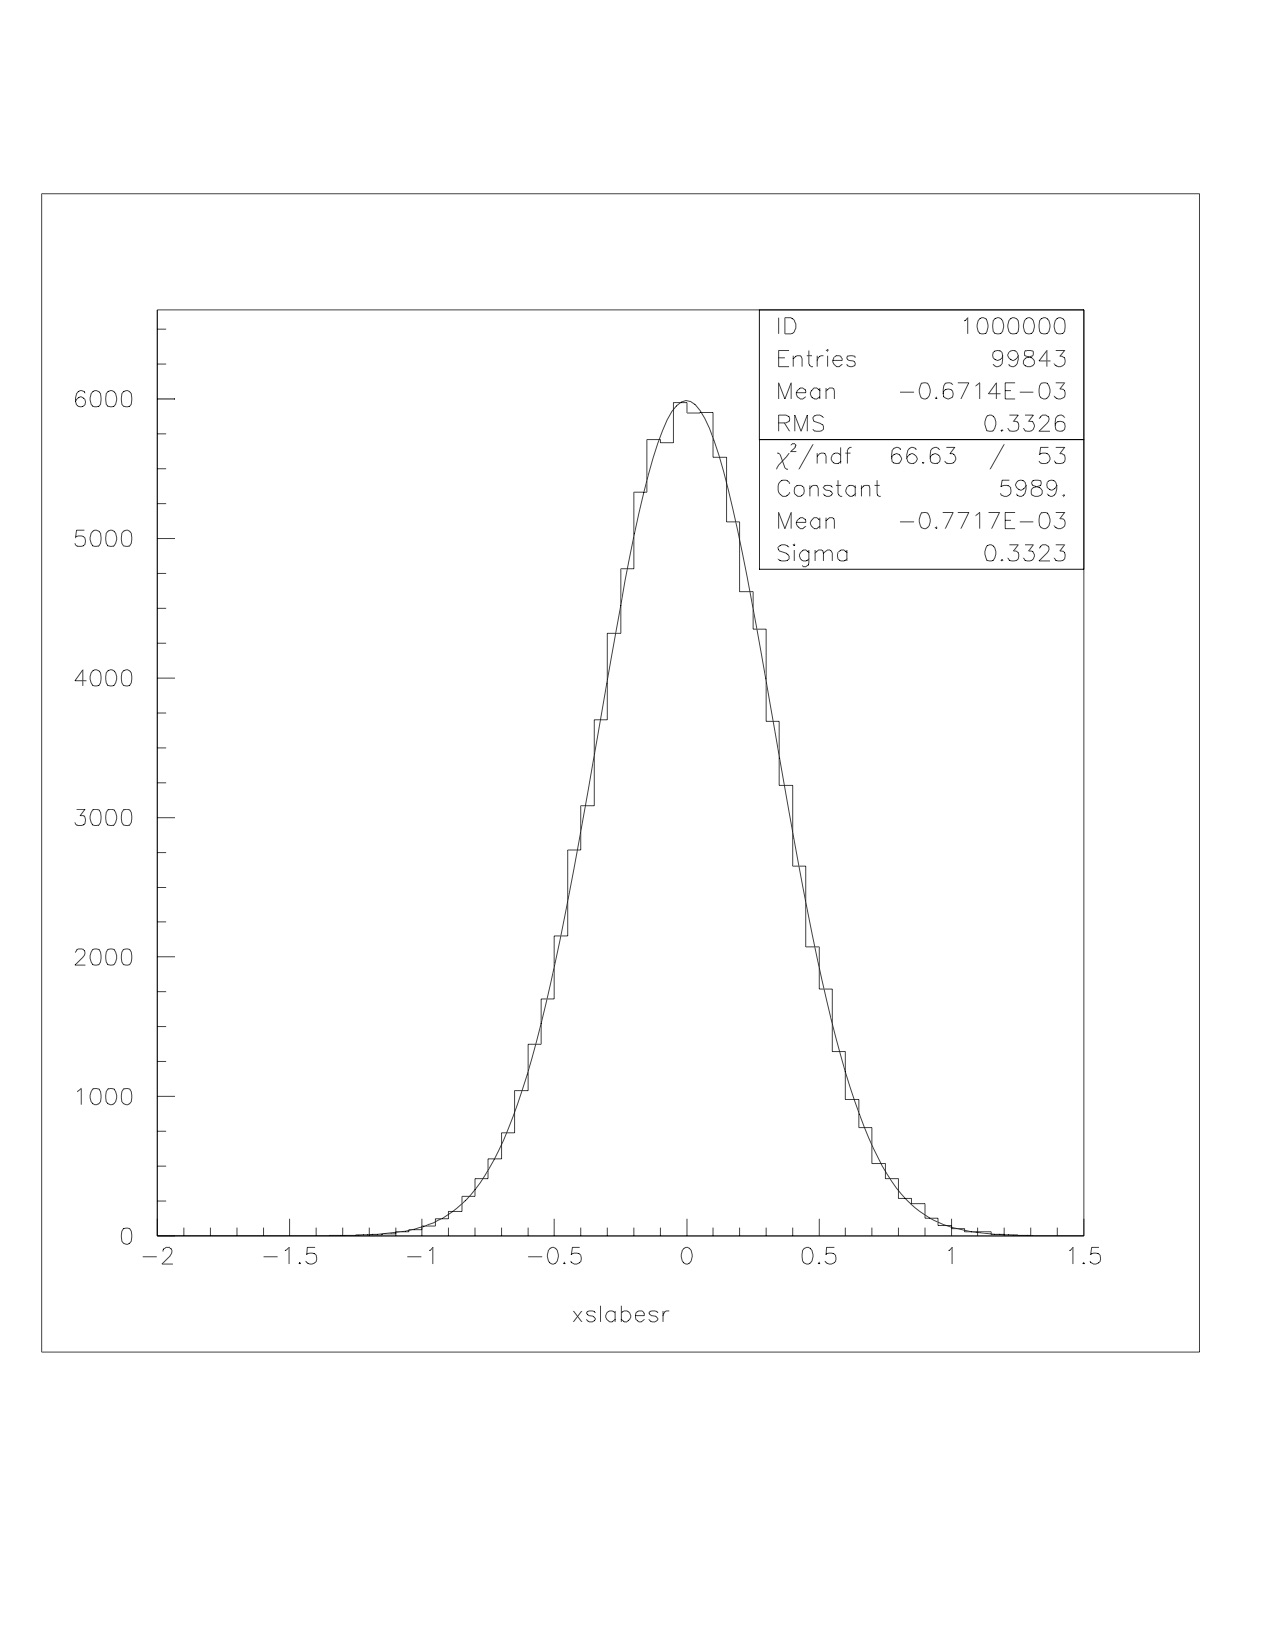
\includegraphics[width=0.45\textwidth]{ex_images/1_100_010_xse.jpg}}
  \subfloat[][$\gamma$ energy $=$ 30 KeV] {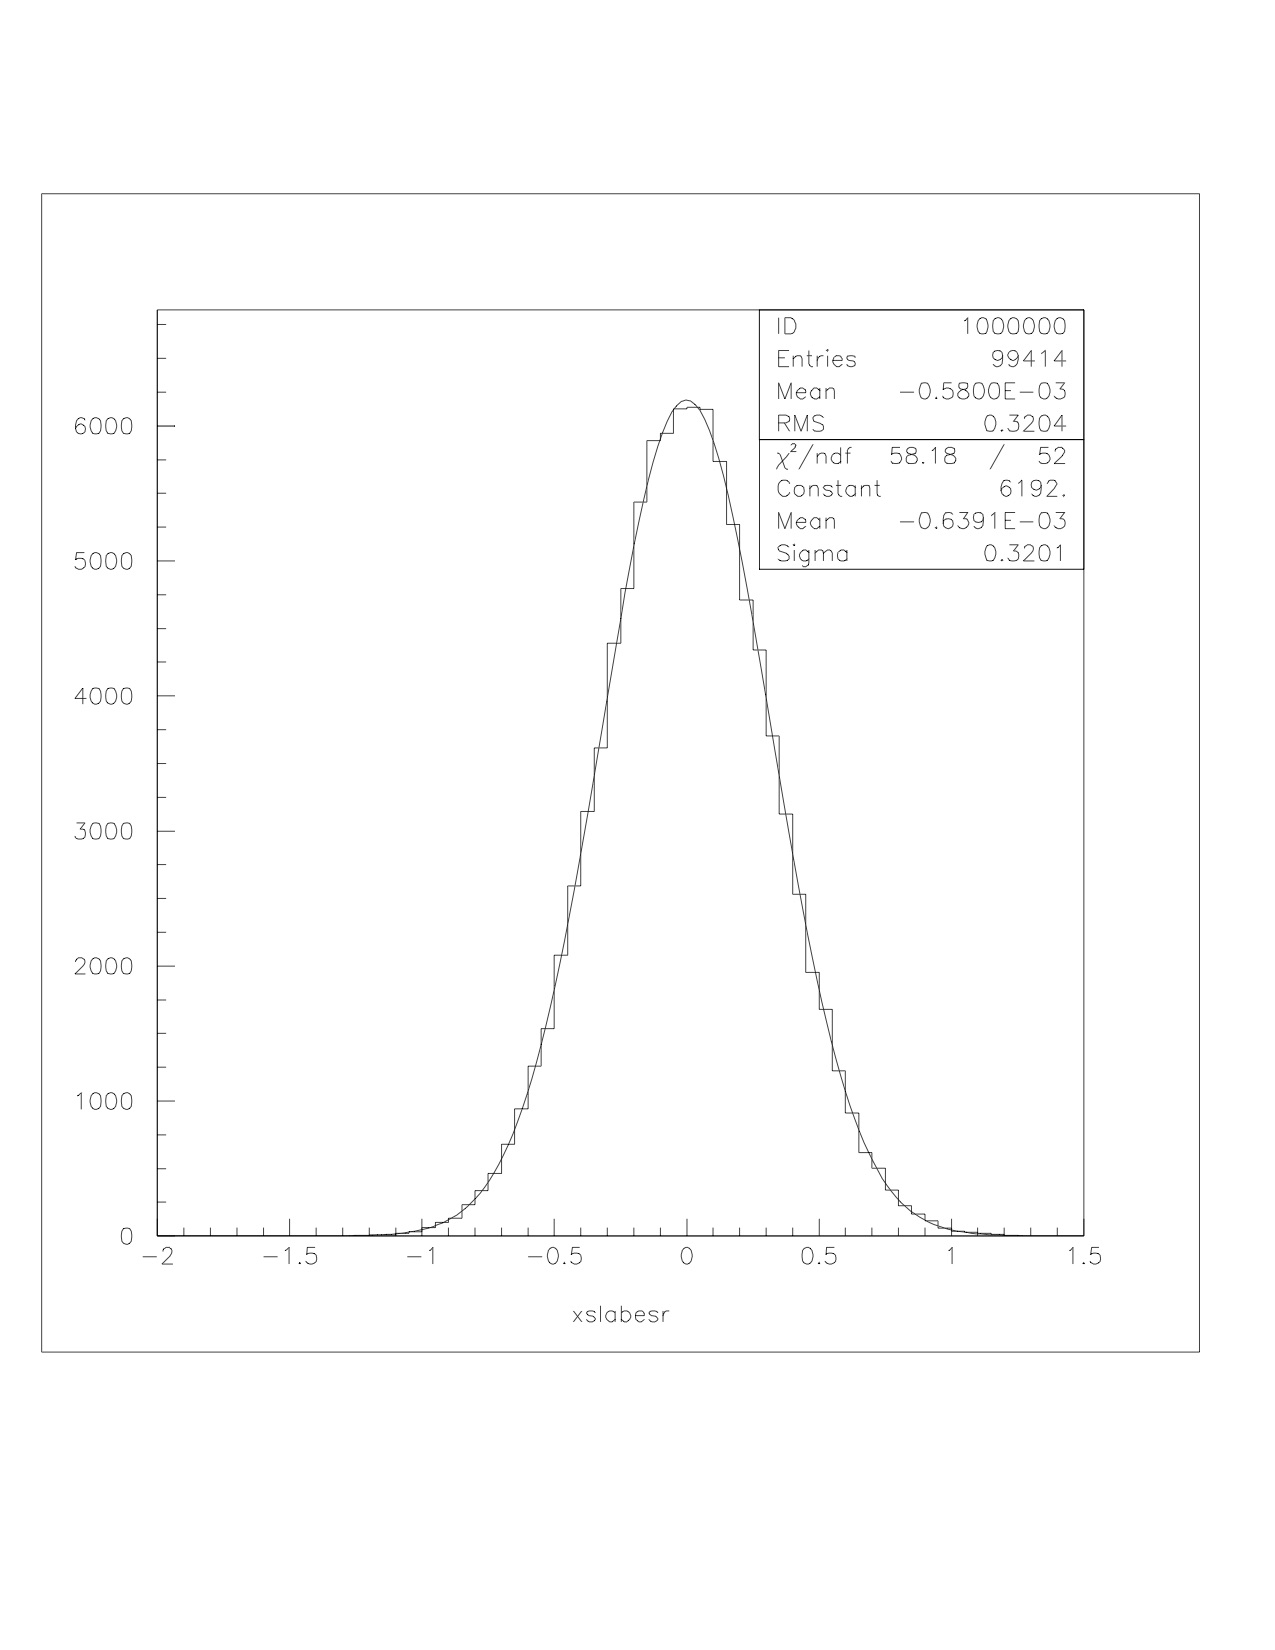
\includegraphics[width=0.45\textwidth]{ex_images/1_100_030_xse.jpg}}\\
  \subfloat[][$\gamma$ energy $=$ 50 KeV] {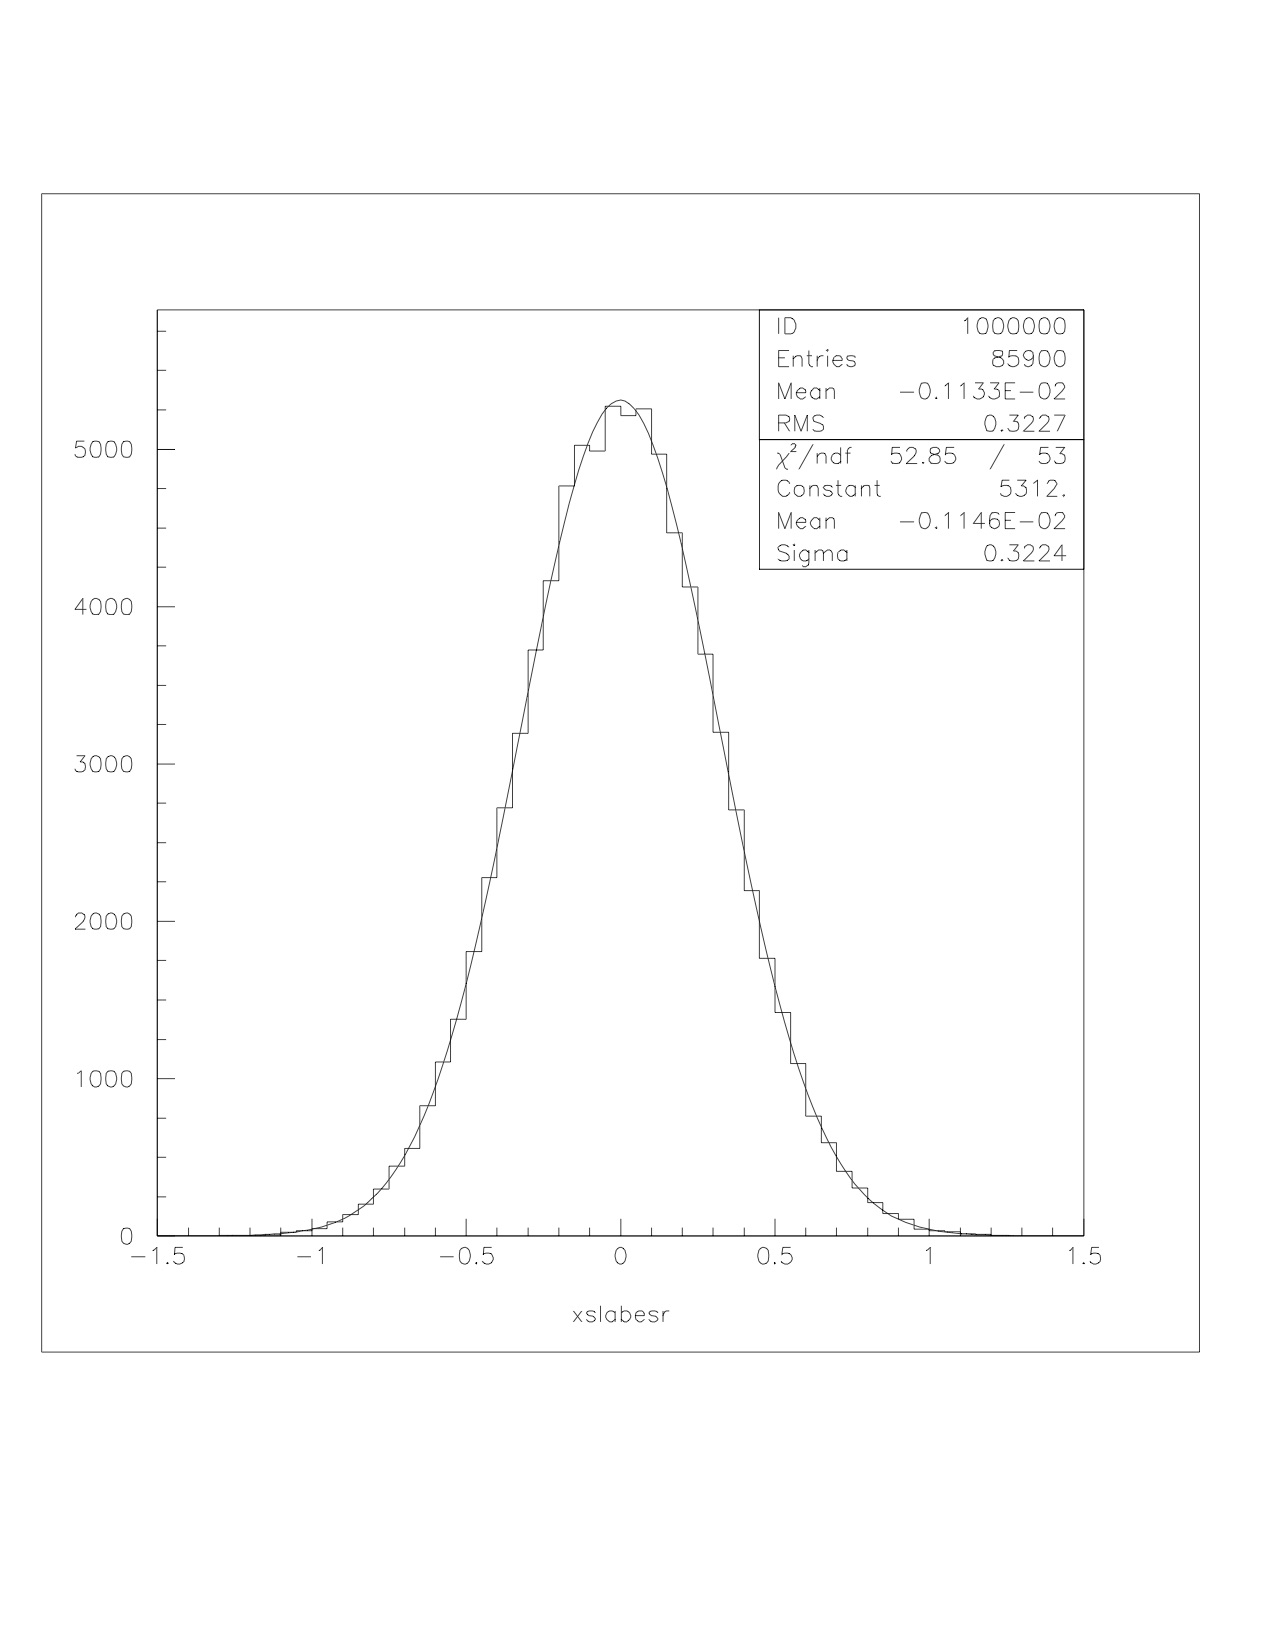
\includegraphics[width=0.45\textwidth]{ex_images/1_100_050_xse.jpg}}
  \subfloat[][$\gamma$ energy $=$ 140 KeV] {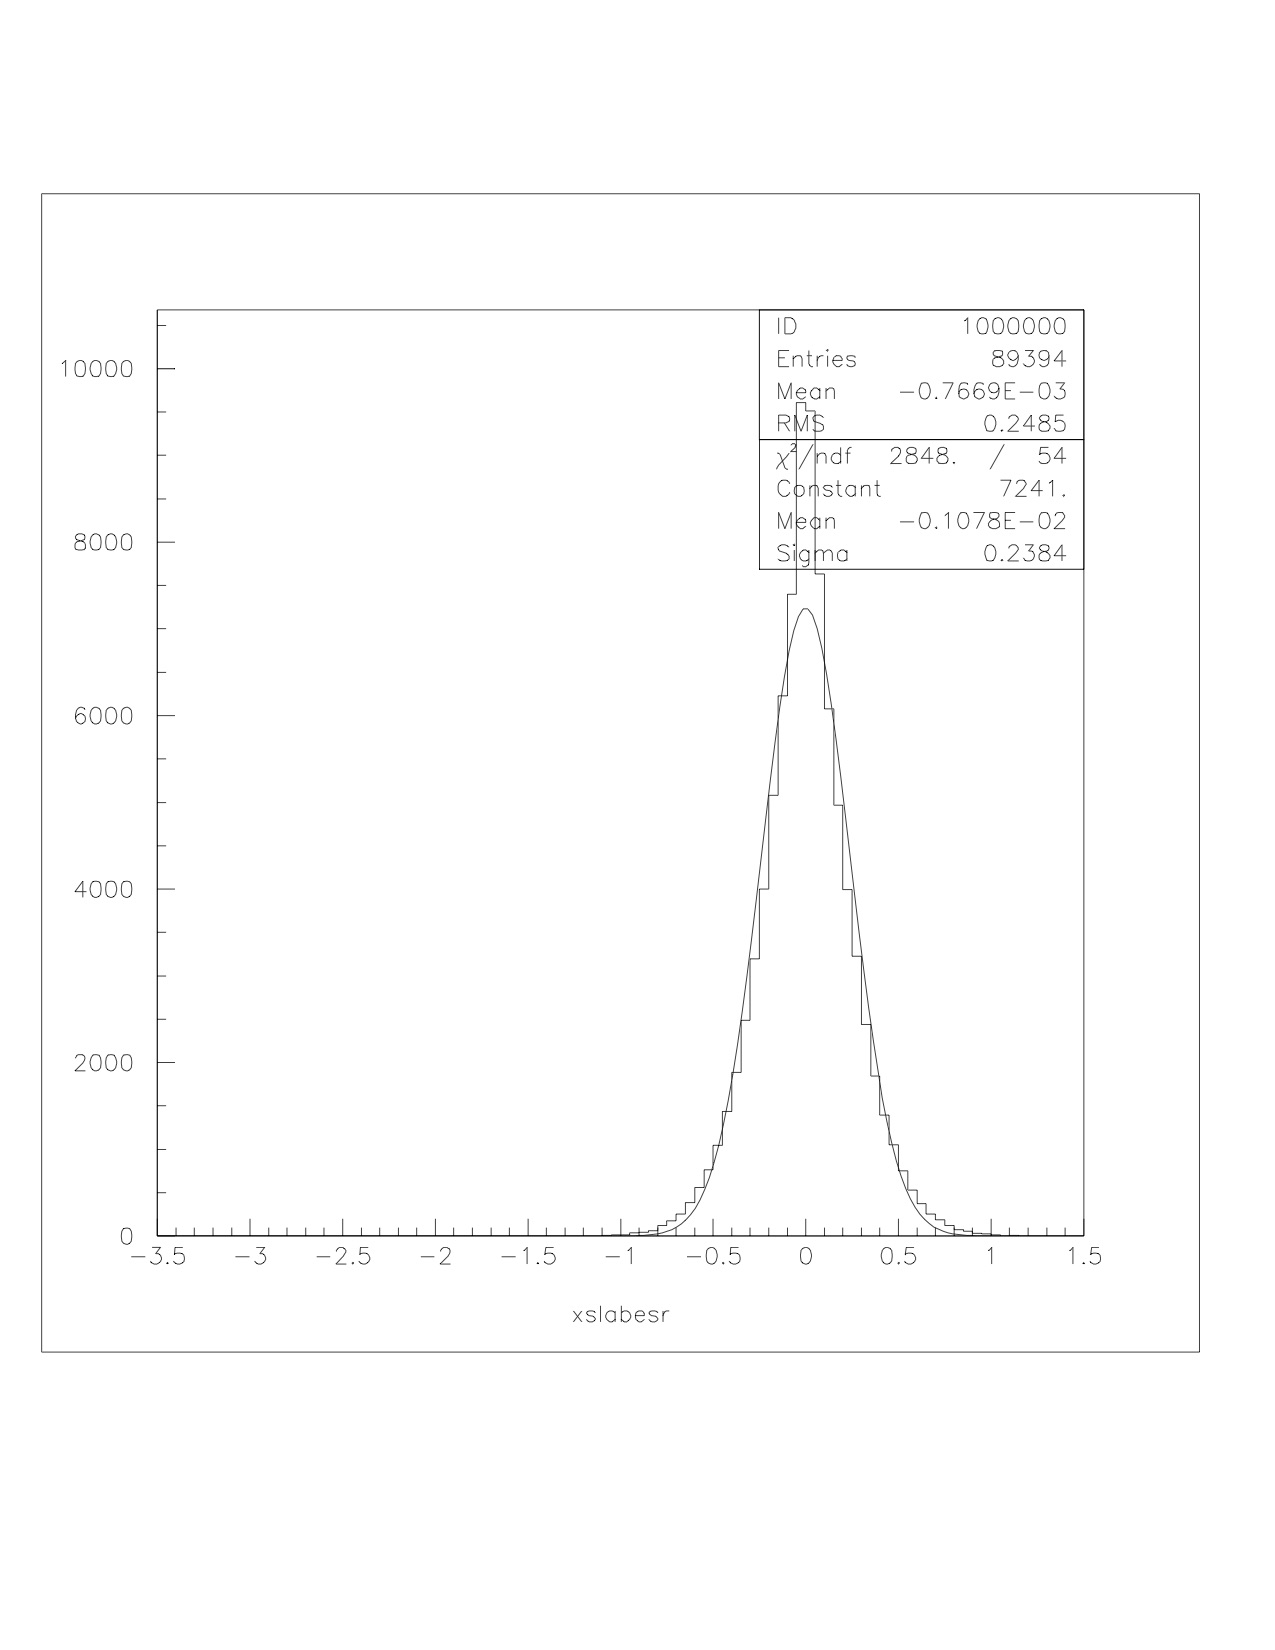
\includegraphics[width=0.45\textwidth]{ex_images/1_100_140_xse.jpg}}
  \caption{PSF plots with detector thickness of 10 mm, with blur.}
  \label{fig:100_xse}
\end{figure}

\section{Plots for the second part}
\label{sec:appendix_2}

\begin{figure}[H]
  \centering
  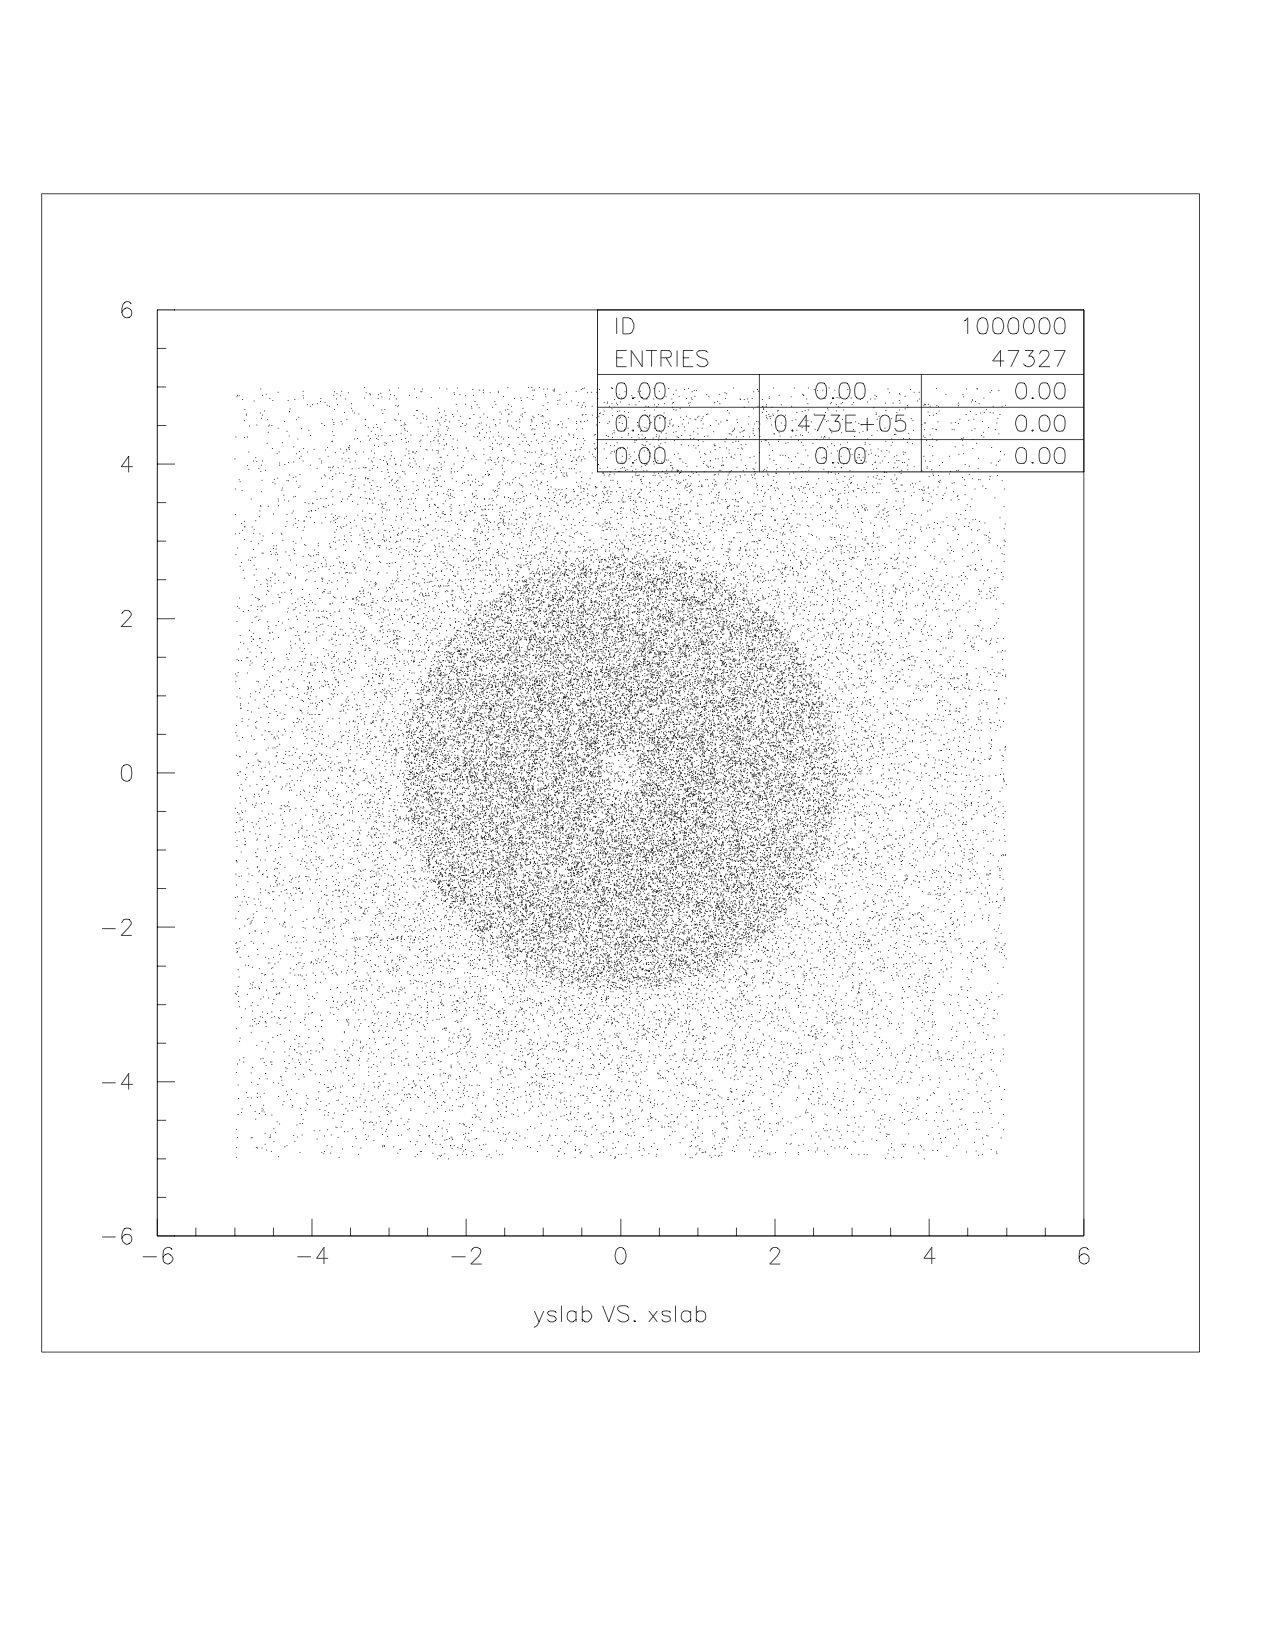
\includegraphics[width=0.9\textwidth]{ex_images/2_2d_10.jpg}
  \caption{moltobello}
  \label{fig:2_2d}
\end{figure}

\begin{figure}[H]
  \centering
  \subfloat[][Box thickness $=$ 4 mm] {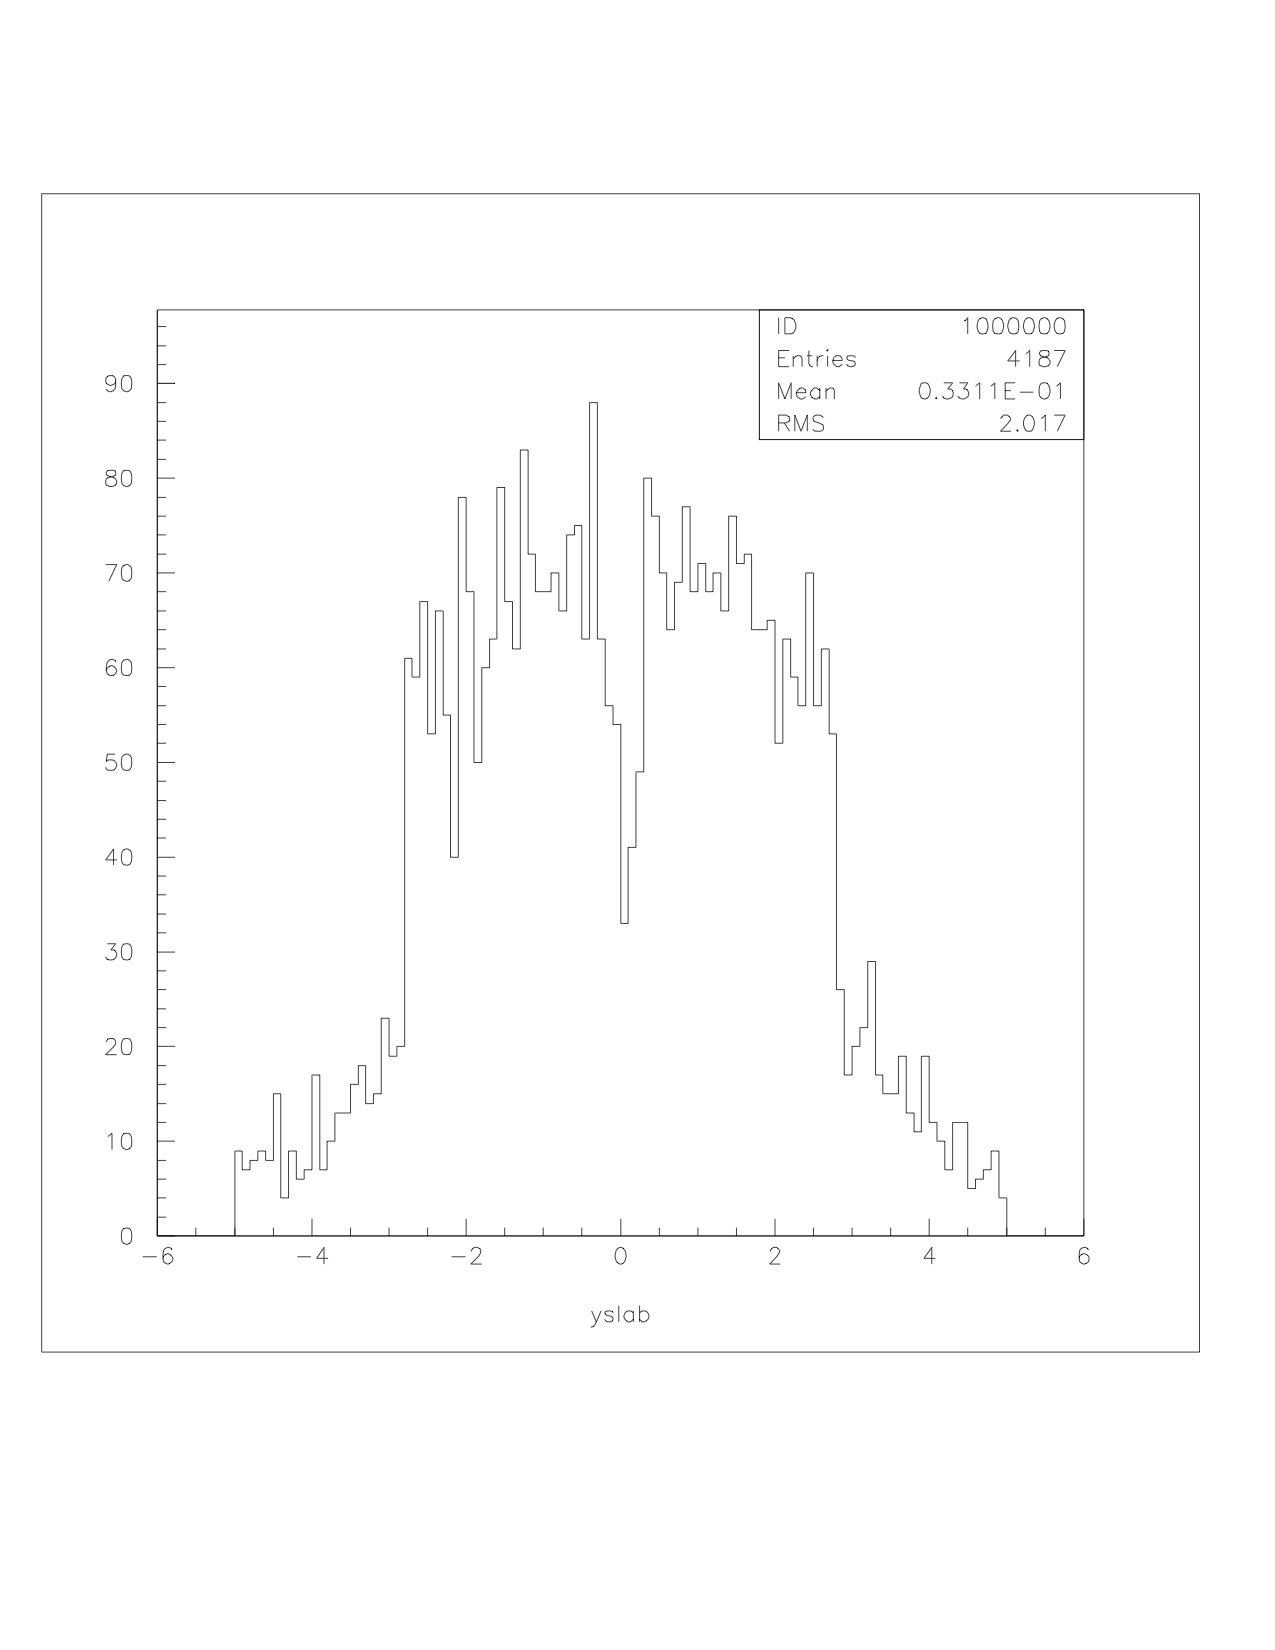
\includegraphics[width=0.45\textwidth]{ex_images/2_cut_04.jpg}}
  \subfloat[][Box thickness $=$ 6 mm] {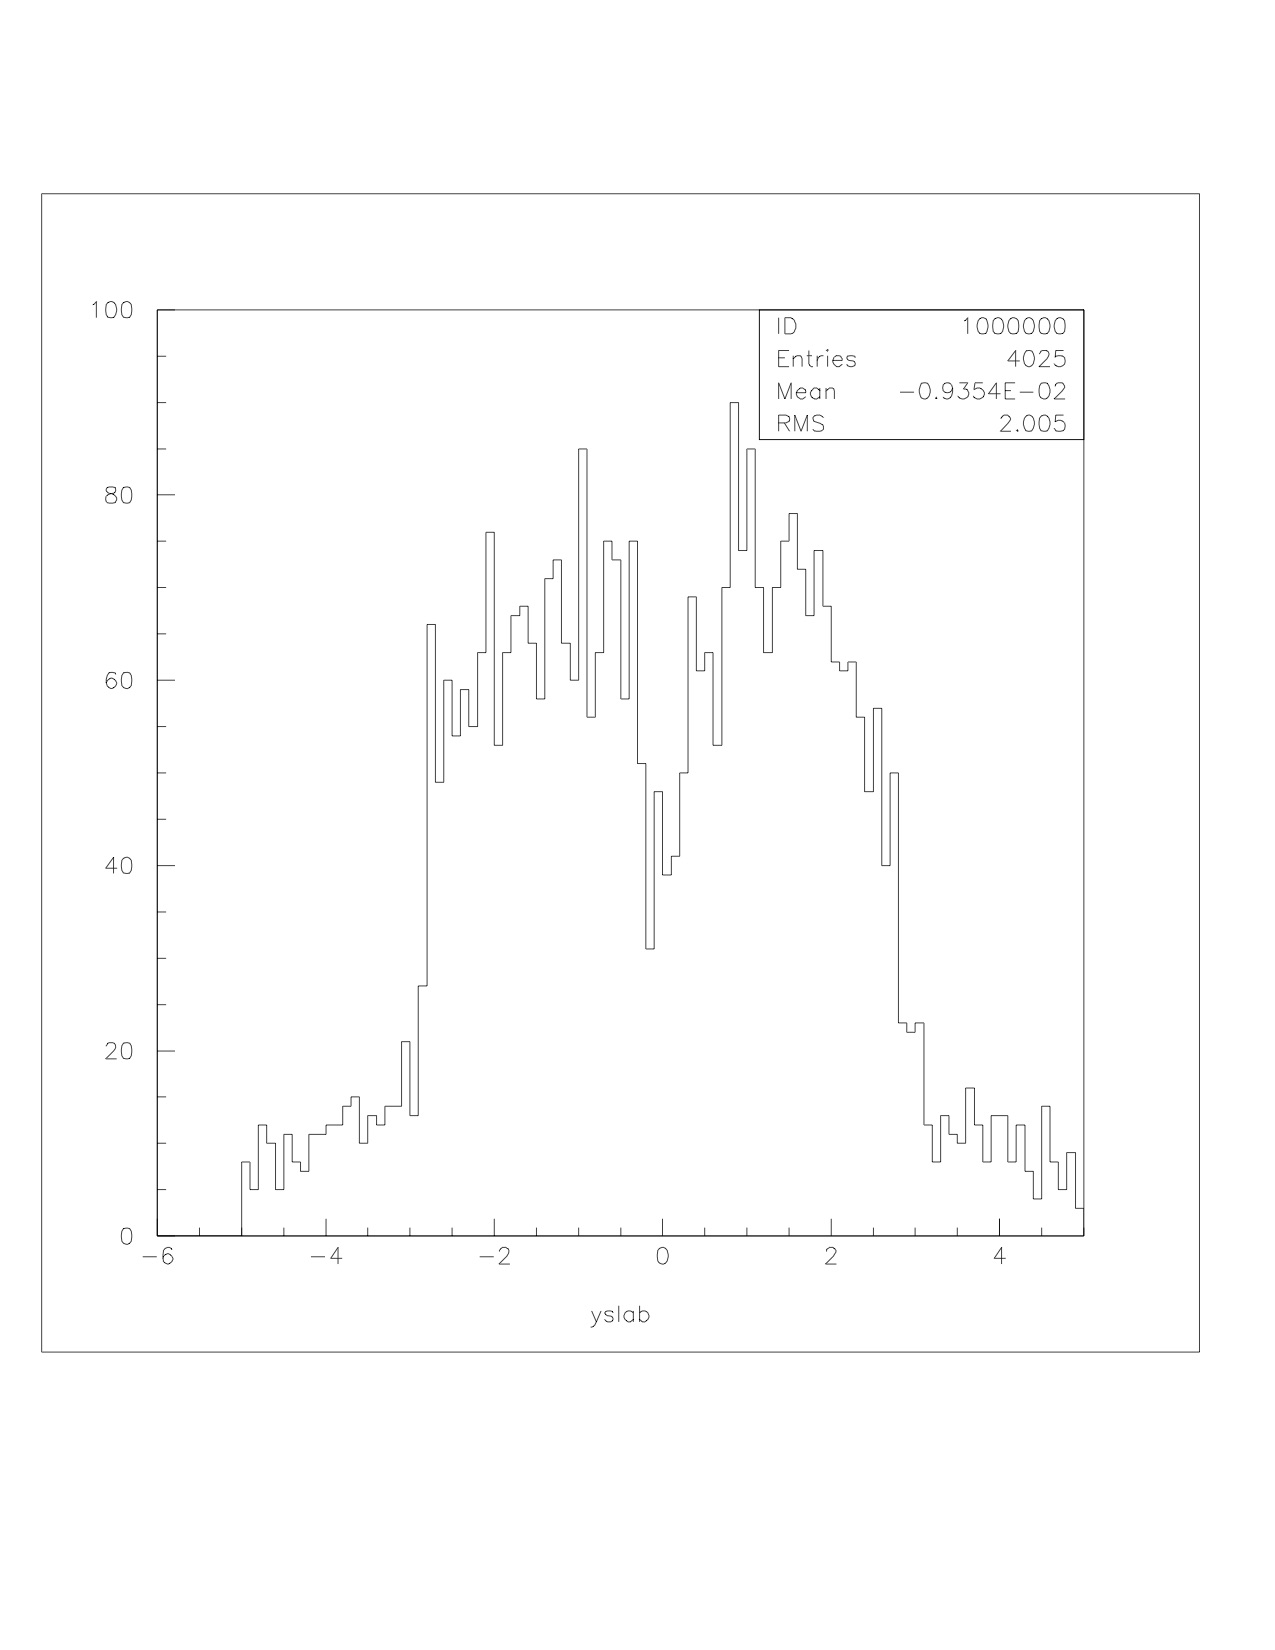
\includegraphics[width=0.45\textwidth]{ex_images/2_cut_06.jpg}}\\
  \subfloat[][Box thickness $=$ 8 mm] {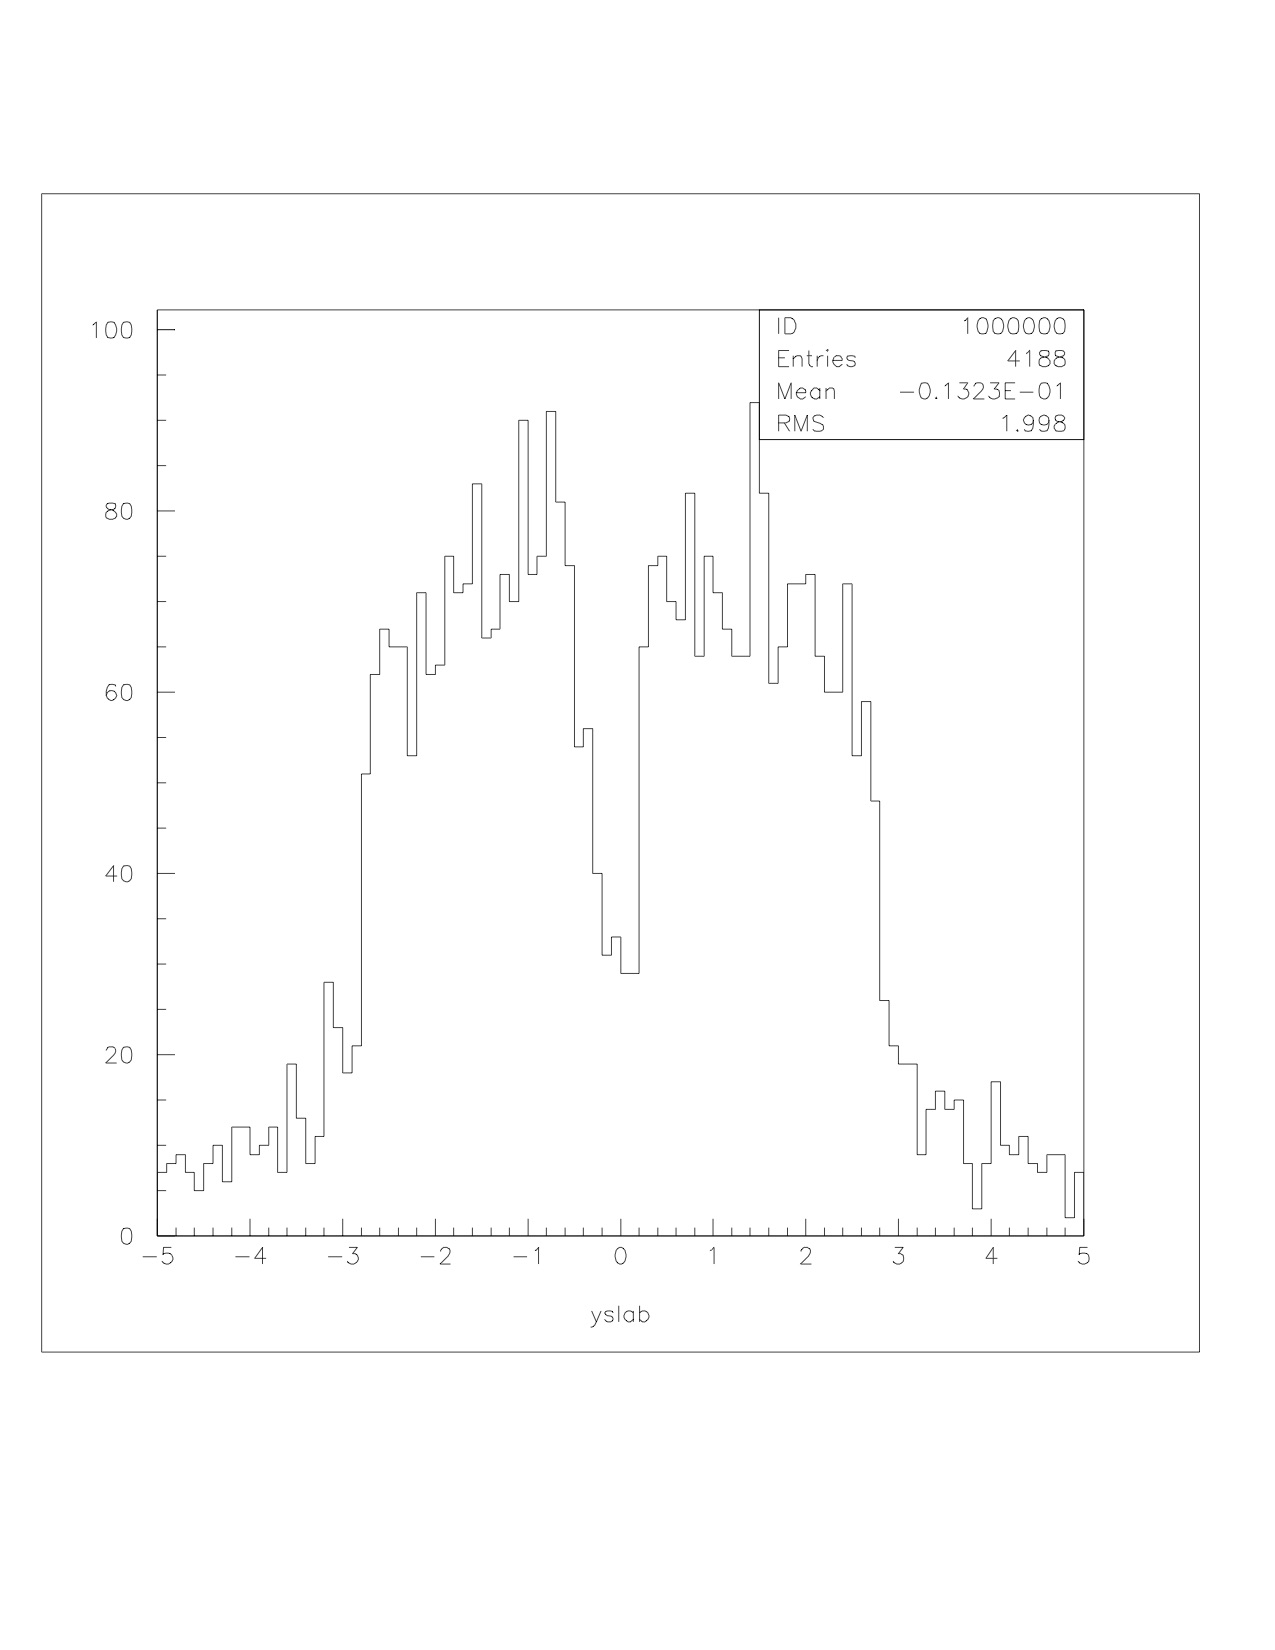
\includegraphics[width=0.45\textwidth]{ex_images/2_cut_08.jpg}}
  \subfloat[][Box thickness $=$ 10 mm] {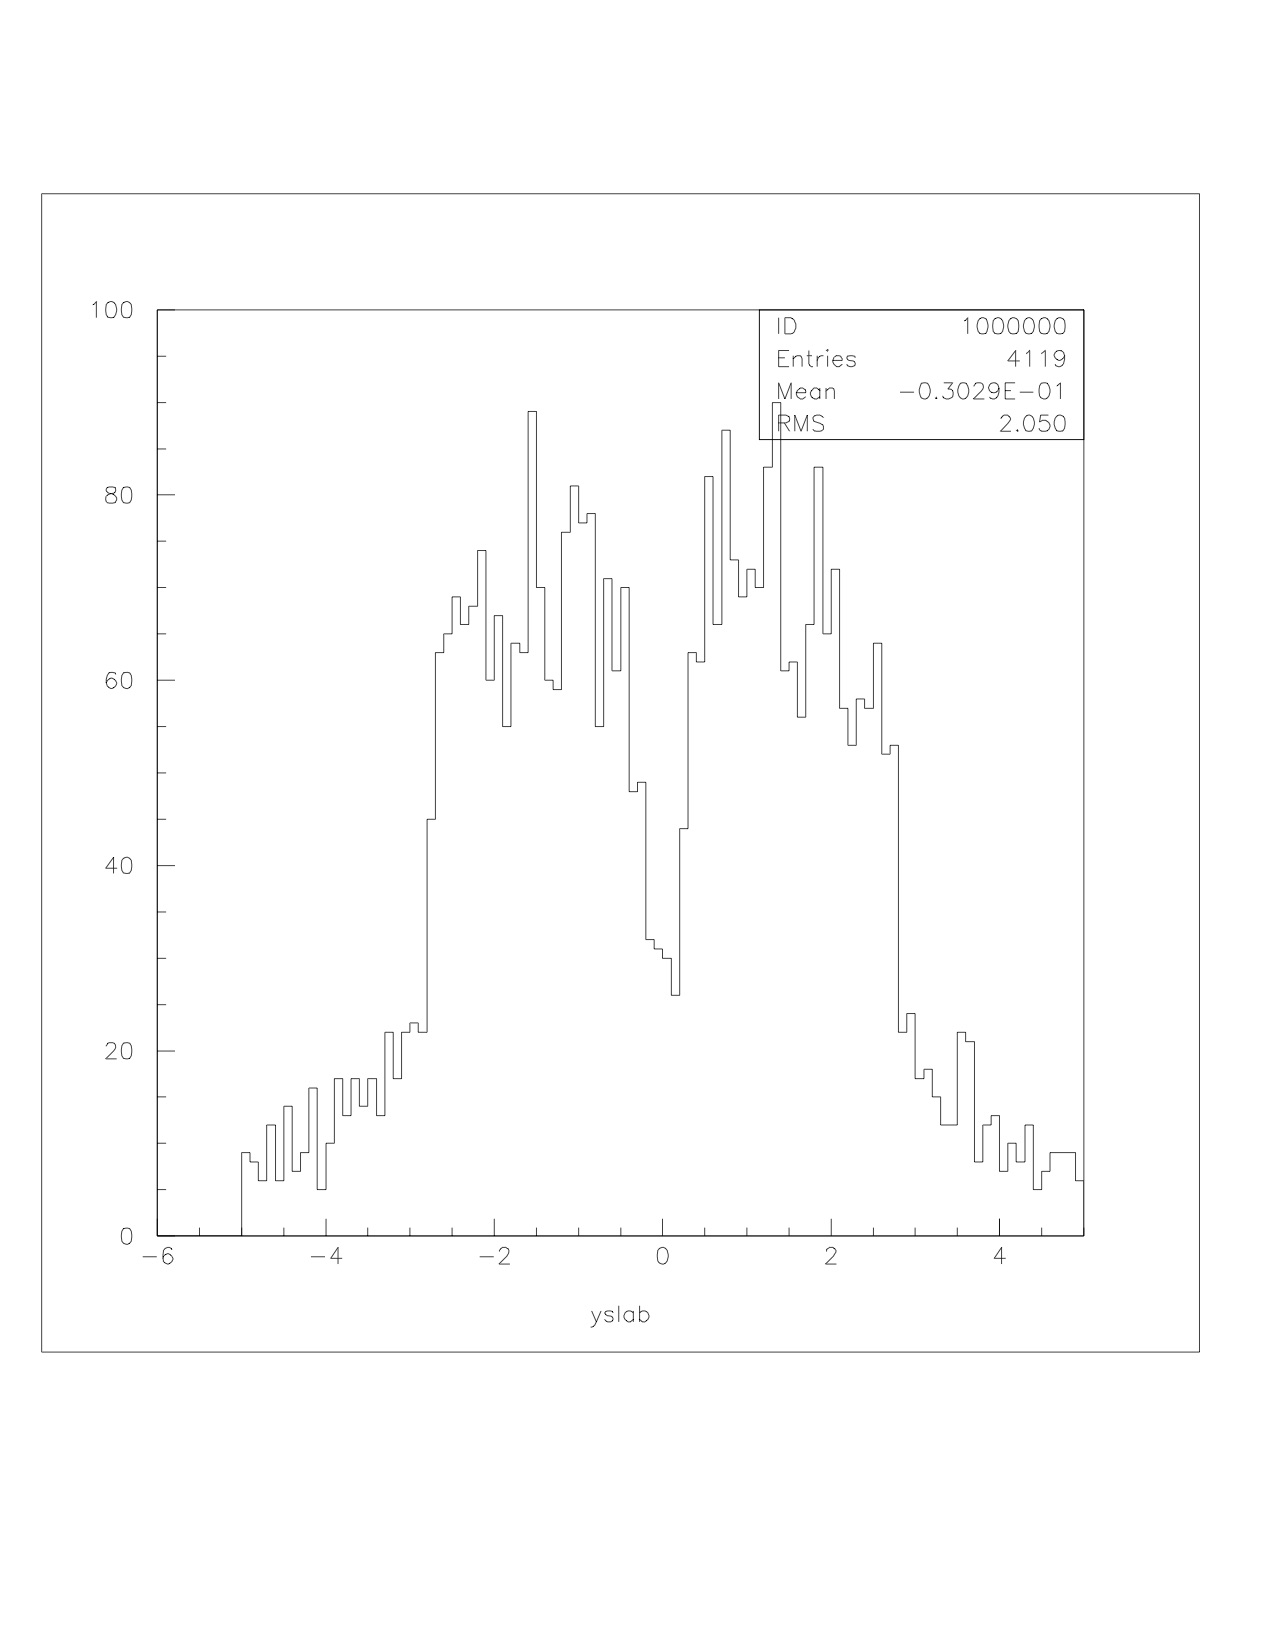
\includegraphics[width=0.45\textwidth]{ex_images/2_cut_contrast_10.jpg}}
  \caption{moltobello anche questp}
  \label{fig:2_all}
\end{figure}

\end{document}








